% -----------------------------------------------------------------------------
% Project: PhD KAPPA
% File: kappa.Rnw (root file)
% Author: Alessio Crippa
% Template: based on the tex code written by Andrea Discacciati
%           url: https://github.com/anddis/phd-thesis
%
% Purpose: Root Rnw file, compile this to typeset the kappa!
% -----------------------------------------------------------------------------



% If you get the following error:
%  Error in ensurePackageSymlink(source, target) :
% run the next line, an then restart your R session
% unlink("packrat/lib-R", recursive = TRUE)


% Class
\documentclass[11pt,a4paper,twoside,openany]{book}\usepackage{knitr}

% Packages
\usepackage[english]{babel}
\usepackage{amsfonts}
\usepackage{amsmath}
\usepackage{mathtools}
\usepackage{threeparttable}
\usepackage{adjustbox}
\usepackage{natbib}
\usepackage{graphicx}
\usepackage{flafter}
\usepackage{fancyhdr}
\usepackage{textcomp}
\usepackage[utf8]{inputenc}
\usepackage{setspace}
\usepackage[pdftex,
            pdfauthor={Alessio Crippa},
            pdftitle={Novel methods for dose--response meta-analysis},
            pdfcreator={LaTeX2e}]{hyperref}
\usepackage[%showframe,
			headheight=13.6pt,
			%headsep=,
			%footskip=,
			bindingoffset=0cm,%print=.5cm, web=0cm
			left=3cm,  %print=2cm, web=3cm
			bottom=3cm, %print=3cm, web=3cm
			top=3cm, %print=3cm, web=3cm,
			right=3cm]{geometry} %print=3.5cm, web=3cm
\usepackage{enumerate, mdwlist}
\usepackage{etoolbox}
\usepackage{tabularx}
\usepackage{float}
\usepackage{rotating}
\usepackage{lscape}
\usepackage{longtable}
\usepackage[font={small}]{caption}
\usepackage{chngcntr}
\usepackage{booktabs}
\counterwithout{footnote}{chapter}



%---begin see http://www.khirevich.com/latex/font/
\usepackage[activate={true,nocompatibility},final,tracking=true,kerning=true,spacing=true,factor=1100, stretch=10,shrink=10]{microtype}
% remove warning
\microtypecontext{spacing = nonfrench}
\usepackage[T1]{fontenc}
% remove warning
\global\expandafter\let\csname ver@amsfonts.sty\endcsname\relax
% remove issue related to interwordspace
\setlength{\emergencystretch}{10pt}
\usepackage[bitstream-charter]{mathdesign}
\usepackage{sectsty}
	\chapterfont{\usefont{T1}{qhv}{b}{n}\selectfont\huge}
\usepackage{titlesec}

% ---------------------------------------------------------
% Project: PhD KAPPA
% File: _titlesec.tex
% Author: Andrea Discacciati
%
% Purpose: Headings format
%			(see titlesec package)
% ---------------------------------------------------------

\titleformat{\section}[hang]{
    \usefont{OT1}{qhv}{bx}{n}\selectfont}
    {} 
    {0em}
    {\hspace{-0.4pt}\Large \thesection\hspace{0.6em}}
\titleformat{\subsection}[hang]{
    \usefont{OT1}{qhv}{bx}{n}\selectfont}
    {} 
    {0em}
    {\hspace{-4pt} \thesubsection\hspace{0.6em}}
\titleformat{\subsubsection}[hang]{
    \usefont{OT1}{qhv}{bx}{n}\selectfont}
    {} 
    {0em}
    {\normalsize}
\usepackage{tocloft}

% ---------------------------------------------------------
% Project: PhD KAPPA
% File: _tocloft.tex
% Author: Andrea Discacciati
%
% Purpose: Table of Contents, 
%			List of Figures, List of Tables format
%			(see tocloft package)
% ---------------------------------------------------------

\renewcommand{\cfttoctitlefont} % ToC title
             {\usefont{T1}{qhv}{b}{n}\selectfont\huge}
\renewcommand{\cftchapfont} % chapter titles
             {\usefont{T1}{qhv}{b}{n}\selectfont}
\renewcommand{\cftsecfont} % section titles
             {\usefont{T1}{bch}{m}{n}\selectfont}
\renewcommand{\cftsubsecfont} % subsection titles
             {\usefont{T1}{bch}{m}{n}\selectfont} 
\renewcommand{\cftchappagefont} % chapter page numbers
             {\usefont{T1}{bch}{b}{n}\selectfont}
\renewcommand{\cftsecpagefont} % section page numbers
             {\cftsecfont} 
\renewcommand{\cftsubsecpagefont} % subsection page numbers
             {\cftsubsecfont}
             
\renewcommand{\cftloftitlefont} % LoF title
             {\usefont{T1}{qhv}{b}{n}\selectfont\huge}
\renewcommand{\cftfigfont} % Figures titles
             {\usefont{T1}{bch}{m}{n}\selectfont}
             
\renewcommand{\cftlottitlefont} % LoT title
             {\usefont{T1}{qhv}{b}{n}\selectfont\huge}
\renewcommand{\cfttabfont} % Tables titles
             {\usefont{T1}{bch}{m}{n}\selectfont}
%---end see http://www.khirevich.com/latex/font/

% Header / footer

% ---------------------------------------------------------
% Project: PhD KAPPA
% File: _fancyhdr.tex
% Author: Alessio Crippa
% based on the template written by Andrea Discacciati
%
% Purpose: Header and footer settings
%			(see fancyhdr package)
% ---------------------------------------------------------

\pagestyle{fancy}
\renewcommand{\chaptermark}[1]{%
 \markboth{{\thechapter.\ #1}}{}}

\fancypagestyle{plain}{%
  \fancyhf{}%
  \renewcommand{\headrulewidth}{0pt}%
  \fancyhf[lef,rof]{}%
  %\fancyhead[LE,RO]{\thepage}
}

\fancypagestyle{frontmatter}{%
  \renewcommand{\headrulewidth}{0pt} 
  \renewcommand{\footrulewidth}{0pt}
  \fancyhf{}% Clear header/footer
  \fancyhead[LE,RO]{}
}

\fancypagestyle{nothing}{%
  \renewcommand{\headrulewidth}{0pt} 
  \renewcommand{\footrulewidth}{0pt}
  \fancyhf{}% Clear header/footer
  \fancyhead[LE,RO]{}%
}

\fancypagestyle{mainmatter}{%
  \renewcommand{\headrulewidth}{.4pt}
  \renewcommand{\footrulewidth}{0pt}
  \fancyhf{}% Clear header/footer
  \fancyhead[LE,RO]{\thepage}
  \fancyhead[RE,LO]{\nouppercase \leftmark}
}

	
% See 'writing a thesis with latex' p25 
% Writes nothing on empty pages
\makeatletter
\def\cleardoublepage{\clearpage\if@twoside
\ifodd\c@page
\else\hbox{}\thispagestyle{empty}\newpage
\if@twocolumn\hbox{}\newpage\fi\fi\fi}
\makeatother

% Substitutions (%examples)
%\newcommand{\rveplot}{decorrelated-residuals--versus--exposure plot}
%\newcommand{\kgmsq}{kg$\times$m\textsuperscript{$-2$}}
\newcommand{\pkg}[1]{{\fontseries{b}\selectfont #1}}

\defcitealias{crippa2016dosresmeta}{Paper~I}	
\defcitealias{discacciati2015goodness}{Paper~II}	
\defcitealias{crippa2016new}{Paper~III}	
\defcitealias{crippa2018pointwise}{Paper~IV}	
\defcitealias{crippa2018one}{Paper~V}	

%\doublespacing 
\onehalfspacing

\allowdisplaybreaks

\renewcommand{\sfdefault}{qhv}
\newcommand*{\LargerCdot}{\raisebox{-0.25ex}{\scalebox{1.2}{$\cdot$}}}

\DeclareMathOperator{\R}{\textsf{R}}
\DeclareMathOperator{\Var}{Var}
\DeclareMathOperator{\SE}{SE}
\DeclareMathOperator{\Cov}{Cov} 
\DeclareMathOperator{\diag}{diag} 
\DeclareMathOperator{\N}{N} 
\DeclareMathOperator{\E}{E}
\DeclareMathOperator{\logit}{logit} 
\DeclareMathOperator{\df}{df} 
\hyphenation{logRRs}
\hyphenation{logRR}

\addto\captionsenglish{%
  \renewcommand{\bibname}{References}%
}

%\includeonly{abstract, results, introduction, background, aims, discussion, conclusions }

%--- Kappa starts here! ---%
\IfFileExists{upquote.sty}{\usepackage{upquote}}{}
\begin{document}

% Front matter
\frontmatter
\pagestyle{nothing}

% ---------------------------------------------------------
% Project: PhD KAPPA
% File: titlepage.tex
% Author: Alessio Crippa
% based on the template written by Andrea Discacciati
%
% Purpose: Custom title page + ISBN/copyright page
% ---------------------------------------------------------

\begin{titlepage}
\newgeometry{margin=4cm}
\begin{center}
\large
From the Department of Public Health Sciences \\
Karolinska Institutet, Stockholm, Sweden        
\vfill
\Large
\textbf{\textsf{NOVEL METHODS FOR DOSE-RESPONSE META-ANALYSIS}}
\vfill
\Large
Alessio Crippa
\vfill

\includegraphics[width=0.8\textwidth]{figures/ki-logo_pos}
\vfill
\large
Stockholm 2018        
\end{center}
\restoregeometry
\end{titlepage}

\newpage
\null
\vfill
\noindent All published papers reproduced with permission \\
Published by Karolinska Institutet \\
\bigskip
Printed by E-Print AB 2018 \\
Edited in R using knitr. \\
Codes to compile this thesis are available at \url{https://github.com/alecri/kappa} \\
\textcopyright Alessio Crippa, 2018 \\
ISBN <include number>
\newpage

% ---------------------------------------------------------
% Project: PhD KAPPA
% File: spikblad.tex
% Author: Alessio Crippa
% based on the template written by Andrea Discacciati
%
% Purpose: Spikblad
% ---------------------------------------------------------
\null
\vspace{1.5cm}
\noindent{\Large \textsf{NOVEL METHODS FOR DOSE-RESPONSE META-ANALYSIS} \vspace{1cm}}\\
\noindent{\Large \textsf{THESIS FOR DOCTORAL DEGREE (Ph.D.)} \vspace{.5cm}}\\
By \vspace{.5cm} \\
{\Large \textbf{\textsf{Alessio Crippa}} \vspace{2cm}}\\
\begin{minipage}[t]{6.2cm}
\singlespacing
{\small
\textit{Principal supervisor:}\\
Associate Professor Nicola Orsini \\
Karolinska Institutet \\
\bigskip
Department of Public Health Sciences \\
\textit{Co-supervisor:}\\
Professor Alicja Wolk \\
Karolinska Institutet \\
\medskip
Institute of Environmental Medicine \\
Professor Matteo Bottai \\
Karolinska Institutet \\
\medskip
Institute of Environmental Medicine \\
Professor Donna Spiegelman \\
Harvard T.H. Chan School of Public Health \\
Department of Epidemiology
}
\end{minipage}
\hspace{1.5cm}
\begin{minipage}[t]{8.1cm}
\singlespacing
{\small
\textit{Opponent:}\\
Professor Christopher H. Schmid \\
Brown University \\
Center for Evidence Based Medicine\bigskip \\
\textit{Examination board:}\\
Associate Professor Nele Brusselaers \\
Karolinska Institutet \\
Department of Microbiology, Tumor and Cell Biology \medskip \\
Associate Professor Antonio Gasparrini \\
London School of Hygiene and Tropical Medicine \\
Department of Social $\&$ Environmental Health Research\medskip \\
Professor Paul Lambert \\
University of Leicester \\
Department of Health Sciences
}
\end{minipage}
\cleardoublepage

% ---------------------------------------------------------
% Project: PhD KAPPA
% File: dedication.tex
% Author: Alessio Crippa
% based on the template written by Andrea Discacciati
%
% Purpose: Dedication
% ---------------------------------------------------------

\begin{flushright}
%http://pubmedcentralcanada.ca/pmcc/articles/PMC2550765/pdf/bmj00610-0065.pdf
\null\vspace{\stretch{1}}
\textit{``The function of the expert reviewer is not to be more right than other people, \\
but to be wrong for more sophisticated reasons.''} \\
---Iain Chalmers and Douglas G. Altman \\ 
\textit{Systematic Reviews}, 1995
\vspace{\stretch{2}}\null
\end{flushright}


\iffalse
\begin{flushright}
\null\vspace{\stretch{1}}
\textit{``If I have seen further, it is by standing on the shoulders of giants.''} \\
---Isaac Newton
\vspace{\stretch{2}}\null
\end{flushright}
\fi
\cleardoublepage 
\pagestyle{frontmatter}

% ---------------------------------------------------------
% Project: PhD KAPPA
% File: abstract.tex
% Author: Andrea Discacciati
%
% Purpose: Abstract frontmatter
% ---------------------------------------------------------


\noindent {\Large \textsf{\textbf{{Abstract}}}
\bigskip
%\chapter*{Abstract}
\small
\par Dose--response meta-analysis is a statistical procedure for combining and contrasting the evidence on the association between a continuous exposure and the risk of a health outcome. Different papers refined selected aspects of the methodology, such as implementation of flexible strategies and extensions to multivariate meta-analysis. However, there were still several relevant questions that needed to be addressed. This thesis aims to address these issues by developing and implementing new strategies and ad-hoc measures (\citetalias{crippa2016dosresmeta}), including tools for evaluating the goodness-of-fit (\citetalias{discacciati2015goodness}), a new measure for quantifying the impact of heterogeneity (\citetalias{crippa2016new}), a strategy to deal with differences in the exposure range across studies (\citetalias{crippa2018pointwise}), and a one-stage approach to estimate complex models without excluding relevant studies (\citetalias{crippa2018one}).

In \citetalias{crippa2016dosresmeta}, we described the implementation of the main aspects of the methodology in the \pkg{dosresmeta} $\R$ package available on CRAN. Dedicated functions were written to facilitate specific tasks such as definition of the design matrix and prediction of the pooled results. We illustrated how to estimate both linear and non-linear curves, conduct test of hypotheses, and present the results in a tabular and graphical format reanalyzing published aggregated dose--response data.

In \citetalias{discacciati2015goodness}, we discussed how to evaluate the goodness-of-fit. The proposed solutions consist of descriptive measures to summarize the agreement between fitted and observed data (the deviance and the coefficient of determination), and graphical tools to visualize the fit of the model (decorrelated residuals-versus-exposure plot). A reanalysis of two published meta-analyses exemplified how these tools can improve the practice of quantitative synthesis of aggregated dose--response data. 

In \citetalias{crippa2016new}, we proposed and characterized a new measure, $\hat R_b$, to quantify the proportion of the variance of the pooled estimate attributable to the between-study heterogeneity. Contrary to the available measures of heterogeneity, $\hat R_b$ does not make any assumption about the distribution of the within-study error variances, nor does it require specification of a typical value for these quantities. The performance of the proposed measure was evaluated in an extensive simulation study. We demonstrated how to present and interpret the $\hat R_b$ re-analyzing three published meta-analyses.

In \citetalias{crippa2018pointwise}, we extended a point-wise approach to dose--response meta-analysis of aggregated data. The strategy consists of combining predicted relative risks for a fine grid of exposure values based on potentially different dose--response models. A point-wise approach can improve the flexibility in modeling the study-specific curves and may limit the impact of extrapolation by predicting the study-specific relative risks based on the observe exposure range. We illustrated the methodology using both individual and aggregated participant data.

In \citetalias{crippa2018one}, we formalized a one-stage approach for dose--response meta-analysis in terms of a linear mixed model. We explained the main aspects of the methodology and how to address the same questions frequently answered in a two-stage analysis. Using both hypothetical and real data, we showed how the one-stage approach can facilitate the assessment of heterogeneity over the exposure range, model comparison, and prediction of individual dose--response associations. The main advantage is that flexible curves can be estimated regardless of the number of data-points in the individual analyses.

In conclusion, the methods presented in this thesis enrich the set of tools available for applying dose--response meta-analyses and for addressing specific questions including goodness-of-fit evaluation (\citetalias{discacciati2015goodness}) and quantification of heterogeneity (\citetalias{crippa2016new}). In addition, we presented alternative models for pooling results in case of heterogeneous exposure range (\citetalias{crippa2018pointwise}) and for estimating complex models without excluding relevant studies (\citetalias{crippa2018one}). The proposed methods have been illustrated using real data and implemented in the \pkg{dosresmeta} and \pkg{hetmeta} $\R$ packages available on CRAN (\citetalias{crippa2016dosresmeta}). The codes for reproducing the results of the presented papers, as well as the entire thesis, are available as public repositories on GitHub \url{https://github.com/alecri}.


\normalsize
\cleardoublepage

% ---------------------------------------------------------
% Project: PhD KAPPA
% File: publications.tex
% Author: Alessio Crippa
% based on the template written by Andrea Discacciati
%
% Purpose: List of publications + related publications
% ---------------------------------------------------------

\chapter*{List of publications}

\begin{enumerate}[I.]
\item Alessio~Crippa, and Nicola~Orsini \\ \textbf{Multivariate dose--response meta-analysis: the dosresmeta R Package} \\ \textit{Journal of Statistical Software, Code Snippets} 2016; 72(1), 1--15
\item Andrea~Discacciati, Alessio~Crippa, and Nicola~Orsini \\ \textbf{Goodness of fit tools for dose--response meta-analysis of binary outcomes} \\ \textit{Research Synthesis Methods} 2015
\item Alessio~Crippa, Polyna~Khudyakov, Molin~Wang, Nicola~Orsini, and Donna~Spiegelman \\ \textbf{A new measure of between-studies heterogeneity in meta-analysis} \\ \textit{Statistics in Medicine} 2016; 35(21), 3661--75
\item Alessio~Crippa, Ilias~Thomas, and Nicola~Orsini \\ \textbf{A pointwise approach to dose-response meta-analysis of aggregated data} \\ \textit{Manuscript} 2018
\item Alessio~Crippa, Andrea~Discacciati, Matteo~Bottai, Alicja~Wolk, and Nicola~Orsini \\ \textbf{One-stage dose--response meta-analysis for aggregated data} \\ \textit{Manuscript} 2018
\end{enumerate}
\vspace{1.5cm}
\noindent{The articles will be referred to in the text by their Roman numerals, and are reproduced in full at the end of the thesis.}

\chapter*{Related publications}
\begin{itemize}
\item Ehimen~C.~Aneni, Alessio~Crippa, Chukwuemeka~U.~Osondu, Javier~Valero‐Elizondo, Adnan~Younus, Khurram~Nasir, and Emir~Veledar \\ \textbf{Estimates of Mortality Benefit From Ideal Cardiovascular Health Metrics: A Dose Response Meta‐Analysis} \\ \textit{Journal of the American Heart Association} 2017 Dec 1;6(12):e006904.
\item Alessio~Crippa, Susanna~C.~Larsson, Andrea~Discacciati, Alicja~Wolk, and Nicola~Orsini \\ \textbf{Red and processed meat consumption and risk of bladder cancer: a dose--response meta-analysis of epidemiological studies} \\ \textit{European Journal of Nutrition} 2016, 1--13
\item Andrea~D.~Smith, Alessio~Crippa, James~Woodcock, and S{\o}ren~Brage \\ \textbf{Physical activity and incident type 2 diabetes mellitus: a systematic review and dose--response meta-analysis of prospective cohort studies} \\ \textit{Diabetologia} 2016, 1--19
\item Marco~Vinceti, Tommaso~Filippini, Alessio~Crippa, Agn{\`e}s~de~Sesmaisons, Lauren~A.~ Wise, and Nicola~Orsini \\ \textbf{Meta-Analysis of Potassium Intake and the Risk of Stroke} \\ \textit{Journal of the American Heart Association} 2016, 5(10), e004210
\item Alessio~Crippa, and Nicola~Orsini \\ \textbf{Dose--response meta-analysis of differences in means} \\ \textit{BMC Medical Research Methodology} 2016, 16(1), 91
\item Emir~Veledar, Alessio~Crippa, Chukwuemeka~U.~Osondu, Adnan~Younus, and Khurram~Nasir \\ \textbf{Letter to Editor: Ideal cardiovascular health metrics and risk of cardiovascular disease or mortality} \\ \textit{International Journal of Cardiology} 2016, 222, 737
\item Alessio~Crippa, Andrea~Discacciati, Nicola~Orsini, and Viktor~Oskarsson \\ \textbf{Letter: coffee consumption and gallstone disease---a cautionary note on the assignment of exposure values in dose--response meta-analyses} \\ \textit{Alimentary Pharmacology \& Therapeutics} 2016, 43(1), 166-167
\item Susanna~C.~Larsson, Alessio~Crippa, Nicola~Orsini, Alicja~Wolk, and Karl~Micha{\"e}lsson \\ \textbf{Milk consumption and mortality from all causes, cardiovascular disease, and cancer: a systematic review and meta-analysis} \\ \textit{Nutrients} 2016, 7(9), 7749-7763
\item Daniela~Di~Giuseppe, Alessio~Crippa, Nicola~Orsini, and Alicja~Wolk \\ \textbf{Fish consumption and risk of rheumatoid arthritis: a dose-response meta-analysis} \\ \textit{Arthritis Research \& Therapy} 2014, 16(5), 446
\item Alessio~Crippa, Andrea~Discacciati, Susanna~C.~Larsson, Alicja~Wolk, and Nicola~Orsini \\ \textbf{Coffee consumption and mortality from all causes, cardiovascular disease, and cancer: a dose--response meta-analysis} \\ \textit{American Journal of Epidemiology} 2014, 180(8), 763-775
\end{itemize}
\cleardoublepage
\microtypesetup{protrusion=false}
\tableofcontents
%\listoffigures
%\newpage
%\listoftables
\microtypesetup{protrusion=true} 

% ---------------------------------------------------------
% Project: PhD KAPPA
% File: abbreviations.tex
% Author: Alessio Crippa
% based on the template written by Andrea Discacciati
%
% Purpose: List of abbreviations
% ---------------------------------------------------------

\chapter*{List of abbreviations}
\begin{tabular}{ll}

AIC & Akaike Information Criterion \\
BLUP & Best Linear Unbiased Prediction \\
CI & Confidence Interval \\
CRAN & Comprehensive R Archive Network \\
CS & Cubic Splines \\
df & Degrees of Freedom \\
GLS & Generalized Least Squares \\
GRSS & Generalized Residual Sum of Squares \\
GTSS & Generalized Total Sum of Squares \\
FP2 & Second-degree Fractional Polynomials \\
ICC & Intraclass Correlation Coefficient \\
logRR & log--Relative Risk \\
LOWESS & Locally Weighted Scatterplot Smoothing \\
ML & maximum likelihood \\
RCS & Restricted Cubic Splines \\
REML & restricted maximum likelihood \\
$R^2$ & Coefficient of Determination \\
RR & Relative Risk \\
VPC & Variance Partition Coefficient \\
WLS & Weighted Least Squares


\end{tabular}

% Main matter
\mainmatter
\pagestyle{mainmatter}

% !TeX root = ../kappa.Rnw  


% ---------------------------------------------------------
% Project: PhD KAPPA
% File: introduction.tex
% Author: Alessio Crippa
% based on the template written by Andrea Discacciati
%
% Purpose: Introduction
% ---------------------------------------------------------

\chapter{Introduction}

A single experiment can hardly provide a definitive answer to a scientific question. Science is oftentimes referred to as a cumulative process where results from many studies, aiming to address the common question of interest, contribute to create and update the scientific evidence. In the cumulative paradigm, meta-analysis is the statistical methodology to combine and compare the current evidence in the field. This process lies at the heart of the concept of evidence-based medicine and plays a major role in informing policy and practice.

Epidemiological studies often assess whether the occurrence of a health outcome (e.g. mortality, incidence of a disease) varies according to a quantitative exposure (e.g. amount of physical activity, alcohol intake). 
The quantitative exposure is frequently divided in intervals and the results are expressed in a tabular format as relative risks for different exposure groups. A high versus low meta-analysis contrasts the relative risks for the highest exposure category compared to the lower one. This approach, however, discards the results for intermediate categories and thus provides only a limited picture. The information of the quantitative exposure is also lost and the estimates being compared may be associated to different exposure values.

A dose--response meta-analysis, instead, has the potential to be more informative and powerful since it uses the whole available information to estimate the dose--response association. Because the estimates are computed using a common reference group, it is not possible to regress the relative risks on the assigned dose using ordinary least squares. \cite{greenland1992methods} described in their seminal paper how to reconstruct the correlation within set of relative risks and incorporate it in the dose--response analysis using generalized least squares regression. Since then, the number of published dose--response meta-analyses has rapidly increased in many fields of application including oncology, public health, environmental sciences, nutrition, endocrinology, and internal medicine. 
Additional papers refined selected aspects of the proposed methodology, mainly focusing on the implementation of flexible strategies in modeling non-linear associations and incorporating the advances of multivariate meta-analysis. However, there were still several relevant questions that needed to be addressed including how to assess the goodness-of-fit (\citetalias{discacciati2015goodness}), how to quantify the impact of heterogeneity (\citetalias{crippa2016new}), how to deal with differences in the exposure range across studies (\citetalias{crippa2018pointwise}), and how to estimate complex models without excluding relevant studies (\citetalias{crippa2018one}).

This thesis aims to address these issues by developing and implementing new strategies and ad-hoc measures (\citetalias{crippa2016dosresmeta}). The proposed methodologies are demonstrated reanalyzing published meta-analyses and are implemented in user friendly packages written in the free and open source $\R$ language, in order to bridge the gap between theory and application.

% !TeX root = ../kappa.Rnw  

% ---------------------------------------------------------
% Project: PhD KAPPA
% File: background.tex
% Author: Alessio Crippa
% based on the template written by Andrea Discacciati
%
% Purpose: Background
% ---------------------------------------------------------

\chapter{Background}

\section{Meta-analysis}

Relevant research questions are typically addressed by independent investigators in multiple studies. The sampling error and possibly differences in the investigations will inevitably produce diverse results, sometimes even conflicting. Evidence-based medicine requires a synthesis of the available evidence to optimize the decision-making process \citep{haidich2010meta}. 

Meta-analysis, or more generally quantitative review synthesis, is the statistical methodology for integrating and synthetizing the information arising from multiple studies \citep{borenstein2009references}. Using appropriate statistical models, quantitative reviews contrast and pool results in the hope of identifying similarities or explain differences across study findings. Meta-analysis represents the state of the art for systematically reviewing the evidence, as indicated by the increasing number of published meta-analyses over the last 40 years (Figure~\ref{fig:num_meta-analysis}).

The classical approach for meta-analysis consists of a weighted average of the study-specific results or estimates. A fixed-effect model for meta-analysis assumes that all the studies estimate a single common parameter \citep{rice2017re}. The hypothesis of homogeneity of the estimates is rarely applicable in biomedical and social sciences where studies typically differ in terms of design, disease classification, exposure measurement, and implemented statistical analyses \citep{colditz1995heterogeneity}. In such cases, heterogeneity across estimates is expected and should be considered in the analysis \citep{higgins2008commentary}. If the parameters estimated in the studies are not identical but related, a random-effects models can be used to identify those similarities or to explain the observed heterogeneity \citep{higgins2009re}.


\begin{knitrout}\footnotesize
\definecolor{shadecolor}{rgb}{1, 1, 1}\color{fgcolor}\begin{figure}[ht!]

{\centering \includegraphics[width=\textwidth]{../figure/num_meta-analysis-1} 

}

\caption[Number of publications about meta-analysis (results from Medline search using text "meta-analysis" until December 2017)]{Number of publications about meta-analysis (results from Medline search using text "meta-analysis" until December 2017).}\label{fig:num_meta-analysis}
\end{figure}


\end{knitrout}


\subsection{Random-effects meta-analysis}
\label{sec:rma}

In a meta-analysis of $I$ studies indexed by $i = 1, \dots, I$, we denote $\hat \beta_i$ the estimate of an effect of interest (effect size) in the $i$-th study.
A random-effects model for meta-analysis can be written as
\begin{equation}
\hat \beta_i = \beta + b_i + \varepsilon_i
\label{eq:rma}
\end{equation}

\noindent where $\beta$ is the underlying mean effect, oftentimes the main parameter of interest. The random-effects $b_i$ represent the study-specific deviations from the mean effect $\beta$. Each study is thus allowed to estimate a similar parameter $\beta_i$ defined as $\beta + b_i$. The random effects follow a generic $f$ distribution with mean 0 and variance equal to $\tau^2$, the between-studies heterogeneity. 
The within-study error components $\varepsilon_i$ have also mean 0 and variance equal to $\hat v_i$, an estimate of the sampling variance of $\hat \beta_i$.
Because the sample size in the individual investigations is often large, the uncertainty around the estimates of the sampling variance is negligible. Therefore, $\hat v_i$ can be considered fixed and denoted as $v_i$. In addition, for the central limit theorem, $\varepsilon_i \sim  \mathcal{N}\left(0, v_i \right)$, or alternatively, $\hat \beta_i | b_i \sim \mathcal{N}\left(\beta+b_i, v_i \right)$.

An inverse variance-weighted approach for meta-analysis estimates the mean effect $\beta$ as a weighted average of the $\hat \beta_i$ \citep{whitehead1991general, dersimonian1986meta}
\begin{align}
\hat \beta = \frac{\sum_{i = 1}^I \hat \beta_i \hat w_i}{\sum_{i = 1}^I \hat w_i} \label{eq:avgbeta} \\
\widehat{\Var} \left(\hat \beta \right) = \left( \sum_{i = 1}^I \hat w_i \right)^{-1}
\label{eq:avgvarbeta}
\end{align}
\noindent with weights $\hat w_i = \left(v_i + \hat \tau^2 \right)^{-1}$ and $\hat \tau^2$ being an estimate of the between-study heterogeneity. 


\subsection{Test and estimates of heterogeneity}\label{sec:het_rma}

A second parameter of interest, often overlooked, is the between-study heterogeneity, $\tau^2$. Focusing on the mean effect alone may provide only a limited piece of information, especially in case of heterogeneous effects \citep{borenstein2010basic}. Indeed, an evaluation of the extent of heterogeneity is a crucial step in determining the appropriateness of presenting a summary measure of the observed effect sizes.

Presence of heterogeneity is frequently defined as the excess in the variability of $\hat \beta_i$ above that expected alone by chance. A summary measure of the observed variability is represented by the $Q$~statistic
\begin{equation}
Q = \sum_{i=1}^I \left(\hat \beta_i - \hat \beta_{\text{fe}} \right)^2
\label{eq:Q}
\end{equation}
\noindent where $\hat \beta_{\text{fe}} = \sum_{i=1}^I \hat \beta_i v_i^{-2}/ \sum_{i=1}^I v_i^{-2}$ is the estimate of $\beta$ in a fixed-effect model. Based on this statistic, \cite{cochran1954combination} developed a test for assessing the hypothesis of homogeneity of the study-specific estimates. Under the null hypothesis of no heterogeneity ($H_0: \tau^2 = 0$) the $Q$~statistic follows a $\chi^2$ distribution with $I-1$ degrees of freedom (df). A $p$~value less than 0.10 is oftentimes used as evidence for presence of between-studies variability. It is known, however, that the test is sensible to the number of studies, failing to reject the null hypothesis even for high value of $\tau^2$ when $I$ is small, and contrary, is more likely to reject $H_0$ for negligible between-studies variation when $I$ is big \citep{higgins2002quantifying, takkouche1999evaluation}. Therefore, failing to reject the null hypothesis does not provide evidence supporting homogeneity in the effect sizes \citep{biggerstaff1997incorporating}. In addition, the dichotomization heterogeneous/homogeneous is not very informative, especially because heterogeneity is almost always present \citep{higgins2008commentary}. 

An estimate of $\tau^2$, instead, directly provides information about the amount of heterogeneity and is thus the more natural measure of between-studies variability. Based on the expectation of $Q$, \cite{dersimonian1986meta} proposed the following estimator for $\tau^2$ using the method of moments 
\begin{equation}
\hat \tau^2_{\text{DL}} = \max \left\{0, \frac{Q - (I-1)}{\sum_{i=1}^I v_i^{-2} - \sum_{i=1}^I v_i^{-4}/\sum_{i=1}^I v_i^{-2} } \right\}
\label{eq:tau2DL}
\end{equation}

\noindent The moment-based estimator is one of the most popular estimators of $\tau^2$ because it has a simple non-iterative formulation and does not require any distributional assumption for the random-effects rather than having a finite first order moment. Other common non-iterative alternatives include estimators based on the variance components \citep{hedges1983random} and on methods for estimating the error variance in weighted linear models \citep{sidik2005simple}. Iterative methods based on maximizing the likelihood or restricted likelihood can also be used by specifying a distributional form for the random-effects. The more conventional choice is typically a normal distribution $b_i \sim \mathcal{N}\left( 0, \tau^2 \right)$, which implies $\beta_i \sim \mathcal{N}\left(\beta, \tau^2 \right)$ and $\hat \beta_i \sim \mathcal{N}\left(\beta + b_i, \tau^2 + v_i \right)$.

Although $\tau^2$ is the more natural and appropriate measure of between-study variability, the actual value is difficult to interpret because it depends on type of effect size (e.g. log relative risk, standardized mean difference) and has no upper limit. Therefore, both evaluation of the degree (or levels) and the comparison of heterogeneity in different meta-analyses can hardly be based on the estimate of $\tau^2$ alone.


\subsection{Measures of heterogeneity}\label{sec:measures_het}

To complement the test based approach and the information provided by $\hat \tau^2$, measures that quantify the impact of heterogeneity have been proposed \citep{higgins2002quantifying}. 
\cite{higgins2002quantifying} presented several possibilities in the simpler case where all the sampling variances $v_i$ are equal to a fixed and known value $\sigma^2$. 

\noindent Two measures aim to estimate the ratio $\sigma^2/(\sigma^2 + \tau^2)$, namely the $H^2= Q/(I-1)$ that represents the excess in $Q$~statistic relative to its degrees of freedom, and $R^2 = \Var\left(\hat \beta\right)/\Var\left(\hat \beta_{\text{FE}}\right)$ which describes the inflation in the variability of the mean effect in a random-effects model compared with a fixed-effect analysis
Other measures, instead, relate the between-studies heterogeneity, $\tau^2$, to the marginal or unconditional variability $\tau^2 + v_i$, which is defined by the sum of within- and between-study components. These measures can be more easily interpreted as the percentage of the total variability due to heterogeneity, similar to the Intraclass Correlation Coefficient (ICC) defined for random intercepts linear models. These measures directly involve the within-terms $v_i$ that generally varies across the studies. Indeed, the most popular measures, namely the $R_I$ \citep{takkouche1999evaluation} and the $I^2$ \citep{higgins2002quantifying}, replaced $v_i$ with a statistic in order to summarize the observed distribution.

\noindent \cite{takkouche1999evaluation} chose
\begin{equation}
s_1^2 = \frac{I}{\sum_{i=1}^I v_i^{-2}}
\label{eq:Ri}
\end{equation}
\noindent that is the harmonic mean of the inverse of the sampling variances. 
\cite{higgins2002quantifying}, instead, described the ``typical'' within-study variance as
\begin{equation}
s_2^2 = \frac{(I-1) \sum_{i=1}^I v_i^{-2}}{ \left( \sum_{i=1}^I v_i^{-2} \right)^2 - \sum_{i=1}^I v_i^{-4}}
\label{eq:I2}
\end{equation}
\noindent that provided a direct relationship with the $Q$~statistic when $\tau^2$ is estimated using the method of moments: $I^2 = (Q - (I-1))/Q$.
\noindent Both statistics can be expressed as a percentage where 0\% corresponds to no heterogeneity and increasing values imply higher levels of heterogeneity. It is known that these measures depend on precision of the study-specific estimates and tend to increase to 100\% when the $v_i$ are much smaller than the estimated $\tau^2$. 
A complementary measure is the between-studies coefficient of variation, defined as $\tau^2/|\hat \beta|$, that does not directly depend on the within-study variances. However, it increases quickly as $\hat \beta$ becomes smaller, and is not defined for $\hat \beta = 0$.



\section{Categorical models for dose--response analysis}

Epidemiological studies often assess the strength and direction of the association between a protective or risk factors (generally referred to as exposures) and the occurrence of a health outcome. When the exposure of interest is measured on a continuous scale, the additional information on the shape of the relationship is mostly of interest. Including the continuous variable simply as covariate in the appropriate statistical model assumes that the outcome linearly depends on the covariate. Associations between variables, however, are rarely linear. If the real dose--response is in fact non-linear, estimating a linear trend will have important consequences in detecting an association \citep{harrell2015regression}. 

\noindent One common approach for relaxing the linearity assumption is to divide the quantitative exposure in categories. This categorical approach has been frequently criticized because of severe limitations \citep{royston2006dichotomizing, greenland1995dose} including loss of information and thus power, assuming an unrealistic step function, and subjective choice in selecting cut-points. Instead, many articles presented and illustrated alternative solutions such as the use of fractional polynomials and regression splines for easily modelling non-linear relationships \citep{royston1999use, greenland1995avoiding}. 

Nevertheless, a recent survey among top medical and epidemiological journals estimated that categorization occurred 86\% of the times \citep{turner2010categorisation}. One possible reason is that a categorical approach facilitates the interpretation of the estimated regression coefficients and simplifies the presentation of the results in a tabular format \citep{orsini2011procedure}. 


\subsection{Aggregated dose--response data}

In a categorical approach the quantitative exposure is divided in $J+1$ categories. The corresponding indicator or dummy variables index by $j = 1, \dots, J$ are included in the model in place of the exposure variable. The results from such a categorical dose--response analysis are expressed as relative measures using one category (corresponding to the omitted dummy variable) as referent. Depending on the study-design and on the statistical model, the results consist of estimated odds ratios, rate ratios, or risk ratios (generally referred to as relative risks (RRs)) for the different exposure categories, possibly adjusted for potential confounders. The corresponding 95\% confidence intervals (CI) $\widehat{\mathrm{RR}}_L, \widehat{\mathrm{RR}}_U$ provide information on the uncertainty related to the estimated regression coefficients. Additional information about the assigned dose (mean or median within exposure intervals), the number of cases and the total number of subjects or person-time usually complements the reported results. The general structure and notation for aggregated or summarized dose--response data are presented for a generic $i$-th study in Table~\ref{tab:aggr_data}. The $i$ pedix in $J_i$ highlights that independent studies may categorize the continuous exposure using different number of categories.

\begin{table}
  \centering
  \begin{threeparttable}
    \caption{Aggregated results from a categorical dose--response analysis.}
    \renewcommand{\arraystretch}{1.5}
    \begin{tabular}{cccccc}
      \hline
      %\\[-1em]
      Exposure level & Assigned dose & Cases & n\tnote{a} & $\widehat{\mathrm{RR}}$ & 95\% CI \\
      \hline
      0 & $x_{i0}$ & $c_{i0}$ & $n_{i0}$ & $1$ & --- \\
      1 & $x_{i1}$ & $c_{i1}$ & $n_{i1}$ & $\widehat{\mathrm{RR}}_{i1}$ & $\widehat{{\mathrm{RR}}}_{Li1}$, $\widehat{{\mathrm{RR}}}_{Ui1}$ \\
      \vdots & \vdots & \vdots & \vdots & \vdots & \vdots \\
      $\mathrm{J_i}$ & $x_{iJ_i}$ & $c_{iJ_i}$ & $J_{iJ_i}$ & $\widehat{\mathrm{RR}}_{iJ_i}$ & $\widehat{{\mathrm{RR}}}_{LiJ_i}$, $\widehat{{\mathrm{RR}}}_{UiJ_i}$ \\
      \hline
    \end{tabular}
    \begin{tablenotes}
      \item [a] \footnotesize Depending on the study design, this column reports either total number of subjects or amount of person-time.
    \end{tablenotes}
    \label{tab:aggr_data}
\end{threeparttable}
\end{table}

The statistical model relate the effect of the exposure categories on a transformation of the mean outcome. Typically, these transformations involve the natural logarithm such as the log odds, log risk, or log rate. The estimated regression coefficients are then exponentiated for ease of interpretation but the inference is actually performed on the modelling scale. Therefore, the effect sizes considered in a meta-analysis of multiple aggregated dose--response data consist of the estimated log $\widehat{\mathrm{RR}}$s and the corresponding standard errors that can be easily derived from the data available in Table~\ref{tab:aggr_data}
\begin{equation}
\widehat{\SE} \left( \log \widehat{\mathrm{RR}} \right) = \frac{\log \left(\widehat{\mathrm{RR}}_U \right) - \log \left(\widehat{\mathrm{RR}}_L \right)}{2\; z_{1- \alpha/2}}
\label{eq:se_logrr}
\end{equation} 
\noindent where $z_{1- \alpha/2}$ is the $1- \alpha/2$ quantile of a standard normal distribution, usually approximated to 1.96 for the common $\alpha$ = 5\% level.

A distinctive feature of aggregated dose--response data is the correlation among the (log) $\widehat{\mathrm{RR}}$s, which arises from the fact that they are estimated using a common reference group. Each $\widehat{\mathrm{RR}}$ has the same baseline risk as denominator that works as comparator. If the observed baseline risk happens to be high or low just by chance, the estimated $\widehat{\mathrm{RR}}$s will be also higher or lower than expected \citep{schmid1998empirical}. This adds complications in guessing a trend from a categorical dose--response analysis or in directly comparing results based on different baseline categories. 

\subsection{High vs. low, categorical, and meta-regression models}

A common approach for synthetizing the information from multiple aggregated dose--response data is to limit the analysis on a small portion of the available results. In particular, a high- versus-low meta-analysis focuses on the results for the highest exposure categories \citep{yu2013empirical}. By selecting only the last raw of the aggregated dose--response data, the meta-analytic models discussed in section~\ref{sec:rma} are used for combining and contrasting the results, with $\hat \beta_i = \log \widehat{\mathrm{RR}}_{iJ_i}$. 
A major limitation of a high- versus-low approach is that both the highest and the lowest category may be associate to a different exposure value. To limit the impact of heterogeneous category definitions, practitioners should carefully plan the analysis by selecting the $\widehat{\mathrm{RR}}$s for exposure categories whose definition is more consistent across studies. If also the choice of baseline category substantially differs, the $\widehat{\mathrm{RR}}$s can be re-expressed using an alternative reference category implementing dedicated methodologies \cite{hamling2008facilitating}.

The major limitation, however, is that only a subset of the data is analyzed, while the remaining information about intermediate exposure categories is excluded from the analysis. As a consequence, much of the information about the shape of the dose--response is lost and the power of detecting an association may dramatically decrease (e.g. in case of a U-shape relationship). A possible remedy, although less common, is to conduct a categorical meta-analysis, which consists of separate univariate meta-analyses pooling the results from comparable exposure categories. A dose--response association is then deducted from observing the combined $\widehat{\mathrm{RR}}$s for increasing dose levels. A part from evident difficulties in identifying $\widehat{\mathrm{RR}}$s for homogeneous exposure intervals in applied works, this approach does not take into account the correlations across set of log $\widehat{\mathrm{RR}}$s and suffers from the same problem of guessing a trend from a categorical dose--response analysis. 

A possible alternative may be the use meta-regression models \cite{berkey1995random}, where the dummy variables for the exposure categories or transformation of the dose are included as covariates in model~\ref{eq:rma}. The rational would be to estimate a pooled RRs for different dose levels and to reduce the heterogeneity across study finding. Despite the quantitative exposure can be modelled using flexible tools, a meta-regression model treats the continuous predictor as a confounder. In addition, inference may be severely biased because the described approach fails to handle the hierarchical structure of the data, that is dose levels nested within studies.



\section{Dose--response meta-analysis}

The aim of a dose--response meta-analysis is to reconstruct the shape of the association from multiple aggregated dose--response data. As compared to the previous strategies, it has the advantages of using the whole information available and being more informative. By describing the variation of the outcome over the entire exposure range, a dose--response meta-analysis allows to answer the following questions
\begin{itemize}
\item Is there any association between increasing dose levels and the outcome? If that’s the case, what is the shape of the relationship?
\item Which exposure values are associated with the minimum or maximum outcome value?
\item Is there any difference in the study-specific dose--response associations? Which factors can explain the observed heterogeneity?
\end{itemize}

\noindent The methodology for dose--response meta-analysis was first presented by \cite{greenland1992methods} in their seminal paper, which quickly became a standard reference for applied works. Indeed, the number of published dose--response meta-analyses increased exponentially from 9 in 2000 to 172 in 2016 (Figure~\ref{fig:cite_grl}).
The most popular fields of application include oncology, environmental and public health, nutrition epidemiology, and general internal medicine. Dose--response meta-analyses are published in many leading medical and epidemiological journals, including JAMA, Lancet, Stroke, Gastroenterology, American J of Medicine, American J of Clinical Nutrition, American J Epidemiology, International J Epidemiology, Journal National Cancer Institute, International J of Cancer, Statistics in Medicine and many others. The method is also used by the World Cancer Research Fund/American Institute for Cancer Research for reviewing the evidence on the relations between life-style factors (e.g. diet and physical activity) and cancer. Guidelines based on these quantitative reviews are central to promote the overall health and prevent many chronic diseases.

\begin{knitrout}\footnotesize
\definecolor{shadecolor}{rgb}{1, 1, 1}\color{fgcolor}\begin{figure}[ht!]

{\centering 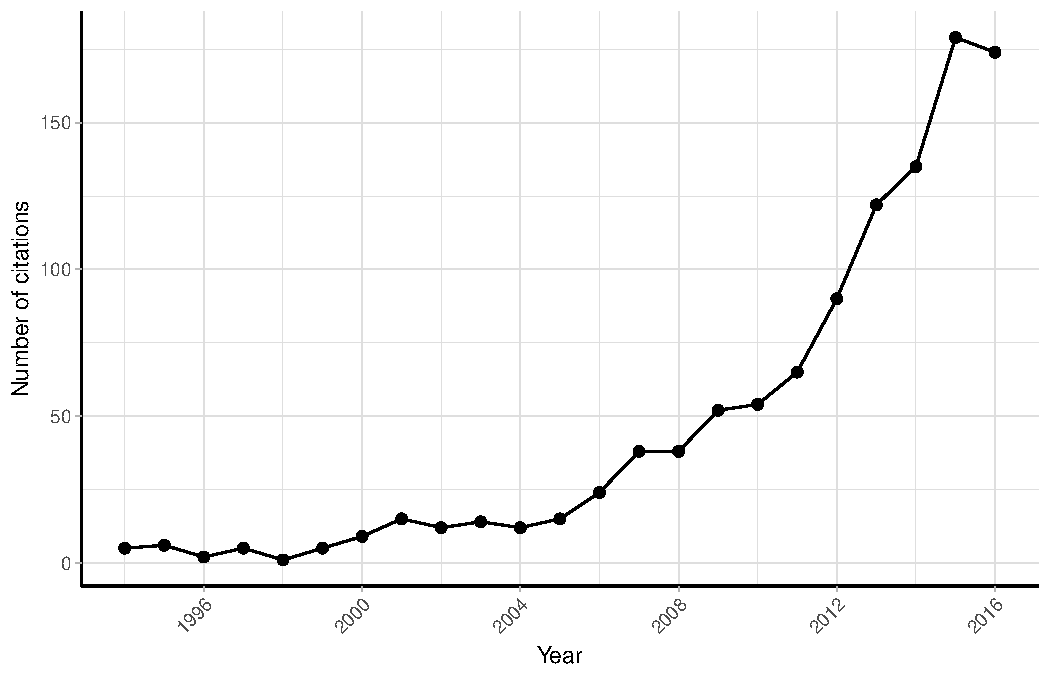
\includegraphics[width=\textwidth]{../figure/cite_grl-1} 

}

\caption[Number of citations of the paper by Greenland and Longnecker (1992) obtained from Google Scholar 1992-2017 (until December 2017)]{Number of citations of the paper by Greenland and Longnecker (1992) obtained from Google Scholar 1992-2017 (until December 2017).}\label{fig:cite_grl}
\end{figure}


\end{knitrout}

The common approach for dose--response meta-analysis consists of a two-stage procedure, where the regression coefficients for the study-specific trends are first estimated separately within each study, and then combined using meta-analysis. In the next sections we cover the main methodological aspects related to each stage of the analysis.


\subsection{First stage: study-specific trends}\label{sec:1st_stage}

If we had access to the individual patient data, the dose--response model for a simple linear trend could be written as
\begin{equation}
\log \left( \lambda \left(x, \mathbf{z} \right) \right) =  \beta_0 + \beta_1x + \boldsymbol{\gamma}^\top \mathbf{z}
\label{eq:lin_ipd}
\end{equation}
\noindent with $x$ is the quantitative exposure and $z$ the set of possible confounders. The outcome variable is the log of a transformation of the mean outcome (e.g. odds, risk, or rate). Transformations of the exposure variable can be included to relax the linearity assumption, such as a quadratic term
\begin{equation}
\log \left( \lambda \left(x, \mathbf{z} \right) \right) =  \beta_0 + \beta_1x + \beta_2x^2 + \boldsymbol{\gamma}^\top \mathbf{z}
\label{eq:quadr_ipd}
\end{equation}
\noindent However, we have rarely access to the individual patient data and our inference is limited to a summary of the initial data. In particular, aggregated data from a categorical analysis can be often retrieved from published articles. 
\noindent The aim of the first stage of a dose--response meta-analysis is to estimate the $\beta$ coefficients in Equation~\ref{eq:lin_ipd} and \ref{eq:quadr_ipd} using aggregated dose--response data. We consider the notation presented in Table~\ref{tab:aggr_data} with $i = 1, \dots, I$ indexing the studies and $j = 1, \dots, J_i$ the non-referent dose levels of a generic $i$-th study. The corresponding two models can be written as
\begin{equation}
\log \left( \widehat{\mathrm{RR}}_{ij} \right) = \log \left( \hat \lambda \left(x = x_{ij} \right) \right) - \log \left( \hat \lambda \left(x = x_{i0} \right) \right) = \beta_1\left(x_{ij} - x_{i0} \right)
\label{eq:lin_ad}
\end{equation}
\begin{equation}
\log \left( \widehat{\mathrm{RR}}_{ij} \right) = \log \left( \hat \lambda \left(x = x_{ij} \right) \right) - \log \left( \hat \lambda \left(x = x_{i0} \right) \right) = \beta_1\left(x_{ij} - x_{i0} \right) + \beta_2\left(x_{ij}^2 - x_{i0}^2 \right)
\label{eq:quadr_ad}
\end{equation}

\noindent More generally, the $i$-th dose--response model is defined as
\begin{equation}
\mathbf{y}_i = \mathbf{X}_i \boldsymbol{\beta}_i + \boldsymbol{\varepsilon}_i
\label{eq:drmodel}
\end{equation}
The outcome $\mathbf{y}_i$ is the $J_i$ length vector of the non-referent log $\widehat{\mathrm{RR}}$s while $\mathbf{X}_i$ the $J_i \times p$ design matrix containing the $p$ transformations of the assigned dose used to model the dose--response association
\begin{equation}
 \mathbf{X}_i=\left[
\begin{array}{ccc}
g_{1}(x_{i1}) - g_{1}(x_{i0}) & \hdots & g_{p}(x_{ip}) - g_{p}(x_{i0}) \\
\vdots &  & \vdots \\
g_{1}(x_{iJ_i}) -  g_{1}(x_{i0}) & \hdots & g_{p}(x_{iJ_i}) -  g_{p}(x_{i0}) \\
\end{array}%
\right] 
\label{eq:des.matrix}
\end{equation}

\noindent In the linear trend analysis (model~\ref{eq:lin_ad}), $\mathbf{X}_i$ includes only the dose levels, $p$ = 1, $g_1(x) = x$ (identity function)

\begin{equation*}
 \mathbf{X}_i=\left[
\begin{array}{c}
x_{i1} - x_{i0} \\
\vdots \\
x_{iJ_i} - x_{i0} \\
\end{array}%
\right] 
\end{equation*}

\noindent while $p = 2$ columns are needed in the quadratic model ~\ref{eq:quadr_ad}: $g_1(x) = x$ and $g_2(x) = x^2$

\begin{equation*}
 \mathbf{X}_i=\left[
\begin{array}{cc}
x_{i1} - x_{i0} & x_{i1}^2 - x_{i0}^2 \\
\vdots & \vdots \\
x_{iJ_i} - x_{i0} & x_{iJ_i}^2 - x_{i0}^2 \\
\end{array}%
\right] 
\end{equation*}

\noindent A feature of the models \ref{eq:drmodel} is the absence of the intercept term. The reference line in Table~\ref{tab:aggr_data} is not actually used for the estimation of the regression coefficients but introduces the constrain on the predicted log $\widehat{\mathrm{RR}}$, which needs to be 0 ($\widehat{\mathrm{RR}}$ = 1) for the reference dose value $x_{i0}$, as explicit in models~\ref{eq:lin_ad} and~\ref{eq:quadr_ad}.

\subsubsection*{Approximation of the covariance between log $\widehat{\mathrm{RR}}$}\label{sec:cov}

\noindent A particular characteristic of summarized dose--response data is that the log $\widehat{\mathrm{RR}}$s are reported with different precision and are constructed using the same baseline group. Thus, the error terms $\boldsymbol{\varepsilon}_i$ in Equation~\ref{eq:drmodel} are heterogeneous and correlated, with a covariance matrix structured as
\begin{equation}
\Cov\left(\boldsymbol{\epsilon}_i\right) = \mathbf{S}_i = \left[
\begin{array}{ccccc}
\sigma_{i11} & \ \ & \ & & \ \\
\vdots \ & \ddots & & & \ \\
\sigma_{i1j}& \ & \sigma_{ijj}& & \ \\
\vdots & \ & \ & \ddots & \\
\sigma_{i1J_i} & \ldots & \sigma_{iJ_ij} & \ldots & \sigma_{iJ_iJ_i}
\end{array}
\right] 
\label{eq:S_i}
\end{equation}
\noindent with the variance of the log $\widehat{\mathrm{RR}}$s on the diagonal ($\sigma_{ijj}$) and the pairwise covariances as non-diagonal elements ($\sigma_{ijj'}$).

\noindent Two methods have been proposed to approximate the covariances $\sigma_{ijj'}$ \citep{greenland1992methods, hamling2008facilitating}. Greenland and Longnecker described an algorithm to construct a table of pseudo or effective counts (number of cases and participants or person-time) that would produce the adjusted log $\widehat{\mathrm{RR}}$s as those published. A unique solution for the algorithm is ensured by keeping the margins of the pseudo-counts equal to the observed ones. Alternatively, Hamling et al. modified the previous algorithm in such a way that the pseudo-counts would also match the standard errors of the log $\widehat{\mathrm{RR}}$s. 

\subsubsection*{Estimation}

The dose--response coefficients $\boldsymbol{\beta}_i$ can be efficiently estimated using generalized least squares estimator (GLS), which minimizes the quadratic loss function $\left(\mathbf{y}_i- \mathbf{X}_i \boldsymbol{\beta}_i \right)^\top \mathbf{S}_i^{-1} \left(\mathbf{y}_i- \mathbf{X}_i \boldsymbol{\beta}_i \right)$ with respect to $\boldsymbol{\beta}_i$ assuming the covariance matrix $\mathbf{S}_i$ known
\begin{equation}
\begin{gathered}
\boldsymbol{\hat \beta}_i = ( \mathbf{X}_i^\top  \mathbf{S}_i^{-1} \mathbf{X}_i)^{-1} \mathbf{X}_i^\top  \mathbf{S}_i^{-1} \mathbf{y}_i \\ 
\widehat{\Var} \left( \boldsymbol{\hat \beta}_i \right) = ( \mathbf{X}_i^\top \mathbf{S}_i^{-1} \mathbf{X}_i)^{-1}
\end{gathered}
\label{eq:gls}
\end{equation}

\noindent The GLS estimates in Equation~\ref{eq:gls} do not require any distributional assumption for the error terms. However, for the central limit theory, the error terms follow approximately a normal distribution $\boldsymbol{\epsilon}_i \sim \mathcal{N}\left(\mathbf{0}, \mathbf{S}_i \right)$. 
Using this additional assumption, the log-likelihood of model~\ref{eq:drmodel} is
\begin{equation}
\ell\left(\boldsymbol{\beta}_i\right) = -\frac{J_i}{2}\log\left(2\pi\right) - \frac{1}{2}\log|\mathbf{S}_i| - \frac{1}{2} \left[\left(\mathbf{y}_i- \mathbf{X}_i \boldsymbol{\beta}_i \right)^\top \left( \mathbf{S}_i \right)^{-1} \left(\mathbf{y}_i- \mathbf{X}_i \boldsymbol{\beta}_i \right) \right]
\label{eq:drmodel_logLik}
\end{equation}

\noindent Interestingly, the maximum likelihood (ML) estimates that maximize the log-likelihood~\ref{eq:drmodel_logLik} coincides with the GLS estimates in~\ref{eq:gls} \citep{orsini2006generalized}. Introducing the normality distribution for the random errors facilitates the inference, i.e. test of hypothesis and confidence intervals, on the $\boldsymbol{\beta}_i$ coefficients. The estimates in~\ref{eq:gls} are a linear combination of normal distributions, $\mathbf{y}_i \sim \mathcal{N}\left(\mathbf{X}_i \boldsymbol{\beta}_i, \mathbf{S}_i \right)$, and therefore are also normally  distributed $\boldsymbol{\hat \beta}_i \sim \mathcal{N}\left( \boldsymbol{\beta}_i, {\Var} \left( \boldsymbol{\hat \beta}_i \right)\right)$.

The ML and GLS estimators give unbiased estimates of $\boldsymbol{\beta}_i$ regardless of the specification of $\mathbf{S}_i$ \citep{orsini2006generalized}. As a consequence, also a weighted least squares estimator (WLS) that assumes independence of the log $\widehat{\mathrm{RR}}$s will produce unbiased estimates. However, taking into account the correlation will improve the statistical properties of the estimator, in particular the efficiency. 
We investigated the differences between the GLS and WLS estimators using a simulation study of 5000 aggregated dose--response data where the true trends were linear ($\beta_\text{TRUE} =$ -0.014). As expected, both the estimators were unbiased and consistent but the empirical distribution of the GLS estimator was more concentrated around the true $\beta$ value \ref{fig:cov_methods_lin}. The WLS estimates of the standard errors of the $\hat \beta_i$ were lower than the corresponding GLS values. This had a direct effect on the inference for the estimated linear trend. For instance, it may be interesting to fit a quadratic curve as in~\ref{eq:quadr_ad} and test the hypothesis $H_0: \beta_2 = 0$, i.e. departure from a linear trend. Using inference based on WLS estimators the null hypothesis were wrongly rejected 3.96\% of the time, lower than the nominal level $\alpha = 5$\%. The corresponding number for the GLS estimator was instead closer (4.8\%). 
\noindent We also implemented simulations assuming a quadratic curve with the true coefficients $\boldsymbol{\beta}_\text{TRUE}$ = (-0.092, 0.003). Similar results for the empirical bivariate distribution of $ \boldsymbol{\hat \beta}_i$ and their standard errors are presented in Figure~\ref{fig:cov_methods_quadr}.

\begin{knitrout}\footnotesize
\definecolor{shadecolor}{rgb}{1, 1, 1}\color{fgcolor}\begin{figure}[ht!]

{\centering \includegraphics[width=\textwidth]{../figure/cov_methods_lin-1} 

}

\caption[Empirical distribution of the $\hat \beta$ (panel A) and $\widehat{\Var} \left( \hat \beta_i \right)$ (panel B) for a linear trend assuming independence of the log $\widehat{\mathrm{RR}}$  and reconstructing the covariances using the Greenland and Longnecker’s method]{Empirical distribution of the $\hat \beta$ (panel A) and $\widehat{\Var} \left( \hat \beta_i \right)$ (panel B) for a linear trend assuming independence of the log $\widehat{\mathrm{RR}}$  and reconstructing the covariances using the Greenland and Longnecker’s method. Results are based on simulations with 5000 replications and a true linear trend $\beta = $-0.014.}\label{fig:cov_methods_lin}
\end{figure}


\end{knitrout}

\begin{knitrout}\footnotesize
\definecolor{shadecolor}{rgb}{1, 1, 1}\color{fgcolor}\begin{figure}[ht!]

{\centering \includegraphics[width=\textwidth]{../figure/cov_methods_quadr-1} 

}

\caption{Empirical bivariate distribution of the beta coefficients (panel A) and their standard errors (panel B) for a quadratic trend assuming independence of the log $\widehat{\mathrm{RR}}$  and reconstructing the covariances using the Greenland and Longnecker’s method. Results are based on simulations with 5000 replications and a true quadratic trend $\beta_{1} = $-0.092, $\beta_{2} = $0.003.}\label{fig:cov_methods_quadr}
\end{figure}


\end{knitrout}


\subsection{Second stage: multivariate meta-analysis}\label{sec:2nd_stage}

The study-specific dose--response curves are defined by the $p$ transformations, $g_1(x), \dots, g_p(x)$, and the estimated regression coefficients $\boldsymbol{\hat \beta}_i$. A pooled dose--response can be obtained by combining the $\boldsymbol{\hat \beta}_i$ coefficients. For that purpose, the same functional relationship needs to be defined across the studies. Therefore, the transformations of the exposure were not subscripted by the study index $i$.

\noindent The $p$ length vector of the $\boldsymbol{\hat \beta}_i$ parameters and the accompanying $p \times p$ covariances matrices $\widehat{\Var} \left( \boldsymbol{\hat \beta}_i \right)$ serve as outcome in the meta-analytic model. We consider the setting with $p \ge 2$ and relate the univariate case as a simpler instance of the more general multivariate case. Since the dimension of the outcome is no longer univariate, extensions of models \ref{eq:rma} to the multivariate settings can be implemented for accommodating the synthesis of correlated estimates \citep{berkey1998meta, gasparrini2012multivariate, ritz2008multivariate}.

\subsubsection*{Model definition}

A multivariate random-effects model has a similar formulation as in the univariate case
\begin{equation}
\boldsymbol{\hat \beta}_i = \boldsymbol{\beta} + \mathbf{b}_i + \boldsymbol{\varepsilon}_i
\label{eq:rmma}
\end{equation}
\noindent The unobserved random effects $\mathbf{b}_i$ are now of dimension $p$, still representing study-specific deviation from the mean $\boldsymbol{\beta}$ parameter. As before, they have zero mean $\E\left[\mathbf{b}_i\right] = \mathbf{0}$ and $\Var\left[\mathbf{b}_i\right] = \boldsymbol{\Psi}$, the $p \times p$ between-study variance matrix. Specification of a parametric distribution for the random-effects may facilitate the inference (especially confidence intervals) and improve the prediction of marginal and conditional dose--response associations. Typically a multivariate normal distribution is adopted $\mathbf{b}_i \sim \mathcal{N}\left(\mathbf{0}, \boldsymbol{\Psi} \right)$. Hence, we can write the marginal model of~\ref{eq:rmma} as
\begin{equation}
\boldsymbol{\hat \beta}_i \sim \mathcal{N}\left(\boldsymbol{\beta}, \boldsymbol{\Sigma}_i \right)
\label{eq:rmma2}
\end{equation}
\noindent where the marginal variance $\boldsymbol{\Sigma}_i = \widehat{\Var} \left( \boldsymbol{\hat \beta}_i \right) + \boldsymbol{\Psi}$ is defined by the sum of the within-study and between-studies variance components. The model~\ref{eq:rmma2} implies a two-stage sampling procedure where the study-specific $\boldsymbol{\beta}_i$ parameters are assumed to be sampled from a multivariate normal distribution centered around the population average parameter $\boldsymbol{\beta}$. The study-specific estimates $\boldsymbol{\hat \beta}_i$ are themselves sampled from a multivariate distribution with zero mean and error variance assumed known.

\noindent The multivariate random-effects model~\ref{eq:rmma2} can be extended to meta-regression models by including study-levels covariates that might change the shape of the dose--response relationship. The dose--response coefficients are then modeled as a linear combination of the $m$ study-level covariates $\mathbf{u}_i = \left(u_{i1}, \dots, u_{im} \right)$, with $u_{i1} = 1$ representing the intercept term
\begin{equation}
\boldsymbol{\hat \beta}_i \sim \mathcal{N}\left(\widetilde{\mathbf{X}}_i \boldsymbol{\beta}, \boldsymbol{\Sigma}_i\right)
\label{eq:rmmra2}
\end{equation}
\noindent The $p\times pm$ design matrix $\widetilde{\mathbf{X}}_i$ is constructed taking the Kronecker product between the $\mathbf{u}_i$ and the identity matrix of dimension $p$, $\mathbf{I}_{(p)}$
\begin{equation}
\widetilde{\mathbf{X}}_i = \mathbf{I}_{(p)} \otimes \mathbf{u}_i^\top = 
	\begin{bmatrix}
		1 & u_{i2} & \cdots & u_{im} & \cdots & 0 & 0 & \cdots & 0 \\
		\vdots &  &  &  & \ddots & &  &  &  \\
		0 & 0 & \cdots & 0 & \cdots & 1 & u_{i2} & \cdots & u_{im} \\
	\end{bmatrix}
\end{equation}
\noindent For example, the $\widetilde{\mathbf{X}}_i$ matrix relating the effect of a binary variable $u_i$ to the dose--response coefficients for a quadratic trend is
\begin{equation*}
\widetilde{\mathbf{X}}_i = \mathbf{I}_{(2)} \otimes \mathbf{u}_i^\top = 
	\begin{bmatrix}
		1 & 0 \\
		0 & 1
	\end{bmatrix} \otimes
	(1, u_i)=
	\begin{bmatrix}
		1 & u_i  & 0 & 0 \\
		0 & 0 & 1 & u_i  \\
	\end{bmatrix}
\end{equation*} 

\noindent The dimension of $\boldsymbol{\hat \beta}$ is now $p\times m$. The coefficients related to the intercept terms are interpreted as the mean dose--response coefficient when all the study-level covariates $\mathbf{u}$ are equal to zero. The remaining coefficients indicate how the mean dose--response association vary with respect to the corresponding study-level covariate.


\subsubsection*{Estimation}

Several methods are available for estimating the parameters of interest, namely the $p \times m$ dose--response coefficients in $\boldsymbol{\beta}$ and the $p(p+1)/2$ length vector $\boldsymbol{\xi}$ containing the elements of the between-studies covariance $\boldsymbol{\Psi}$. There is generally no reason to assume a specific covariance structure \citep{white2011multivariate}. We consider here likelihood-based estimators \citep{verbeke1997linear, pinheiro2010mixed}. In particular, ML estimators estimate simultaneously $\boldsymbol{\beta}$ and $\boldsymbol{\xi}$ by maximizing the log-likelihood of the marginal model~\ref{eq:rmmra2}
\begin{equation}
\ell\left(\boldsymbol{\beta}, \boldsymbol{\xi} \right) = -\frac{1}{2}Ip\log(\pi) -\frac{1}{2}\sum_{i=1}^I \log |\boldsymbol{\Sigma}_i| - \frac{1}{2}\sum_{i=1}^I\left[ \left(\boldsymbol{\hat \beta}_i - \widetilde{\mathbf{X}}_i\boldsymbol{\beta} \right)^\top \boldsymbol{\Sigma}_i^{-1} \left(\boldsymbol{\hat \beta}_i - \widetilde{\mathbf{X}}_i\boldsymbol{\beta} \right) \right]
\label{eq:rmma_logLik}
\end{equation}

\noindent ML estimators, however, don’t take into account the loss of degrees of freedom due to the $\boldsymbol{\beta}$ estimation \cite{harville1977maximum}. Alternatively, restricted maximum likelihood methods (REML) maximizes a set of contrasts defined as a function of the only covariance parameters
\begin{equation}
\begin{split}
\ell_R\left(\boldsymbol{\xi} \right) =& -\frac{1}{2}\left(Ip - pm\right) -\frac{1}{2}\sum_{i=1}^I \log |\boldsymbol{\Sigma}_i| -\frac{1}{2}\sum_{i=1}^I \log \left|\widetilde{\mathbf{X}}_i^\top\boldsymbol{\Sigma}_i\widetilde{\mathbf{X}}_i \right| + \\
&- \frac{1}{2}\sum_{i=1}^I\left[ \left(\boldsymbol{\hat \beta}_i - \widetilde{\mathbf{X}}_i\boldsymbol{\beta} \right)^\top \boldsymbol{\Sigma}_i^{-1} \left(\boldsymbol{\hat \beta}_i - \widetilde{\mathbf{X}}_i\boldsymbol{\beta} \right) \right]
\end{split}
\label{eq:rmma_logRLik}
\end{equation}

\noindent Both estimation methods require iterative algorithms, where conditional estimates of $\boldsymbol{\hat \beta}$ are plugged in either \ref{eq:rmma_logLik} or \ref{eq:rmma_logRLik}, regarded as function of $\boldsymbol{\xi}$ only, until convergence. More details on the implementation of iterative methods for maximizing Equations~\ref{eq:rmma_logLik} and ~\ref{eq:rmma_logRLik} are described by \cite{gasparrini2012multivariate}.


\subsubsection*{Hypothesis testing, heterogeneity, and model comparison}

There are two main domains of interest for making inference that relate either to the fixed-effects $\boldsymbol{\beta}$ or the variance components in $\boldsymbol{\Psi}$. Using the normality assumption for the random-effects, inference is based on the approximated normal distribution for $\boldsymbol{\hat \beta}$, with mean and covariance matrix defined similarly as in Equation~\ref{eq:gls}.

\noindent Since the mean dose--response association is defined by the $\boldsymbol \beta$, the hypothesis of no association can be evaluated by testing $H_0: \boldsymbol{\beta} = \boldsymbol{0}$. 
%In case of $p > 1$ multivariate Walt-type test are needed.
Alternatively, a subset or linear combinations of the elements in $\boldsymbol \beta$ may be of interest. For example, in a quadratic trend the non-linearity is introduced by the quadratic term $x^2$. Thus, testing $H_0: \beta_2 = 0$ is a possible way for evaluating departure from a linear dose--response relationship.

As previously presented in section~\ref{sec:het_rma}, the coefficients defining $\boldsymbol{\Psi}$ are not nuisance parameters rather than useful for quantifying the variation of the study-specific associations $\boldsymbol{\beta}_i$. Similar measures for testing and quantifying the impact of heterogeneity have been extended to the multivariate setting \citep{berkey1996multiple}. In particular, the $Q$~statistic
\begin{equation}
Q = \sum_{i=1}^I \left(\boldsymbol{\hat \beta}_i - \widetilde{\mathbf{X}}_i\boldsymbol{\hat \beta}_{\text{fe}}\right) ^\top \widehat{\Var} \left( \boldsymbol{\hat \beta}_i \right)^{-1} \left(\boldsymbol{\hat \beta}_i - \widetilde{\mathbf{X}}_i\boldsymbol{\hat \beta}_{\text{fe}}\right)
\label{eq:Qmulti}
\end{equation}
\noindent with $\boldsymbol{\hat \beta}_{\text{fe}}$ estimated under a fixed-effect model is used to test $H_0: \boldsymbol{\Psi} = \boldsymbol{0}$. Under the null hypothesis, the $Q$~statistic follow a $\chi^2$ with $Ip - pm$ degrees of freedom. When $p = 1$ the formulations~\ref{eq:Q} and~\ref{eq:Qmulti} coincide. The multivariate extension of the $I^2$ was derived relating the $Q$~statistics to its degrees of freedom $I^2 = \max \left\{0, \frac{Q- (Ip - pm)}{Ip - pm}\right\}$ \citep{jackson2012quantifying}.

The fit of alternative non-nested meta-analytical models can be compared using information criteria indeces such the Akaike information criterion (AIC), which is defined as $\textrm{AIC} = -2 \ell\left(\boldsymbol{\beta}, \boldsymbol{\xi} \right) + 2k$, a descriptive measure depending on the maximum log-likelihood and $k$, the number of estimated parameters. It is worth to note that the AIC can be used for comparing the fit of different analyses such as alternative meta-regression models. However, there is no reason to employ these indeces, derived from the meta-analytic models, for comparing different dose--response models, such as linear vs non-linear. 


\subsubsection*{Prediction}\label{sec:pred}

Oftentimes the estimated mean coefficients $\boldsymbol{\hat \beta}$ are not directly interpretable (an exception is the estimate for a linear trend). The dose--response results are thus communicated as predicted (log) relative risk for selected exposure levels using one value as referent. Obtaining predictions either in a graphical or tabular presentation is thus an important step of the analysis and yet often poorly implemented.
Based on the model~\ref{eq:rmma}, the predicted $\log RR$ for a dose level $x_v$ using $x_\mathrm{ref}$ as referent can be calculated as
\begin{align}
\log \widehat{RR}(x = x_v) = \mathbf{X}_v\boldsymbol{\hat \beta} \label{eq:pred} \\
\Var \left(\log \widehat{RR}(x = x_v) \right) = \mathbf{X}_v \widehat{\Var} \left( \boldsymbol{\hat \beta} \right) \mathbf{X}_v^\top \label{eq:varpred}
\end{align}
\noindent where $\mathbf{X}_v$ is the design matrix evaluated in $x_v$, as defined in the first-stage analysis (Equation~\ref{eq:des.matrix}). For example, the predicted $\log RR$ for the quadratic model~\ref{eq:quadr_ad} comparing $x_v$ versus $x_\mathrm{ref}$ is
\begin{equation*}
\log \widehat{RR}(x = x_v) = \hat \beta_1 \left(x_v - x_\mathrm{ref} \right) + \hat \beta_2 \left(x_v^2 - x_\mathrm{ref}^2 \right)
\end{equation*}
Of note, the referent dose $x_\mathrm{ref}$ is an arbitrary value and thus does not need to correspond to any of the study-specific reference values $x_{i0}$.

\noindent A confidence interval for the predicted $\log \widehat{RR}(x = x_v)$ is based on the normal distribution of $\boldsymbol{\hat \beta}$
\begin{equation*}
\log \widehat{RR}(x = x_v) \mp z_{1- \alpha/2} \Var \left(\log \widehat{RR}(x = x_v) \right)^{\frac{1}{2}}
\label{eq:pred_ci}
\end{equation*}

\noindent Formulas~\ref{eq:pred} and~\ref{eq:varpred} can be extended to meta-regression models. The predicted $\log RR$ conditional on a specific study-level covariate pattern $\mathbf{u} = \mathbf{u}_v$ is
\begin{align}
\log \widehat{RR}\left(x = x_v, \mathbf{u} = \mathbf{z}_v  \right)= \mathbf{X}_v \left(\mathbf{I}_{(p)} \otimes \mathbf{U}_v^\top \right) \boldsymbol{\hat \beta}  \label{eq:pred_mr} \\
\Var \left(\log \widehat{RR}\left(x = x_v, \mathbf{z}= \mathbf{z}_v \right) \right) = \left( \mathbf{X}_v \mathbf{U}_v\right) \widehat{\Var} \left( \boldsymbol{\hat \beta} \right) \left( \mathbf{X}_v \mathbf{U}_v\right)^\top \label{eq:varpred_mr}
\end{align}

Inference on study-specific dose--response associations can be enhanced by exploiting the information from the multivariate distribution for the random-effects. The best linear unbiased prediction (BLUP) for the study-specific regression coefficients $\mathbf{b}_i$ are defined as
\begin{equation}
\boldsymbol{\hat b}_i = \boldsymbol{\Psi} \boldsymbol{\Sigma}_i^{-1} \left(\boldsymbol{\hat \beta}_i - \widetilde{\mathbf{X}}_i \boldsymbol{\hat \beta} \right)
\label{eq:blup_ts}
\end{equation}
\noindent Study-specific predicted log relative risks can be obtained as in Equations~\ref{eq:pred} and~\ref{eq:varpred} by replacing the mean parameter $\boldsymbol{\hat \beta}$ with the individual dose-response coefficients $\boldsymbol{\hat \beta} + \boldsymbol{\hat b}_i$ 


\subsection{Methodological research}

Dose--response meta-analysis has received attention not only in applied works but also in theoretical articles that covered different aspects of the methodology. 
\noindent \cite{greenland1992methods} originally presented the two-stage approach for efficiently estimating a linear trend in a fixed-effect analysis. An alternative model for estimating curvilinear model, referred to as ``pool first'', was also presented. The technique consists of a one-stage approach where the aggregated data are considered altogether and a single model as in~\ref{eq:drmodel} is fitted. By first combining the data, more flexible curve parametrized by multiple parameters ($p \ge 2$) can be estimated. The study-specific dose--response analyses are limited by the minimum number of non-referent log RRs across the studies. For example, if the aggregated data for a study consists of only one non referent log RR, only a univariate model with $p = 1$ can be estimated. The authors refined the methodology by extending the two-stage approach to allow for heterogeneity limited to a linear trend analysis \citep{berlin1993meta}. 

\subsubsection*{Flexible dose--response models}

The primary interest of the methodological research was in presenting alternative strategies for estimating non-linear curves. \cite{bagnardi2004flexible} described the use of fractional polynomials and restricted cubic splines using aggregated dose--response data. Based on a practical example on the association between alcohol consumption and all-cause mortality, the authors showed how implementation of these flexible techniques may prevent misleading results from conventional polynomials (e.g. quadratic) curves. 
Second-degree fractional polynomials (FP2) consist of a large family of curves defined in the general form of
\begin{equation}
\mathrm{FP2}(x) = \beta_1 x^{p_1} + \beta_2x^{p_2}
\label{eq:fracpol}
\end{equation}
\noindent where $p_1$ and $p_2$ are chosen in the set of power coefficients $\left\{-2, -1, -0.5, 0, 0.5, 1, 2, 3 \right\}$ \citep{royston1994regression, royston2000strategy}. When $p = 0$, $x^p$ becomes $\log(x)$, while if $p_1 = p_2$ the second transformation of $x$ becomes $x^{p_2}\log(x)$. The advantage of FP2 models is that different shapes, including U- and J-shapes, can be estimated by only two coefficients chosen using different combinations for the power terms $(p_1, p_2)$. Typically, the best fitting fractional polynomial is chosen in such a way that the $(p_1, p_2)$ corresponds to the model with the highest likelihood, or equivalently, lowest deviance \citep{royston2001flexible}. 

A popular alternative for flexibly model the dose--response association is represented by the use of splines \citep{de1978practical}, largely presented by \cite{orsini2011meta} using data from the Pooling Project of Prospective Studies of Diet and Cancer. Splines functions consist of consecutive polynomials connected at specific points of the exposure range called knots. Choosing $\mathbf{k} = \left(k_1, \dots, k_K\right)$ knots and third order polynomials, the model, also known as cubic splines (CS), is defined as
\begin{equation}
\mathrm{CS}(x) = \beta_1 x + \beta_2x^2 + \beta_3x^3 + \sum_{l = 1}^{K-1} \beta_{l+3}(x - k_l)_{+}^3
\label{eq:cs}
\end{equation}
\noindent where the `+' notation has been used ($u_+ = u$ if $u \ge 0$ and $u_+ = 0$ otherwise). To avoid strange behaviors at the extremes of the exposure range, the model~\ref{eq:cs} is constrained to be linear before and after the first and last knots, respectively. For example, using the minimum number of three knots a restricted cubic spline model (RCS) can be specified in terms of two coefficients
\begin{equation}
\mathrm{RCS}(x) = \beta_1 x + \beta_2 \left[ \left( x - k_1 \right)_{+}^3 - \frac{k_3 - k_1}{k_3 - k_2} \left( x - k_2  \right)_{+}^3 + \frac{k_2 - k_1}{k_3 - k_2} \left(x - k_3 \right)_{+}^3\right]
\label{eq:rcs}
\end{equation}
\noindent The second transformation is generally divided by $(k_3 - k_1)^2$ to improve the numerical behavior and to put the spline transformations on the same scale \citep{harrell2015regression} (see Appendix~\ref{sec:rcs} for the derivation of a RCS model).

The previous strategies have been often presented for exposures where 0 was the natural reference categories (e.g. alcohol consumption). \cite{liu2009two} extended the methodology for handling non-zero reference categories, as in the case of Body Mass Index. In particular, they first described how to construct the design matrix in terms of contrasts, as clarified in Equation~\ref{eq:des.matrix}. Misspecification of the design matrix (e.g. $\log \mathrm{RR} = \beta_1 (x_1 - x_0) + \beta_2 (x_1 - x_0)^2$ instead of $\log \mathrm{RR} = \beta_1 (x_1 - x_0) + \beta_2 (x_1^2 - x_0^2)$) may increase the risk of generating artifacts and misleading conclusions. Note that for zero exposure categories the problem is generally not relevant since many functions return zero for $x = 0$ ($g(0) = 0$).

\subsubsection*{Multivariate meta-analysis}

The major contribution for estimating non-linear curves in a random-effects analysis came with the extension of univariate meta-analytic models to the multivariate case. The formalization and implementation of multivariate meta-analysis enabled the extension of a two-stage dose--response meta-analysis to the more complex case of multiple parameters association \citep{gasparrini2012multivariate}. The multivariate framework can accommodate the synthesis of correlated outcomes or estimates, as those derived in the first stage of a dose--response meta-analyses. The application of the strategies presented in~\ref{eq:fracpol} and~\ref{eq:rcs} in a random-effects setting has been easily facilitated by the implementation of dedicated packages for multivariate meta-analysis \citep{white2011multivariate, jackson2011multivariate}. This is probably the reason why a one-stage approach for dose--response meta-analysis was no further extended.

\noindent The methodological advancements for meta-analysis were diverse and numerous (see \cite{sutton2008recent} for an overview). Important improvements that directly affected how results are presented related mainly to the quantification and assessment of heterogeneity, with the definition of the measures presented in section~\ref{sec:het_rma}. In addition, many other articles enriched the set of tools for pooling study-specific effects, with a direct application to the second stage of a dose--response meta-analysis. Among the many, it is worth to mention the implementation of several estimation methods for the between-study variability (see \cite{langan2017comparative} for a comparison based on simulation studies); advancement in performing meta-regression \citep{van2002advanced}; proposal of sequential approaches \citep{pogue1997cumulating} and statistical power \citep{sutton2007evidence}; and introduction of Bayesian methods \citep{sutton2001bayesian}.

\subsubsection*{Covariance and sensitivity analysis}

\cite{orsini2006generalized} refined the initial formulas presented by Greenland and Longnecker for approximating the study-specific covariance matrices depending on the study-design. \cite{berrington2003generalized} described an alternative method that avoids the reconstruction of the covariance matrices. Instead, upper and lower bounds for the covariance matrix are used in a sensitivity analysis of the dose--response coefficients, adopting a range of plausible values for the covariances. While the alternative algorithm proposed by \cite{hamling2008facilitating} was presented in section~\ref{sec:cov}, \cite{easton1991floating} proposed the implementation of the floating absolute risks where the parameters and their standard errors can be estimated without specifying a baseline group and thus can be regarded as independent. Using individual patient data from the Pooling Project of Prospective Studies of Diet and Cancer (\url{http://www.hsph.harvard.edu/poolingproject}), negligible differences in the reconstructed covariance matrices were found comparing the three approaches \citep{orsini2011meta}. Of note, none of the methods would be needed if the authors of the original articles provided the covariance matrix along with the estimated coefficients, as it is usually done in consortia projects.

\cite{berlin1993meta} presented alternatives for assigning the dose levels within exposure categories and illustrated the use of meta-regression models for investigating the possible effect of study-level characteristics on the estimated linear trends. \cite{shi2004meta} further discussed the issue of dose assignment in grouped measures allowing for arbitrary dose levels. In addition, they investigated the effect of heterogeneity and publication bias by means of sensitivity analyses. A similar problem of dose assignment was addressed by using a likelihood approach limited to a linear trend analysis \citep{takahashi2010assignment}. This idea has been further extended to the case of restricted cubic splines \citep{takahashi2013cubic}.

\subsection{Research questions}

There were still many open research questions that need to be addressed to improve the synthesis of aggregated dose--response data. It was useful to observe the current practice in applied works in order to identify the more relevant questions. We searched the PubMed database for articles published between January 1, 2013 and April 1, 2013 using the research query (``meta-analysis'' [Title] and ``dose-response'' [Title]) and, after excluding irrelevant articles, found 42 applied dose--response meta-analyses. The authors of the select articles conducted a linear trend analysis most of the times (25 times, 60\%) while only 17 articles considered non-linear associations by means of restricted cubic splines (15) and fractional polynomials (2). The papers modelling non-linear curves reported a graphical presentation of the pooled dose--response association.

\noindent Interestingly, none of the retrieved articles evaluated the goodness-of-fit of the selected dose--response model. The assessment of how the estimated curve fits the aggregated data should be a natural and important step in a dose--response analysis. In \citetalias{discacciati2015goodness} we will address this important issue by presenting relevant measures and graphical tools to help the assessment of goodness-of-fit.

\noindent The majority of the screened papers (39, 93\%) quantify the impact of heterogeneity by reporting results for the $Q$~test and the value of $I^2$. While the limitations of the $Q$~test approach are widely known, little emphasis is placed on the assumptions underneath the definition of the established measures of heterogeneity, i.e.  all the estimates being reported with the same precision, which is unlikely to be met in almost all the applications. A measure of the impact of heterogeneity that does not require such an assumption would be desirable. In \citetalias{crippa2016new} we overcome this limitation by proposing an alternative measure of heterogeneity and comparing the performance of the new and available measures.

\noindent None of the surveyed meta-analyses discussed the sensitivity of the overall dose--response relationship to differences in study-specific exposure distribution. This analysis can be very relevant in case of studies reporting results for heterogeneous exposure range. Application of a point-wise average approach originally presented by \cite{sauerbrei2011new} in the context of individual patient data may represent an interesting alternative to the averaging of regression coefficients. In \citetalias{crippa2018pointwise} we will evaluate the advantages of this strategy based on aggregated dose--response data.

\noindent In all the meta-analyses assessing departure from of linearity, the authors excluded those studies reporting less than two non-referent RRs. Indeed, a two-stage dose--response meta-analysis requires that all the models in the dose--response analysis are identifiable ($p \le \min\left(J_i\right)$). A one-stage approach would avoid that requirement. Such an approach is conceptually easier to understand, and more elegant from a statistical point of view. In addition, it allows investigation of much more flexible dose--response curves, that are not possible within the context of a traditional two-stage analysis. Aim of \citetalias{crippa2018one} is to describe implementation and advantages of a one-stage random-effects dose--response meta-analysis of aggregated data.

\begin{knitrout}\footnotesize
\definecolor{shadecolor}{rgb}{1, 1, 1}\color{fgcolor}\begin{figure}[ht!]

{\centering \includegraphics[width=\textwidth]{../figure/dosresmeta_ts-1} 

}

\caption[Monthly number of downloads of the dosresmeta R package from the RStudio CRAN mirror September 2013 - December 2017]{Monthly number of downloads of the dosresmeta R package from the RStudio CRAN mirror September 2013 - December 2017.}\label{fig:dosresmeta_ts}
\end{figure}


\end{knitrout}



\section{Software}

Dissemination of new statistical methodologies is certainly facilitated by the development and implementation of statistical software components. Many theoretical papers have not been considered in applied works because of lack of user-friendly software. 

\noindent \cite{orsini2006generalized} described the \texttt{glst} command in Stata, the first publicly available procedure dedicated for dose--response meta-analysis. The command implements both the one- and two-stage approaches limited, in case of a random-effects analysis, to a linear trend. A two-stage random-effects meta-analysis of non-linear relationships can be performed with the aid of the \texttt{mvmeta} command for multivariate meta-analysis \citep{white2011multivariate}. Several worked examples and codes are available at \url{http://www.imm.ki.se/biostatistics/glst/}. Later on, \cite{li2010sas} wrote the macro \texttt{\%metadose}, a similar procedure for SAS users.
 
The majority of the applied meta-analyses retrieved in our survey were performed using the \texttt{glst} procedure in Stata (36, 87\%), while 2 used the \texttt{metadose} macro in SAS, 2 functions in RevMan. No dedicated package was available in the free software programming language \textsf{R}. Therefore, in 2013, we released the first version of the \pkg{dosresmeta} package on CRAN (\url{https://CRAN.R-project.org/package=dosresmeta}), a package specifically designed for dose--response meta-analysis in \textsf{R}, with specific functions that greatly facilitates the application in practical works. 

The \pkg{dosresmeta} package is now available in the updated version 2.0.1 and new features are being implemented in the version under development on GitHub (\url{https://github.com/alecri/dosresmeta}). Currently, the \pkg{dosresmeta} package is downloaded and used worldwide, with a median number of 260 downloads/month (Figure~\ref{fig:dosresmeta_ts}). The countries where it has been downloaded most are Great Britain (4005), United States (3905), and China (1605) (Figure~\ref{fig:dosresmeta_map}). Working examples, codes, and data are available at \url{http://alecri.github.io/software} for fully reproduce figures and numbers presented in both applied and theoretical papers.

\begin{knitrout}\footnotesize
\definecolor{shadecolor}{rgb}{1, 1, 1}\color{fgcolor}\begin{figure}[ht!]

{\centering \includegraphics[width=\textwidth]{../figure/dosresmeta_map-1} 

}

\caption[Total number of downloads of the doseresmeta R package worldwide from the RStudio CRAN mirror September 2013 - December 2017]{Total number of downloads of the doseresmeta R package worldwide from the RStudio CRAN mirror September 2013 - December 2017.}\label{fig:dosresmeta_map}
\end{figure}


\end{knitrout}

% !TeX root = ../kappa.Rnw  


% ---------------------------------------------------------
% Project: PhD KAPPA
% File: aims.tex
% Author: Alessio Crippa
% based on the template written by Andrea Discacciati
%
% Purpose: Aims
% ---------------------------------------------------------

\chapter{Aims of the thesis}

The overall aims of this thesis were to develop and implement new methods for dose--response in meta-analysis, in order to deal with the methodological aspects that have not yet been addressed.

\bigskip

More specifically, the aims were:

\begin{itemize}
\item To describe the implementation of the main aspects of a dose--response meta-analysis and the usage of the \pkg{dosresmeta} \textsf{R} package.

\item To present and discuss relevant measures and graphical tools to assess the goodness-of-fit in dose--response meta-analysis.

\item To develop a new measure of between-study heterogeneity in the broader context of meta-analysis and assess its properties as compared to other available measures. 

\item To explore possible advantages of a point-wise approach, especially, in case of dose--response meta-analysis where the exposure range varies substantially across the studies.

\item To formalize and present an alternative one-stage random-effects model for dose--response meta-analysis of aggregated data, formulating the meta-analytic model in terms of a general linear mixed-effect model. 

\end{itemize}

% !TeX root = ../kappa.Rnw  

% ---------------------------------------------------------
% Project: PhD KAPPA
% File: materials.tex
% Author: Alessio Crippa
% based on the template written by Andrea Discacciati
%
% Purpose: Materials
% ---------------------------------------------------------

\chapter{Methods}

\section{The \pkg{dosresmeta} \textsf{R} package}

The first version of the \pkg{dosresmeta} $\R$ package was released on the Comprehensive R Archive Network (CRAN) on September 9, 2013. It is listed in the CRAN task view Meta-Analysis (\url{https://CRAN.R-project.org/view=MetaAnalysis}), a guide that covers the vast collection of $\R$ packages for facilitating meta-analysis of summary statistics.
New features and some minor bug fixes were implemented in further versions, including the major release (2.0.0 version) in August 17, 2017. The implementation of the package is presented in \citetalias{crippa2016dosresmeta}, which is also offered as a free guide for the package in a vignette accessible by typing \texttt{browseVignettes("dosresmeta")} from the $\R$ console.

\subsection{Implementation}

The initial version 1.0 of the \pkg{dosresmeta} $\R$ package implemented the two-stage approach for dose--response meta-analysis described in Sections~\ref{sec:1st_stage} and~\ref{sec:2nd_stage}. The package included some facilities for efficiently estimating the dose--response associations across the included studies and used the \pkg{mvmeta} package for combining the study-specific regression coefficients \citep{gasparrini2012multivariate}. The main novelty of the version 1.0 was the implementation of \texttt{gl} and \texttt{hamling} functions for reconstructing the covariance matrices among set of log relative risks using the methods developed by \cite{greenland1992methods} and \cite{hamling2008facilitating}. 
In version 1.3 dedicated functions were written for summarizing and displaying results, and for predicting the pooled dose--response association as described in Section~\ref{sec:pred}. Compared to other routines, the \texttt{predict} function offers the possibility of deriving the predicted curve also for dose levels that are not observed in the analyzed data. The same applies for the choice of the reference dose value. The main advantage is that nice curves and tables (i.e. combined results for desired dose values) can be easily obtained with a few lines of code. Practical examples are available at \url{https://alecri.github.io/software/dosresmeta.html}.
Furhtermore, the \texttt{center} argument was added in the main function for centering the design matrix as described by \cite{liu2009two}. The argument has been set to \texttt{TRUE} by default for preventing possible errors when modelling non-linear curves, especially in case of non-zero exposure reference categories. Finally, additional arguments were introduced for allowing the specification of a list of covariance matrices directly by the user.

\noindent New capabilities and functions were written in the version under development available on GitHub and were finally included in the major release version 2.0 on CRAN. The \pkg{dosresmeta} package was largely redesigned in the internal functions but kept unchanged the external form and arguments for backward compatibility. Three main features were introduced: the extension of the two-stage approach for dose--response meta-analysis of differences in means (rather than log relative risks) \citep{crippa2016dose}, the  possibility of fitting meta-regression models and the implementation of an alternative one-stage approach. The first was achieved by extending the choices of the \texttt{covariance} argument for results presented in terms of mean and standardized mean differences, which related to the \texttt{covar.smd} function. The alternative \texttt{covariance == "indep"} can be specified for assuming independence of the log relative risks or differences in means. This is particularly useful when the information for reconstructing the covariances is not available (see additional (useful) code section on the referenced site for examples).

\noindent The implementation of the one-stage approach and related functions is discussed in more details in the methods for \citetalias{crippa2018one}. 
The updated \pkg{dosresmeta} package implements also functions to facilitate specific aspects of a dose--response meta-analysis. These includes the assessment of goodness-of-fit discussed in \citetalias{discacciati2015goodness}, tests for fixed- and random-effects coefficients, conditional and marginal predictions, and the use of fractional polynomials.

Based on the last version of the \pkg{dosresmeta} package, an interactive interface is also available at \url{http://alessiocrippa.com/shiny/dosresmeta}. The web-app can be useful for introducing the concepts of dose--response meta-analysis to those researchers who are not familiar with the $\R$ software.

\subsection{Description of the package}

The \pkg{dosresmeta} package can be downloaded from CRAN by typing directly in $\R$
\begin{knitrout}\footnotesize
\definecolor{shadecolor}{rgb}{1, 1, 1}\color{fgcolor}\begin{kframe}
\begin{verbatim}
R> install.packages("dosresmeta")
\end{verbatim}
\end{kframe}
\end{knitrout}
\noindent The version under development is instead available from GitHub
\begin{knitrout}\footnotesize
\definecolor{shadecolor}{rgb}{1, 1, 1}\color{fgcolor}\begin{kframe}
\begin{verbatim}
R> install.packages("devtools")
R> devtools::install_github("alecri/dosresmeta")
\end{verbatim}
\end{kframe}
\end{knitrout}

\noindent The package consists of a main function \texttt{dosresmeta} with the following arguments
\begin{knitrout}\footnotesize
\definecolor{shadecolor}{rgb}{1, 1, 1}\color{fgcolor}\begin{kframe}
\begin{verbatim}
R> str(dosresmeta)
function (formula, id, v, type, cases, n, sd, data, mod = ~1, intercept = F, 
    center = T, se, lb, ub, covariance = "gl", method = "reml", proc = "2stage", 
    Slist, method.smd = "cohen", control = list())  
\end{verbatim}
\end{kframe}
\end{knitrout}

\noindent The dose--response model is specified in the \texttt{formula} argument in a symbolic representation. For example, if logrr and dose are the variable names for the log relative risk and assigned doses, a linear trend is specified as \texttt{logrr $\sim$ dose} while a quadratic curve as \texttt{logrr $\sim$ dose + I(dose)\^{}2}. The variable are defined in a data.frame whose name in specified in the \texttt{data} argument. By default \texttt{intercept = FALSE} does not include the intercept term in the covariance matrix, which is constructed in terms of contrasted unless \texttt{center = FALSE}. The \texttt{id} argument specifies the name for the study id variable (can be omitted for single study analysis). 
The standard errors for the log relative risks are specified in the \texttt{se} argument, or alternatively, either the variances (\texttt{v}) or the lower (\texttt{lb}) and upper bounds (\texttt{ub}) of the relative risks need to be specified. The additional information about the study-design (\texttt{type}), the number of cases (\texttt{cases}), and participants or amount of person-time (\texttt{n}) is used for reconstructed the covariance of the log relative risk (or mean differences) using the method specified in the \texttt{covariance} argument (default is the Greenland and Longnecker’s method). In alternatively, a list of covariance matrices can be passed to the \texttt{Slist} argument when \texttt{covariance = "user"}.
As defaults, a two-stage procedure with REML estimation methods (\texttt{method}) are selected. Alternatives are a one-stage procedure (\texttt{proc = "1stage"}) and either ML estimators \texttt{method = "ml"} or a fixed-effect analysis \texttt{method = "fixed"}. Residual heterogeneity can be modeled in a meta-regression analysis specified in the \texttt{mods} argument. For example, a different curve depending on the study design can be specified with \texttt{mods = $\sim$ type}. Finally, a list of parameters can be passed to the \texttt{control} argument to control the fitting process.

The \texttt{dosresmeta} function returns an object of class ``\texttt{dosresmeta}'' with the information from the dose--response meta-analytic model. The \texttt{print} and \texttt{summary} methods display and produce a summary of the content of a \texttt{dosresmeta} object. The \texttt{predict} method facilitates the presentation of the results of a dose--response meta-analysis

\begin{knitrout}\footnotesize
\definecolor{shadecolor}{rgb}{1, 1, 1}\color{fgcolor}\begin{kframe}
\begin{verbatim}
R> str(dosresmeta:::predict.dosresmeta)
function (object, newdata, xref, expo = FALSE, xref_vec, ci.incl = TRUE, 
    se.incl = FALSE, xref_pos = 1, delta, order = FALSE, ci.level = 0.95, 
    ...)  
\end{verbatim}
\end{kframe}
\end{knitrout}

\noindent where object contains the results of the \texttt{dosresmeta} function. A new data.frame with the desired doses can be passed to the \texttt{newdata} argument for obtaining the corresponding predicted log relative risks. If not provided, the predictions will be calculated for the assigned dose values across the studies. The \texttt{expo} argument can be set to \texttt{TRUE} to predict log relative risk and confidence intervals (unless \texttt{ci.incl = FALSE}) on the exponential scale. The referent value can be specified with the \texttt{xref} argument, or better, specifying the line of the newdata which serves as referent (\texttt{xref\_pos} argument). For non-linear models a vector need to be provided in \texttt{xref\_vec} instead of \texttt{xref}. The \texttt{delta} argument is useful for predicting the linear increase in the outcome for a delta increase in the exposure, and is thus only appropriate in a linear trend analysis. In the updated version of the \pkg{dosresmeta} package, a \texttt{blup} method has also been implemented for predicting the study-specific random-effects and hence the conditional curves.

Additional functions can be listed

\begin{knitrout}\footnotesize
\definecolor{shadecolor}{rgb}{1, 1, 1}\color{fgcolor}\begin{kframe}
\begin{verbatim}
R> ls("package:dosresmeta")
 [1] "covar.logrr"        "covar.smd"          "dosresmeta"        
 [4] "dosresmeta.control" "dosresmeta.fit"     "fpgrid"            
 [7] "fracpol"            "gof"                "grl"               
[10] "hamling"            "vpc"                "waldtest"          
\end{verbatim}
\end{kframe}
\end{knitrout}

\noindent Use \texttt{ls(getNamespace("dosresmeta"), all.names=TRUE)} for a complete list including hidden auxiliary functions.

\subsection{Data Sets}

\noindent Several data sets from published dose-response meta-analyses and methodological articles have been included in the \pkg{dosresmeta} package. To get a list as in Table~\ref{tab:data_table} with the names and description type

\begin{knitrout}\footnotesize
\definecolor{shadecolor}{rgb}{1, 1, 1}\color{fgcolor}\begin{kframe}
\begin{verbatim}
R> data(package = "dosresmeta")
\end{verbatim}
\end{kframe}
\end{knitrout}

\begin{knitrout}\footnotesize
\definecolor{shadecolor}{rgb}{1, 1, 1}\color{fgcolor}\begin{table}

\caption{\label{tab:data_table}Data sets available in the \pkg{dosresmeta} $\R$ package.}
\centering
\begin{tabular}[t]{l>{\raggedright\arraybackslash}p{32em}}
\toprule
Name & Description\\
\midrule
alcohol\_crc & Eight published studies on the relation between alcohol intake and colon-rectal cancer.\\
alcohol\_cvd & Six published studies on the relation between alcohol intake and cardiovascular disease risk.\\
alcohol\_esoph & Fourteen case-control studies on the relation between alcohol consumption and esophageal cancer\\
alcohol\_lc & Four published studies on the relation between alcohol intake and lung cancer.\\
ari & Five clinical trials on the relation between aripiprazole and schizophrenia\\
\addlinespace
bmi\_rc & Four case-control studies on the relation between Body Mass Index and renal cell cancer\\
cc\_ex & Case-control data on alcohol and breast cancer risk\\
ci\_ex & Cumulative incidence data on high-fat dairy food and colorectal cancer risk\\
coffee\_cancer & Eight prospective studies on the relation between coffee consumption and cancer mortality\\
coffee\_cvd & Thirteen prospective studies on the relation between coffee consumption and cardiovascular mortality\\
\addlinespace
coffee\_mort & Twenty-one prospective studies on the relation between coffee consumption and all-cause mortality\\
coffee\_mort\_add & \\
coffee\_stroke & Eleven prospective studies on the relation between coffee consumption and stroke risk\\
fish\_ra & Six studies on the relation between fish consumption and rheumatoid arthritis risk\\
ir\_ex & Incidence-rate data on fiber intake and coronary heart disease risk\\
\addlinespace
milk\_mort & Eleven prospective studies on the relation between milk consumption and all-cause mortality\\
milk\_ov & Nine studies on the relation between milk consumption and ovarian cancer\\
oc\_breast & Twenty-two case-control studies on the relation between oral contraceptives use and breast cancer\\
process\_bc & Ten studies on the relation between processed meat and bladder cancer\\
red\_bc & Twelve studies on the relation between red meat and bladder cancer\\
sim\_os & Simulated data for one-stage dose-response meta-analysis\\
\bottomrule
\end{tabular}
\end{table}


\end{knitrout}



\section{Goodness-of-fit}\label{sec:gof}

The aim of \citetalias{discacciati2015goodness} was to address how to evaluate the goodness-of-fit in dose--response meta-analysis. The issue is particularly relevant in a dose--response analysis where the predicted curve should be a reasonably good summary of the modelled log relative risks. However, different features of aggregated dose--response data can complicate this comparison. The predicted curve is presented using a referent, $x_\mathrm{ref}$, which may differ from the study-specific reference values. Thus the predicted and observed log relative risks can no longer be directly compared because their baseline group is not the same. Even in the case where the reference values are all the same and equal to $x_\mathrm{ref}$, the covariance among the study-specific RRs and the heterogeneity across the studies add further difficulties in evaluating if the chosen model provides a good summary of the observed data. Therefore, the proposed tools for assessing the goodness-of-fit are presented in a fixed-effect analysis where meta-regression models as in~\ref{eq:rmmra2} are typically employed to explain the observed heterogeneity. We consider relevant measures, tests, and graphical tools that take into account the correlation of the observed data.

\subsection{Deviance} 

The first natural measure of goodness-of-fit is a comparison between the predicted and observed data points, i.e. the non-referent log relative risks. This can be done by analyzing the residual term errors, which is defined by the difference between the observed log RRs, $\mathbf{y}_i$, and the marginal prediction
\begin{equation}
\boldsymbol{\hat e_i} = \mathbf{y}_i - \mathbf{X}_i \widetilde{\mathbf{X}}_i \boldsymbol{\hat \beta}
\label{eq:residual}
\end{equation}\noindent A summary for the error terms is the deviance
\begin{equation}
D = \sum_{i=1}^I \left(\mathbf{y}_i - \mathbf{X}_i \widetilde{\mathbf{X}}_i \boldsymbol{\hat \beta} \right)^\top \mathbf{S}_i^{-1} \left(\mathbf{y}_i -\mathbf{X}_i \widetilde{\mathbf{X}}_i \boldsymbol{\hat \beta} \right) = \sum_{i=1}^I \boldsymbol{\hat e_i}^\top \mathbf{S}_i^{-1} \boldsymbol{\hat e_i}
\label{eq:deviance}
\end{equation}

\noindent The deviance $D$ measures the total squared deviation between observed and predicted data taking into account the covariance matrices $\mathbf{S}_i$ of the error terms. It is usually referred to as generalized residual sum of squares (GRSS) \citep{draper2014applied}. Decreasing values of $D$ indicate a better agreement between reported and fitted log RRs, with 0 being the lower bound that corresponds to perfect agreement (saturated model).

\noindent The $D$~statistic can be used as a test for model specification. Under the null hypothesis that the model is correctly specified, $D$ follows a $\chi^2$ distribution with df = $\sum_{i=1}^I J_i - pm$. This is equivalent to test if the residual variance, corrected for the correlation of the error terms, is larger than expected assuming that the dose--response model is correct. A small $p$~value can be interpreted as evidence that the fitted model fails in accounting the observed variation in the log relative risks. As for the $Q$~test, the deviance has no upper bound has is thus difficult to interpret the absolute value of $D$.

\subsection{Coefficient of determination}

To complement the $D$~statistic (and the corresponding test), the coefficient of determination, $R^2$, can be used as a descriptive measure of goodness-of-fit \citep{hagquist1998goodness, kvaalseth1985cautionary}. The $R^2$ is the complement to the unit of the ratio between the $\textrm{GRSS}$ and the generalized sum of squares, $\textrm{GTSS} = \sum_{i=1}^I\mathbf{y}_i^\top \mathbf{S}_i^{-1} \mathbf{y}_i$. Because the dose--response models do not have the intercept term, the $R^2$ can be defined as in \citep{buse1973goodness, theil1958economic}
\begin{equation}
R^2 = 1 - \frac{\textrm{GRSS}}{\textrm{GTSS}} = 1 - \frac{\sum_{i=1}^I \left(\mathbf{y}_i - \mathbf{X}_i \widetilde{\mathbf{X}}_i \boldsymbol{\hat \beta} \right)^\top \mathbf{S}_i^{-1} \left(\mathbf{y}_i - \mathbf{X}_i \widetilde{\mathbf{X}}_i \boldsymbol{\hat \beta} \right)}{\sum_{i=1}^I \mathbf{y}_i^\top \mathbf{S}_i^{-1} \mathbf{y}_i}
\label{eq:R2}
\end{equation}
\noindent The $R^2$ is a dimensionless number that is bounded between 0 and 1, and can be generally interpreted as the proportion of the generalized total sum of squares explained by the dose--response model and study-level covariates. The lower bound 0 corresponds to the case where all the $\beta$ coefficients are equal to 0 and therefore the model is not able to explain the variability in the observed log relative risks. Contrary, the upper bound 1 indicates a perfect agreement between reported and fitted data. 

By construction the $R^2$ can not decrease as the number of regression coefficients increases. A penalized, or adjusted, version that takes into account this behavior can be defined
\begin{equation}
R^2_{\textrm{adj}} = 1 - \frac{\sum_{i=1}^I J_i}{\sum_{i=1}^I J_i-m} \left(1 - R^2 \right)
\label{eq:R2adj}
\end{equation}

Possibly, a low $R^2$ may indicate that more flexible transformations of the exposure are needed, or that there is considerable residual variability that might be explained by study-level covariates.

\subsection{Visual tools}



The visual assessment of the goodness-of-fit may reveal specific patterns in the data that might otherwise go undetected by only looking at summary measures such as the deviance and the coefficient of variation \citep{kvaalseth1985cautionary}. The graphical comparison can sometimes be cumbersome because different factors may affect such analysis. The aggregated dose--response data are presented using one group as comparison. This feature has two important consequences when deducing an overall trend from the reported (log) relative risks. The former is that different parameterizations, or models, can be graphically compared only if the predicted risk for the reference category is similar. The latter, instead, involves the correlation of the modelled data points which makes even harder to evaluate if a specific model fits the reported data. To illustrate both the problems we consider IPD from one of the registers involved in the Surveillance, Epidemiology, and End Results (SEER) Program (\url{https://seer.cancer.gov}), and focus on the association between age at diagnosis and breast cancer mortality. 

% latex table generated in R 3.4.3 by xtable 1.8-2 package
% Thu Feb  8 10:04:19 2018
\begin{table}[ht]
\centering
\caption{Aggregated dose-response data on the adjusted association between age and breast cancer mortality based on one registry from the SEER program using the first age category as referent.
         } 
\label{tab:breast_ad}
\begin{tabular}{cccccccc}
  \hline
Age category & Mean age & Cases & Person-years & IRR & 95\% CI & log IRR & SE \\ 
  \hline
[20,35] & 32.4 & 56 & 2099.3 & 1.00 &  & 0.00 & 0.00 \\ 
  (35,60] & 49.7 & 451 & 37585.3 & 0.68 & (0.51, 0.9) & -0.39 & 0.14 \\ 
  (60,70] & 65.6 & 220 & 20590.7 & 0.71 & (0.53, 0.96) & -0.34 & 0.15 \\ 
  (70,97] & 77.0 & 215 & 17896.5 & 0.77 & (0.57, 1.04) & -0.27 & 0.15 \\ 
   \hline
\end{tabular}
\end{table}


Using 35, 60, 70 years as cut points, we modelled age using 5 categories in a Poisson model adjusting for potential confounders and produced aggregated dose--response results in Table~\ref{tab:breast_ad}, where the first category worked as referent. Using the methodology presented in Section~\ref{sec:1st_stage}, we estimated a linear trend a graphically compared the predicted curve and the modelled data (left panel of Figure~\ref{fig:visual_problem}). While the reported log RRs suggest an inverse association between age and breast cancer mortality, the estimated linear trend indicates opposite conclusions (a 0.17\% increase in mortality for every 5-year increase of age at diagnosis). The linear trend does not seem to properly fit the data since the fitted line doesn't event pass through the reported log RRs. The problem is that there are few cases in the reference age category and so the log RRs are more unstable. By changing the group comparison to the second age category, this issue is partially solved (right panel of Figure~\ref{fig:visual_problem}). To address the further issue of the covariance, we proposed graphical tools based on the analysis of the decorrelated residuals.

\begin{knitrout}\footnotesize
\definecolor{shadecolor}{rgb}{1, 1, 1}\color{fgcolor}\begin{figure}[ht!]

{\centering \includegraphics[width=\textwidth]{../figure/visual_problem-1} 

}

\caption{Comparison between observed and fitted data using changing the comparison group from the first age category (left panel) to the second one (right panel) based on the aggregated data on the association between age and breast cancer mortality presented in Table~\ref{tab:breast_ad}.}\label{fig:visual_problem}
\end{figure}


\end{knitrout}

The residuals can be decorrelated using the Cholesky factorization of the covariance matrices $\mathbf{S}_i = \mathbf{C}_i\mathbf{C}_i^\top$, with $\mathbf{C}_i$ being a lower  $J_i \times J_i$ triangular matrix. The decorrelated residuals $\boldsymbol{\hat e_i}^*$ are then calculated as
\begin{equation}
\boldsymbol{\hat e_i}^* = \mathbf{C}_i^{-1} \left(\mathbf{y}_i - \mathbf{X}_i \widetilde{\mathbf{X}}_i \boldsymbol{\hat \beta} \right) = \mathbf{C}_i^{-1}\boldsymbol{\hat e_i}
\label{eq:decor_res}
\end{equation}

\noindent and plotted against the exposure. Such a graphical analysis is the equivalent of a residual vs. predictors/predicted outcome plot after a model estimated through ordinary least squares. Since the variables in the plot are transformed, the actual value of the decorellated residuals is not directly interpretable. However, it is still possible to detect specific patterns for the residuals over the exposure range. In such a case, the plot can indicate lack of fit of the chosen model for select exposure values. Overlaying a locally weighted scatterplot smoothing (LOWESS) may help to visualize possible patterns, while a different shape or color for the residuals can distinguish them according to study-level covariates in case of meta-regression models.



\section{A new measure of heterogeneity}\label{sec:Rb}

One of the possible reasons for large values of $D$ or similarly small values of $R^2$ is presence of heterogeneity in the dose--response associations. The measures of heterogeneity presented in Section~\ref{sec:measures_het}, namely $\hat R_I$ and $I^2$ were derived based on the assumption of homogeneity for the error variance terms $v_i$, which is unlikely to be met in applications. To illustrate this point, let us consider the two hypothetical distributions for the within-study error terms in Table~\ref{tab:hyp_vi}. The distribution of $v_i$ in the first example (Analysis A) is much more homogeneous compared to the second scenario (Analysis B). The coefficient of variation for the $v_i$ in the second example is 20 times higher than the corresponding number in the first scenario. While it seems reasonable to assume homogeneity of the $v_i$ for the Analysis A, in the second case this hypothesis is not appropriate. Nonetheless both $\hat R_I$ and $I^2$ would summarize the two distributions with a single common number. 

% latex table generated in R 3.4.3 by xtable 1.8-2 package
% Thu Feb  8 10:04:19 2018
\begin{table}[ht]
\centering
\caption{Hypothetical distributions of within-study errors 
in two meta-analyses of 5 studies.} 
\label{tab:hyp_vi}
\begin{tabular}{ccccc}
  \hline
Analysis & $v_1, \dots, v_5$ & $CV_{v_i}$ & $s_1^2$ & $s_2^2$ \\ 
  \hline
A & 5, 5.2, 4.9, 5.3, 4.8 & 0.04 & 5.0 & 5.0 \\ 
  B & 4, 17, 15, 2, 3.8 & 0.84 & 5.0 & 4.4 \\ 
   \hline
\end{tabular}
\end{table}


\subsection{Definition and properties}

The available measures relate the between-study heterogeneity to the overall variability, whose definition also varies across a study. A different prospective consists of measuring the impact of heterogeneity in determining the variance of the combined effect in a random-effects analysis. This quantity depends on the $\tau^2$ and on the variance of the mean $\hat \beta$, quantities that don't require the assumption of homogeneity for the within-study error terms.

To determine how $\tau^2$ contributes to give $\widehat{\Var} \left(\hat \beta \right)$, we consider the hypothetical case where all the estimates $\hat \beta_i$ are reported with no error, i.e. $v_i = 0 \; \forall i = 1, \dots, I$. The weights used in the meta-analytic model depends only on $\tau^2$, and following Equation~\ref{eq:avgvarbeta} the variance of the combined effect is $\widehat{\Var} \left(\hat \beta \right) = \left(\sum_{i = 1}^I \hat \tau^2 \right)^{-1} = \hat \tau^2/I$.
In the more realistic case where $v_i > 0$, the variance of $\hat \beta$ will increase to incorporate the uncertainty in the reported estimates. The contribution of the heterogeneity is still defined by $\hat \tau^2/I$. The new measure of heterogeneity, $\hat R_b$, can be written as
\begin{equation}
\hat R_b = \frac{\hat \tau^2}{I \widehat{\Var} \left(\hat \beta \right)} = \frac{\hat \tau^2}{I/\left( \sum_{i = 1}^I \frac{1}{v_i + \hat \tau^2} \right)} = \frac{1}{I}\sum_{i = 1}^I \frac{\hat \tau^2}{\hat \tau^2 + v_i}
\label{eq:Rb}
\end{equation}

\noindent The $\hat R_b$ is a dimensionless number that can be expressed as a percentage, ranging from 0\% (corresponding to $\hat \tau^2 = 0$, i.e. no observed heterogeneity) to 100\%, for the hypothetical case where all the effects are estimated with no error. The proposed measure is defined as a function of the estimated heterogeneity ($\hat \tau^2$), the number of studies (I), and the within-study error terms ($v_i$). It satisfies the criteria required for a measure of heterogeneity \citep{higgins2002quantifying}: it is a non-decreasing function of $\hat \tau^2$, it is invariant to scale transformation of the estimates, and is not intrinsically affected by the number of studies included in the analysis. Similarly to $\hat R_I$ and $I^2$, the proposed measure is a function on the within-error terms $v_i$ and so it tends to 1 in case of meta-analysis of very precise estimates, even for relative small values of $\hat \tau^2$. As already mentioned in Section~\ref{sec:measures_het}, the use of the between-studies coefficient of variation can complement these measures \citep{takkouche1999evaluation}.
The right hand of Equation~\ref{eq:Rb} expresses $\hat R_b$ as an average of the ratios of the $\hat \tau^2$ to the study-specific overall variance $v_i + \hat \tau^2$. It is easy to derive that $\hat R_b$ coincides with the definition of $\hat R_I$ and $I^2$ in case of homogeneity of the $v_i$. When the within-errors vary across study, the difference between $\hat R_b$ and $I^2$ will depend on the actual values of $v_i$, while it can be proven that $\hat R_b \le \hat R_I$.

An estimate of the between-study heterogeneity is required for the computation of $\hat R_b$ as well for the alternative measures $\hat R_I$ and $I^2$. The moment-based estimator presented in Equation~\ref{eq:tau2DL} is a standard choice in many applied meta-analyses and has the advantage of having a closed formulation. In addition, the estimator is asymptotically consistent \citep{jackson2010extending}. Using this estimation method, $\hat R_b$ can be expressed as a function of the $Q$~statistic
\begin{equation}
\hat R_b = \frac{1}{I} \sum_{i = 1}^I \frac{Q - (I-1)}{Q + a_i - (I - 1)} 
\label{eq:RbQ}
\end{equation}
\noindent with $a_i = v_i \left(\sum_{i = 1}^I w_i - \sum_{i = 1}^Iw_i^2/\sum_{i = 1}^I w_i \right)$. The asymptotic variance for $\hat R_b$ can be derived by using the delta method on the relation~\ref{eq:RbQ}
\begin{equation}
\widehat{\Var} \left(\hat R_b \right) \approx \left(  \frac{1}{I} \sum_{i = 1}^I \frac{a_i}{(Q + a_i - (I-1))^2} \right)^2 \Var(Q)
\label{eq:var_Rb}
\end{equation}

\noindent The formula for $\Var(Q) = 2(I-1) + 4\left(S_1 - \frac{S_2}{S_1}\right)\tau^2 + 2\left(S_2 - 2\frac{S_3}{S_1} + \frac{S_2^2}{S_1^2} \right)$, with $S_r = \sum_{i = 1}^I w_i^r$, was first presented by \cite{ biggerstaff1997incorporating}.

\noindent When the number of studies is large, $\hat R_b$ is asymptotically distributed and thus Wald-type confidence interval can be constructed $\hat R_b \pm z_{1-\alpha/2} \sqrt{ \widehat{\Var} \left(\hat R_b \right)}$.



\section{A point-wise approach}\label{sec:pwa}



Measures of heterogeneity are frequently employed in applied works and in applications of meta-regression models. In a dose--response meta-analysis, however, there are two aspects of heterogeneity that can not be captured using standard methods. More specifically, in a two-stage analysis the same functional transformations $g_1, \dots, g_p$ need to be defined for all the studies so that the regression coefficients can be properly combined by meta-analysis.
This may have important consequences in case the chosen dose--response model adequately fits only a subset of the analyzed studies. To illustrate this aspect, we consider a subset of 4 studies on the association between milk consumption (ml/day) and all-cause mortality \citep{larsson2015milk}. We modelled the individual curves using FP2 and selected in each study the combination of power terms which maximized the log likelihood (or equivalently with the minimum AIC). The chosen power terms in the individual analyses differ although the predicted curves describe a similar association (Figure~\ref{fig:milk_sub}). Forcing a unique set of power terms may decrease the fit of some of the study-specific analyses and thus produce more unstable estimates for the dose--response parameters.

\noindent An other difficulty may be encountered in uniformly defining the $g$ transformations across the studies. For instance, we might decide to model the previous association between milk consumption and mortality using RCS. A percentile approach is commonly adopted for choosing where to place the $\mathbf{k}$ in Equation~\ref{eq:rcs} \citep{harrell2013regression}. The first and third knots at located at the extremes, generally at the 10-th and 90-th percentiles of the exposure distribution, while the median exposure value is chosen for the remaining knot.
If the exposure distributions largely vary (especially in terms of range definition), as it is in this case, it may not be possible to equally locate the knots in all the studies. Indeed, in our example only one study considered dose levels higher than the upper knot (433 ml/day). As a consequence, the second spline transformation for the other studies will is equal 0 and the model is not estimable (the design matrix is not invertible). 

\noindent A second related problem directly affects the prediction of the pooled log relative risks. The maximum dose levels varies largely across studies, with values 715, 441, 369, 146 ml/day. 
The predictions from the second stage analysis, however, are obtained using the combined $\boldsymbol{\hat \beta}$, which disregards the information about the exposure ranges. All the studies contribute in predicting the log relative risks, even if some of them only reported results for low exposure values. In such a way, the combined curve may severely affected by these extrapolations.

A point-wise approach for meta-analysis of aggregated dose--response data may properly address the described issues.

\begin{knitrout}\footnotesize
\definecolor{shadecolor}{rgb}{1, 1, 1}\color{fgcolor}\begin{figure}[ht!]

{\centering \includegraphics[width=\textwidth]{../figure/milk_sub-1} 

}

\caption[Dose-response associations between milk consumption (ml/day) and all-cause mortality in 4 studies]{Dose-response associations between milk consumption (ml/day) and all-cause mortality in 4 studies. The curves are modelled using fractional polynomials with the sets of power terms $p$ (reported in the title) chosen by maximizing the study-specific likelihoods. The results are presented on the log scale using the observed reference values as comparators.}\label{fig:milk_sub}
\end{figure}


\end{knitrout}

A point-wise approach was first presented by \cite{sauerbrei2011new} for meta-analysis of continuous covariates based on IPD. The strategy consists of separately estimating the study-specific curves and, based on them, calculating the predicted log relative risks for selected exposure values. The combined curve is obtained by pooling the predicted relative risks instead of calculating them from the combined regression coefficients. The described methodology has the advantage of fitting potential diverse curves across the studies, and limiting the study-specific predicted log relative risks to the observed exposure range.   

\subsection{Estimation and prediction of study-specific curves}

The first step of a point-wise approach is similar to the methodology presented in Section~\ref{sec:1st_stage} with the difference that the $g$ transformations in the design matrices~\ref{eq:des.matrix} are subscripted by the study index $i$, to highlight that they may differ across the studies, also in terms of number ($p_i$) 
\begin{equation}
 \mathbf{X}_i=\left[
\begin{array}{ccc}
g_{i1}(x_{i1}) - g_{i1}(x_{i0}) & \hdots & g_{ip_i}(x_{ip}) - g_{ip_i}(x_{i0}) \\
\vdots &  & \vdots \\
g_{i1}(x_{iJ_i}) -  g_{i1}(x_{i0}) & \hdots & g_{ip_i}(x_{iJ_i}) -  g_{ip_i}(x_{i0}) \\
\end{array}
\right] 
\label{eq:des.matrix_pwa}
\end{equation}
\noindent For example, different power terms for FP2 can be chosen or, for a RCS analysis, the knots can be located separately in each study. Potentially, a mixed of curves could be also estimated across the study in order to improve the fit of the individual dose--response analyses. The regression coefficients are then estimated using generalized least squares estimators presented in Equation~\ref{eq:gls}.

Once the curves have been estimated, the results of the first step analysis are presented in terms of predicted log relative risks for a set of $n_i$ exposure values $\mathbf{x}_{n_i}$ using a suitable value $x_\mathrm{ref}$ as comparator. The $i$ indexed is used to highlight that the chosen dose values may differ across the studies. In particular, the predictions in each study can be limited to the observed exposure range $\max \left( \mathbf{x}_{n_i} \right) \le \max \left( \mathbf{x_i} \right)$.
\begin{align}
\hat {\boldsymbol y}_i &= \mathbf{X}_{n_i} \boldsymbol{\hat \beta_i}
\label{eq:pred_pwa} \\
\hat{\boldsymbol{v}}_i &= \mathrm{diag}\left( \mathbf{X}_{n_i} \widehat{\Var} \left( \boldsymbol{\hat \beta_i} \right) \mathbf{X}_{n_i}^\top \right)
\label{eq:predv_pwa}
\end{align}
\noindent with formulas similar to those presented in Equation~\ref{eq:pred} and ~\ref{eq:varpred}, with the notable difference that the predictions are based on the study-specific $\boldsymbol{\hat \beta_i}$ rather than the mean $\boldsymbol{\hat \beta}$ coefficients.

\subsection{Averaging of dose--response prediction}

In a point-wise strategy the combined dose--response curve is derived by pooling the study-specific predicted log relative risks derived in Equation~\ref{eq:pred_pwa}. The second step analysis consists of $n = \max(n_i)$ univariate meta-analyses where the effect sizes are the elements in $\hat {\boldsymbol y}_i$ with the within-error variances $\hat{\boldsymbol{v}}_i$.
The combined predicted relative risks are estimated using the weighted average presented in Equation~\ref{eq:avgbeta}.

As a final result, the combined dose--response curve is graphically presented as a smooth function of the combined predicted relative risks for the chosen $n$ dose levels. In addition, all the results of the univariate meta-analyses can be pointwisely presented, such as estimates of the heterogeneity $\tau^2$ and related measures ($R_b$, $I^2$, and $R_i$), the $Q$~statistic, and the study-specific weights, with the potential of a much richer set of results.


\section{A one-stage model}

The study-specific dose--response analyses in a standard two-stage or alternative point-wise approach suffer from the limited number of data points. Most of the individual studies present results for 2 to 4 non-referent exposure categories, but cases where dichotomization of the exposure occurred are not rare \citep{turner2010categorisation}. In the latter case, only dose--response models parameterized by $p = 1$ coefficient can be estimated (e.g. linear trend). Indeed, a standard requirement for meta-analysis of non-linear curves is that the studies provide at least two non-referent relative risks.

The extension of the one-stage approach to a random-effects meta-analysis may overcome the constrain from the limited number of individual data points. A one-stage approach is conceptually easier since the entire analysis can be formulated in a single statistical model. Flexible curves characterized by multiple parameters ($p > 3$) can also be easily accommodated, so that more elaborate research questions can be answered, without loosing the information from those studies usually excluded in a two-stage analysis.

\subsection{Model definition}

A one-stage dose--response meta-analysis can be written in the form of a linear mixed-effects model
\begin{equation}
\mathbf{y}_{i} = \mathbf{X}_{i} \boldsymbol{\beta} + \mathbf{Z}_{i}  \mathbf{b}_i + \boldsymbol{\varepsilon}_{i}
\label{eq:onestage}
\end{equation}
\noindent where the terms $\mathbf{y}_{i}$, $\mathbf{X}_{i}$, and $\boldsymbol{\varepsilon}_{i}$ are defined exactly as those presented in the first step of a two-stage analysis (Equation~\ref{eq:drmodel}). The quantities $\boldsymbol{\beta}$ and $\mathbf{b}_i$, instead, are the population average parameter and unobserved random-effects as defined in second step (Equation~\ref{eq:rmma}). The additional $\mathbf{Z}_{i}$ is the $n_i \times p$ design matrix for the random-effects and coincides with the definition of $\mathbf{X}_{i}$.
Placing the multivariate distribution for the random-effects terms, the marginal model for a one stage analysis is
\begin{equation}
\mathbf{y}_{i} \sim \mathcal{N} \left( \mathbf{X}_{i} \boldsymbol{\beta},  \mathbf{Z}_{i} \boldsymbol{\Psi} \mathbf{Z}_{i}^\top  + \mathbf{S}_i \right)
\label{eq:marginal_os}
\end{equation}
\noindent Similarly, the conditional model is defined as
\begin{equation}
\mathbf{y}_{i} \mid \boldsymbol{b}_i \sim \mathcal{N} \left( \mathbf{X}_{i} \boldsymbol{\beta} + \mathbf{Z}_{i} \boldsymbol{b}_i,  \mathbf{S}_i \right)
\label{eq:conditional_os}
\end{equation}

\noindent Note that the conditional and marginal models are now defined for the log relative risks rather than the dose--response coefficients. In particular, the definition of the marginal variance $\boldsymbol{\Sigma}_i  = \mathbf{Z}_{i} \boldsymbol{\Psi} \mathbf{Z}_{i}^\top  + \mathbf{S}_i$ is quite different. It depends not only on the within and between components but also on the corresponding dose value $x_{ij}$ (or equivalently $z_{ij}$) associated with $y_{ij}$.

Meta-regression models can be estimated by including in $\mathbf{X}_{i}$ the interaction terms between the $p$ transformations of the exposure variable and study-level covariates, while leaving unchanged the definition of the $\mathbf{Z}_{i}$ matrix for the random-effects. Assuming a quadratic curve and a binary study-level covariate $u_i$, for example, the design matrices for the fixed- and random-effects can be written as
\begin{equation*}
\mathbf{X}_i =
	\begin{bmatrix}
		x_{i1} - x_{i0}  & x_{i1}^2 - x_{i0}^2 & \left(x_{i1} - x_{i0}\right) u_i &  \left( x_{i1}^2 - x_{i0}^2\right) u_i \\
		\vdots & \vdots & \vdots & \vdots \\
		x_{iJ_i} - x_{i0}  & x_{iJ_i}^2 - x_{i0}^2 & \left(x_{iJ_i} - x_{i0}\right) u_i  & \left(x_{iJ_i}^2 - x_{i0}^2\right) u_i \\
	\end{bmatrix}
\end{equation*} 

\begin{equation*}
\mathbf{Z}_i =
	\begin{bmatrix}
		x_{i1} - x_{i0}  & x_{i1}^2 - x_{i0}^2 \\
		\vdots & \vdots \\
		x_{iJ_i} - x_{i0}  & x_{iJ_i}^2 - x_{i0}^2 \\
	\end{bmatrix}
\end{equation*} 

\subsection{Estimation, hypothesis testing, and model comparison}

The parameters to be estimated are the $m\times p$ fixed effects and the $p \times (p+1)/2$ elements of the between-study variance matrix. We consider likelihood-based estimators that maximize either the log-likelihood of model~\ref{eq:conditional_os}
\begin{equation}
\ell \left( \boldsymbol{\beta}, \boldsymbol{\xi} \right) = 
 -\frac{1}{2} n \log(2\pi)  -\frac{1}{2} \sum_{i=1}^I \log | \boldsymbol{\Sigma}_i \left( \boldsymbol{\xi} \right) |  -\frac{1}{2}\sum_{i=1}^I \left[ \left( \mathbf{y}_i -  \mathbf{X}_i \boldsymbol{\beta} \right)^\top \left( \boldsymbol{\Sigma}_i \left( \boldsymbol{\xi} \right) \right)^{-1} \left( \mathbf{y}_i -  \mathbf{X}_i \boldsymbol{\beta} \right) \right]
\label{eq:logLik_os}
\end{equation}
\noindent or the corresponding restricted version
\begin{equation}
\begin{split}
\ell_R \left( \boldsymbol{\xi} \right) = & 
 -\frac{1}{2} (n - p) \log(2\pi)  - \frac{1}{2} \sum_{i=1}^I \log | \boldsymbol{\Sigma}_i \left( \boldsymbol{\xi} \right) |  - \frac{1}{2} \log \left| \sum_{i=1}^I \mathbf{X}_i^T \left( \boldsymbol{\Sigma}_i \left( \boldsymbol{\xi} \right) \right)^{-1}  \mathbf{X}_i  \right| + \\
&-\frac{1}{2}\sum_{i=1}^I \left[ \left( \mathbf{y}_i -  \mathbf{X}_i \boldsymbol{\hat \beta} \right)^\top \left( \boldsymbol{\Sigma}_i \left( \boldsymbol{\xi} \right) \right)^{-1} \left( \mathbf{y}_i -  \mathbf{X}_i \boldsymbol{\hat \beta} \right) \right]
\end{split}
\label{eq:logLikR_os}
\end{equation}

\noindent As in case of multivariate meta-analysis, likelihood estimators requires iterative algorithms in optimizing the functions~\ref{eq:logLik_os} and ~\ref{eq:logLikR_os}. 
In particular, the Nelder-Mead method can be employed to find the maximum for the parameters in the multidimensional domain. For ease of computation, both likelihoods are expressed as function of only the $\boldsymbol{\xi}$ parameters, which corresponds to the elements of the lower triangular Cholesky decomposition of $\boldsymbol{\Psi}$. The algorithms start with an initial guess for $\boldsymbol{\Psi}$, obtain an estimate for $\boldsymbol{\beta}$ using GLS estimators and maximize the objective function in terms of $\boldsymbol{\xi}$. The steps are iterated until convergence.

Test of hypothesis and confidence intervals are based on the established theory for mixed models. Inference on the fixed-effects coefficients is conducted in a similar way as presented in Section~\ref{sec:2nd_stage}, using the asymptotic normal distribution for the estimator of $\boldsymbol{\beta}$. Tests for the variance components, instead, generally require a mixture of $\chi^2$ because the coefficients to be tested can only be positive. When $p \ge 2$, however, the distribution of the test statistic is difficult to implement, so that alternative measures can be instead applied. Following the idea behind the definition of the ICC, the marginal variance in~\ref{eq:marginal_os} can also be decomposed in the within-study and between-studies components. The dose--response model~\ref{eq:onestage} is a mixed model with random-effects for the slope terms and with no intercept. Thus, the between-studies variance is a quadratic function of the assigned dose values. For this setting \cite{goldstein2002partitioning} defined the Variance Partition Coefficient (VPC) as the ratio of the between-studies component by the total residual variability
\begin{equation}
\textrm{VPC}_{ij} = \frac{\mathbf{z}_{ij} \boldsymbol{\Psi} \mathbf{z}_{ij}^\top}{\mathbf{z}_{ij} \boldsymbol{\Psi} \mathbf{z}_{ij}^\top  + s_{ij}^2}
\label{eq:vpc}
\end{equation}
\noindent The VPC is indexed by both $i$ and $j$ because it depends both on the observed dose value $z_{ij}$ and the variance for the log relative risk $s_{ij}^2$. Values for VPC can be expressed as percentage to quantify the proportion of residual variance attributable to heterogeneity. Because the VPC will typically vary for different doses, overlaying a LOWESS smother in a scatter plot VPC versus dose levels may help to examine the impact of heterogeneity over the exposure range.

Information criteria based on the log-likelihood~\ref{eq:logLik_os} can be used to compared the fit of alternative models. As opposed to the corresponding measure from a two-stage analysis, the AIC from a one-stage model is not limited to the comparison of meta-regression models assuming the same functional relationship. Instead, the fit of different dose-response analyses can be properly compared using these fit indices since the log-likelihood is conditional on the modelled log relative risks rather than the study-specific regression coefficients. 



\subsection{Prediction}

Predictions for the combined, or marginal, curve are obtained as in Equation~\ref{eq:pred}, where now the $\boldsymbol{\hat \beta}$ coefficients were estimated using the log relative risks as outcome variables rather than the study-specific $\boldsymbol{\hat \beta}_i$. 

\noindent Predictions are also available for study-specific curves. Using the normality distribution for the random-effects, \cite{henderson1959estimation} compute the asymptotic best linear unbiased prediction (BLUP) of the random-effects $\boldsymbol{b}$ as
\begin{equation}
\hat {\mathbf{b}}_i = \hat{\boldsymbol{\Psi}} \mathbf{Z}_i^\top \hat{\boldsymbol{\Sigma}}_i^{-1}\left( \mathbf{y}_i - \mathbf{X}_i\hat{\boldsymbol{\beta}} \right)
\label{eq:blup_os}
\end{equation}

The conditional dose--response coefficients are defined as $\mathbf{X}_i\hat{\boldsymbol{\beta}} + \hat {\mathbf{b}}_i$. Of note, individual curves defined by $p$ parameters can be predicted for those studies reporting $J_i < p$ non-referent relative risks. The BLUP employ the information of the entire distribution of the random-effects to make the best possible prediction.

\subsection{Comparison with two-stage analysis}

Previous methodological articles have oftentimes implemented new methods using the two-stage approach, mainly because of computation reasons. The alternative one-stage approach has been frequently referred to as equivalent and was no further investigated. The tools to assess the goodness-of-fit in \citetalias{discacciati2015goodness} were established using the one-stage framework. We proved in the supplementary material that the two techniques give identical results in a fixed-effects analysis of non-linear curves, not only for the simpler case of a linear trend. In the appendix of \citetalias{crippa2018one}, we extended the equivalence to the setting of non-linear curves for a random-effects model. In order to provide the same point and interval estimates, the study-specific models in the two-stage analysis need to be estimable, i.e. $p \le \min(J_i)$. In practical examples, small discrepancies in $\boldsymbol{\hat \beta}$ and $\widehat{\Var} \left( \boldsymbol{\hat \beta} \right)$ may be related to differences in the optimization methods for the objective functions of the two techniques.

% !TeX root = ../kappa.Rnw  

% ---------------------------------------------------------
% Project: PhD KAPPA
% File: results.tex
% Author: Alessio Crippa
% based on the template written by Andrea Discacciati
%
% Purpose: Results
% ---------------------------------------------------------

\chapter{Results}

We illustrate the usage of the developed methodologies and measures reanalyzing data from published dose--response meta-analyses. 

% Paper I
\section{Paper~I}\label{sec:res_paperI}

The aim of \citetalias{crippa2016dosresmeta} was to describe the implementation of the two-stage approach for dose--response meta-analysis in the \pkg{dosresmeta} \textsf{R} package.
We demonstrate the main aspects of the methodology reanalyzing aggregated dose--response data from 21 prospective studies on the association between coffee consumption (cups/day) and all-cause mortality \citep{crippa2014coffee}. The data set \texttt{coffee\_mort} is included in the package, with the first six lines printed below.

\begin{knitrout}\footnotesize
\definecolor{shadecolor}{rgb}{1, 1, 1}\color{fgcolor}\begin{kframe}
\begin{verbatim}
R> library(dosresmeta)
R> data("coffee_mort")
R> head(coffee_mort)
  id           author year type dose cases    n      logrr        se gender   area
1  1   LeGrady et al. 1987   ci  0.5    57  249  0.0000000 0.0000000      M    USA
2  1   LeGrady et al. 1987   ci  2.5   136  655 -0.2876821 0.1391187      M    USA
3  1   LeGrady et al. 1987   ci  4.5   144  619 -0.1743534 0.1373198      M    USA
4  1   LeGrady et al. 1987   ci  6.5   115  387  0.0861777 0.1401409      M    USA
5  2 Rosengren et al. 1991   ci  0.0    17  192  0.0000000 0.0000000      M Europe
6  2 Rosengren et al. 1991   ci  1.5    88 1121 -0.1203576 0.2531537      M Europe
\end{verbatim}
\end{kframe}
\end{knitrout}

\subsection{Single study analysis}

\noindent We show how to estimate the dose--response association in a single study. For that purpose, we select the first study ID 1 consisting of 3 non-referent log relative risks \citep{legrady1987coffee}. One relevant feature of aggregated dose--response data is the correlation arising from having a common comparator. The \texttt{covar.logrr} function can be used to reconstruct the covariance matrix using the method by \cite{greenland1992methods}.

\begin{knitrout}\footnotesize
\definecolor{shadecolor}{rgb}{1, 1, 1}\color{fgcolor}\begin{kframe}
\begin{verbatim}
R> legrady <- subset(coffee_mort, id == 1)
R> covar.logrr(cases = cases, n = n, y = logrr, v = se^2, type = type, 
+             data = legrady)
           [,1]       [,2]       [,3]
[1,] 0.01935402 0.01279718 0.01259433
[2,] 0.01279718 0.01885673 0.01254856
[3,] 0.01259433 0.01254856 0.01963947
\end{verbatim}
\end{kframe}
\end{knitrout}

\noindent The alternative method by \cite{hamling2008facilitating} can be used by specifying \texttt{covariance = "h"} in the \texttt{covar.logrr} function. The reconstructed covariance matrix is used to efficiently estimate the dose--response association. For example, a linear trend $y_{1j} = \beta_1 (x_{1j} - x_{10}) + \varepsilon_{1j}$ can be estimated with

\begin{knitrout}\footnotesize
\definecolor{shadecolor}{rgb}{1, 1, 1}\color{fgcolor}\begin{kframe}
\begin{verbatim}
R> lin_le <- dosresmeta(logrr ~ dose, se = se, type = type, cases = cases, n = n, 
+                      data = legrady)
R> lin_le
Call:  dosresmeta(formula = logrr ~ dose, type = type, cases = cases, 
    n = n, data = legrady, se = se)

Fixed-effects coefficients:
  dose  
0.0328  

1 study 3 values, 1 fixed and 0 random-effects parameters
 logLik      AIC      BIC  
-0.7914   3.5827   2.6813  
\end{verbatim}
\end{kframe}
\end{knitrout}


\noindent The change in the log relative risk of all-cause mortality associated with a 1 cup/day increase in coffee consumption was 0.033. The interpretation is easier on the exponential scale: every 1 cup/day increase was associated with a 3.4\%
($\exp(0.033) = 1.034$) higher mortality risk. 
The \texttt{predict} method facilitates the computation for the predicted linear increase for any arbitrary amount of coffee consumption. For example, setting \texttt{delta = 3}

\begin{knitrout}\footnotesize
\definecolor{shadecolor}{rgb}{1, 1, 1}\color{fgcolor}\begin{kframe}
\begin{verbatim}
R> predict(lin_le, delta = 3, expo = TRUE)
 delta     pred     ci.lb    ci.ub
     3 1.103507 0.9744976 1.249596
\end{verbatim}
\end{kframe}
\end{knitrout}


\noindent every 3 cups/day increase in coffee consumption was associate with a 10\% (95\% CI: 0.97, 1.25) higher mortality risk.

Alternative curves can be specified in the formula argument. For example, a quadratic trend $y_{1j} = \beta_1 (x_{1j} - x_{10}) + \beta_2 (x_{1j}^2 - x_{10}^2) + \varepsilon_{1j}$ can be estimated.
\begin{knitrout}\footnotesize
\definecolor{shadecolor}{rgb}{1, 1, 1}\color{fgcolor}\begin{kframe}
\begin{verbatim}
R> quadr_le <- dosresmeta(logrr ~ dose + I(dose^2), se = se, type = type,
+                      cases = cases, n = n, data = legrady)
R> quadr_le
Call:  dosresmeta(formula = logrr ~ dose + I(dose^2), type = type, cases = cases, 
    n = n, data = legrady, se = se)

Fixed-effects coefficients:
     dose  I(dose^2)  
  -0.2135     0.0334  

1 study 3 values, 2 fixed and 0 random-effects parameters
 logLik      AIC      BIC  
 3.5738  -3.1475  -4.9503  
\end{verbatim}
\end{kframe}
\end{knitrout}

\noindent The coefficients of the quadratic model are not directly interpretable. The results can be instead presented in terms of predicted relative risk for select values of coffee consumption.
\begin{knitrout}\footnotesize
\definecolor{shadecolor}{rgb}{1, 1, 1}\color{fgcolor}\begin{kframe}
\begin{verbatim}
R> predict(quadr_le, newdata = data.frame(dose = 0:6), expo = TRUE)
  dose I(dose^2)      pred     ci.lb     ci.ub
1    0         0 1.0000000 1.0000000 1.0000000
2    1         1 0.8352219 0.7209175 0.9676497
3    2         4 0.7458585 0.5796705 0.9596916
4    3         9 0.7121374 0.5191844 0.9768005
5    4        16 0.7269823 0.5166453 1.0229519
6    5        25 0.7934812 0.5680037 1.1084654
7    6        36 0.9259812 0.6805480 1.2599276
\end{verbatim}
\end{kframe}
\end{knitrout}

\subsection{Multiple studies}

The chosen curves can be estimated also for the other studies. One possibility is to use the \pkg{tidyverse} package \citep{tidyverse} in order to obtain the linear trends and corresponding variances

\begin{knitrout}\footnotesize
\definecolor{shadecolor}{rgb}{1, 1, 1}\color{fgcolor}\begin{kframe}
\begin{verbatim}
R> library(tidyverse)
R> lin_i <- coffee_mort %>%
+   split(.$id) %>%
+   map(~ dosresmeta(logrr ~ dose, se = se, type = type,
+                    cases = cases, n = n, data = .x))
R> lin_bi <- map_dbl(lin_i, ~ coef(.x))
R> lin_vi <- map_dbl(lin_i, ~ vcov(.x))
R> head(cbind(bi = lin_bi, vi = lin_vi))
           bi           vi
1  0.03283124 4.470869e-04
2 -0.02360445 3.561441e-04
3 -0.01430817 5.833618e-05
4 -0.04777017 6.194806e-04
5 -0.04736154 1.219069e-03
6 -0.02027627 1.127937e-04
\end{verbatim}
\end{kframe}
\end{knitrout}

\noindent The mean linear trend can be calculated with standard packages for meta-analysis such as the \pkg{mvmeta} package \citep{gasparrini2012multivariate}
\begin{knitrout}\footnotesize
\definecolor{shadecolor}{rgb}{1, 1, 1}\color{fgcolor}\begin{kframe}
\begin{verbatim}
R> mvmeta(lin_bi, lin_vi)
Call:  mvmeta(formula = lin_bi ~ 1, S = lin_vi)

Fixed-effects coefficients:
(Intercept)  
    -0.0326  

22 studies, 22 observations, 1 fixed and 1 random-effects parameters
  logLik       AIC       BIC  
 36.0221  -68.0442  -65.9551  
\end{verbatim}
\end{kframe}
\end{knitrout}

\noindent Alternatively, the two steps of a two-stage analysis (dose--response analysis and pooling) are unified and simplified in the \texttt{dosresmeta} function. In a single call, the study-specific linear trends are estimated and combined with the results being stored in the \texttt{lin} object. 
\begin{knitrout}\footnotesize
\definecolor{shadecolor}{rgb}{1, 1, 1}\color{fgcolor}\begin{kframe}
\begin{verbatim}
R> lin <- dosresmeta(logrr ~ dose, id = id, se = se, type = type,
+             cases = cases, n = n, data = coffee_mort)
\end{verbatim}
\end{kframe}
\end{knitrout}

\noindent The \texttt{summary} method displays the measures and tests of interest
\begin{knitrout}\footnotesize
\definecolor{shadecolor}{rgb}{1, 1, 1}\color{fgcolor}\begin{kframe}
\begin{verbatim}
R> summary(lin)
Call:  dosresmeta(formula = logrr ~ dose, id = id, type = type, cases = cases, 
    n = n, data = coffee_mort, se = se)

Two-stage random-effects meta-analysis
Estimation method: REML
Covariance approximation: Greenland & Longnecker

Chi2 model: X2 = 41.8314 (df = 1), p-value = 0.0000

Fixed-effects coefficients
             Estimate  Std. Error        z  Pr(>|z|)  95%ci.lb  95%ci.ub
(Intercept)   -0.0326      0.0050  -6.4677    0.0000   -0.0424   -0.0227


Between-study random-effects (co)variance components
  Std. Dev
    0.0172

Univariate Cochran Q-test for residual heterogeneity:
Q = 77.0088 (df = 21), p-value = 0.0000
I-square statistic = 72.7%

22 studies, 22 values, 1 fixed and 1 random-effects parameters
  logLik       AIC       BIC  
 36.0221  -68.0442  -65.9551  
\end{verbatim}
\end{kframe}
\end{knitrout}

\noindent There was an inverse association between increasing levels of coffee consumption and all-cause mortality risk, with a mean relative risk of $\exp(-0.03) = 0.97$ for a 1 cup/day increase. Similarly to the single study analysis, the \texttt{predict} function returns the combined result for any amount of coffee consumption.
\begin{knitrout}\footnotesize
\definecolor{shadecolor}{rgb}{1, 1, 1}\color{fgcolor}\begin{kframe}
\begin{verbatim}
R> predict(lin, delta = 3, expo = T)
 delta      pred     ci.lb     ci.ub
     3 0.9069412 0.8804891 0.9341879
\end{verbatim}
\end{kframe}
\end{knitrout}

\noindent The linear trend appeared to be heterogeneous as indicated by both the $Q$~test ($Q$ = 77, $p$~value < 0.01) and $I^2 = 73$\%.
A possible alternative for both reducing the observed heterogeneity and relaxing the linearity assumption is to model the dose--response as a quadratic curve.
\begin{knitrout}\footnotesize
\definecolor{shadecolor}{rgb}{1, 1, 1}\color{fgcolor}\begin{kframe}
\begin{verbatim}
R> quadr <- dosresmeta(logrr ~ dose + I(dose^2), id = id, se = se, type = type,
+                     cases = cases, n = n, data = coffee_mort)
R> summary(quadr)
Call:  dosresmeta(formula = logrr ~ dose + I(dose^2), id = id, type = type, 
    cases = cases, n = n, data = coffee_mort, se = se)

Two-stage random-effects meta-analysis
Estimation method: REML
Covariance approximation: Greenland & Longnecker

Chi2 model: X2 = 75.9675 (df = 2), p-value = 0.0000

Fixed-effects coefficients
                       Estimate  Std. Error        z  Pr(>|z|)  95%ci.lb  95%ci.ub
dose.(Intercept)        -0.0847      0.0138  -6.1315    0.0000   -0.1118   -0.0576
I(dose^2).(Intercept)    0.0095      0.0023   4.1751    0.0000    0.0050    0.0139


Between-study random-effects (co)variance components
           Std. Dev     Corr
dose         0.0491     dose
I(dose^2)    0.0081  -0.9811

Univariate Cochran Q-test for residual heterogeneity:
Q = 113.4826 (df = 42), p-value = 0.0000
I-square statistic = 63.0%

22 studies, 44 values, 2 fixed and 3 random-effects parameters
   logLik        AIC        BIC  
  96.2340  -182.4680  -173.7796  
\end{verbatim}
\end{kframe}
\end{knitrout}

\noindent The overall test $H_0: \beta_1 = \beta_2 = 0$ (\texttt{Chi2 model}) indicated that the mortality risk significantly varied according to coffee consumption levels. The quadratic model reduces to the simpler linear trend analysis when $\beta_2 = 0$. Thus, the univariate test for $\beta_2$ ($z$ = 4.18, $p$~value < 0.01) suggested that the all-cause mortality risk was related in a non-linear fashion with coffee consumption. The heterogeneity in the study-specific regression coefficients reduced but its impact was still important, with the multivariate $I^2$ = 63\%. 

The predicted log relative risks from the linear and quadratic analyses can be presented in a graphical format using $x_\mathrm{ref} = 0$ cups/day as referent (Figure~\ref{fig:pred_fig}).

\begin{knitrout}\footnotesize
\definecolor{shadecolor}{rgb}{1, 1, 1}\color{fgcolor}\begin{kframe}
\begin{verbatim}
R> xref <- 0
R> pred <- data.frame(dose = c(xref, seq(0, 8, .1))) %>%
+   predict(quadr, newdata = ., expo = T) %>%
+   cbind(lin = predict(lin, newdata = ., expo = T))
R> ggplot(pred, aes(dose, pred, ymin = ci.lb, ymax = ci.ub)) +
+   geom_line() + geom_ribbon(alpha = .1) +
+   geom_line(aes(y = lin.pred), linetype = "dashed") +
+   scale_y_continuous(trans = "log", breaks = scales::pretty_breaks()) +
+   labs(x = "Coffee consumption (cups/day)", y = "Relative Risk")
\end{verbatim}
\end{kframe}\begin{figure}[ht!]

{\centering \includegraphics[width=\textwidth]{../figure/pred_fig-1} 

}

\caption[Combined dose--response association between coffee consumption and all-cause mortality (solid line) with 95\% confidence intervals (shaded area)]{Combined dose--response association between coffee consumption and all-cause mortality (solid line) with 95\% confidence intervals (shaded area). Coffee consumption was modelled with a quadratic curve in a two-stage random-effects meta-analysis. Dashed line represents the combined linear trend. The value 0 cups/day serves as referent. The relative risks are plotted on the log scale.}\label{fig:pred_fig}
\end{figure}


\end{knitrout}

\noindent Alternatively, the predicted relative risks for desired exposure values, say from 0 to 5 cups/day can be presented in a table

\begin{knitrout}\footnotesize
\definecolor{shadecolor}{rgb}{1, 1, 1}\color{fgcolor}\begin{kframe}
\begin{verbatim}
R> filter(pred, dose %in% 0:5) %>%
+   select(-`I(dose^2)`, -lin.dose) %>% 
+   unique() %>% round(3)
  dose  pred ci.lb ci.ub lin.pred lin.ci.lb lin.ci.ub
1    0 1.000 1.000 1.000    1.000     1.000     1.000
3    1 0.928 0.907 0.949    0.968     0.958     0.978
4    2 0.877 0.845 0.910    0.937     0.919     0.956
5    3 0.845 0.808 0.883    0.907     0.880     0.934
6    4 0.829 0.793 0.867    0.878     0.844     0.913
7    5 0.829 0.795 0.865    0.850     0.809     0.893
\end{verbatim}
\end{kframe}
\end{knitrout}

\noindent The previous predictions can be easily re-expressed using a different exposure value as referent, e.g. 1.5 cup/day, by changing \texttt{xref <- 1.5} and rerunning the previous code to produce a new figure or table.

The study-specific dose--response coefficients and related covariance matrices are stored in the results and can be easily accessed. For example, the $\boldsymbol{\hat \beta}_i$ and $\widehat{\Var} \left( \boldsymbol{\hat \beta}_i \right)$ for the quadratic model in the first two studies are

\begin{knitrout}\footnotesize
\definecolor{shadecolor}{rgb}{1, 1, 1}\color{fgcolor}\begin{kframe}
\begin{verbatim}
R> quadr$bi[1:2, ]
          dose    I(dose^2)
1 -0.213506072  0.033448197
2 -0.008546787 -0.001605319
R> quadr$Si[1:2]
[[1]]
              [,1]          [,2]
[1,]  0.0073978648 -0.0009437912
[2,] -0.0009437912  0.0001281500

[[2]]
              [,1]          [,2]
[1,]  0.0043603384 -4.268928e-04
[2,] -0.0004268928  4.551165e-05
\end{verbatim}
\end{kframe}
\end{knitrout}

\noindent and can be used to plot the individual curves in Figure~\ref{fig:p_indiv}.
\begin{knitrout}\footnotesize
\definecolor{shadecolor}{rgb}{1, 1, 1}\color{fgcolor}\begin{kframe}
\begin{verbatim}
R> newd <- data.frame(dose = c(xref, seq(0, 6, .1)))
R> p_indiv <- newd %>%
+   cbind(map(array_branch(quadr$bi, 1), ~ exp(.x[1]*newd$dose + .x[2]*newd$dose^2))) %>%
+   gather(study, pred, -dose) %>%
+   ggplot(aes(dose, pred, group = study)) + geom_line() +
+   scale_y_continuous(trans = "log", breaks = c(.5, 1, 2, 5, 10), limits = c(.25, 10)) +
+   labs(x = "Coffee consumption (cups/day)", y = "Relative Risk")
\end{verbatim}
\end{kframe}
\end{knitrout}


\section{Paper~II}\label{sec:res_paperII}



We used the tools presented in Section~\ref{sec:gof} to evaluate the goodness-of-fit of the previous analyses. The \texttt{gof} function returns a display of the quantities of interest, namely the deviance test and the adjusted and unadjusted $R^2$. 
We started with the simpler linear trend estimated in a fixed-effect analysis.
\begin{knitrout}\footnotesize
\definecolor{shadecolor}{rgb}{1, 1, 1}\color{fgcolor}\begin{kframe}
\begin{verbatim}
R> gof(lin, fixed = TRUE)
Goodness-of-fit statistics:

Deviance test: 
D = 225.244 (df = 78), p-value = 0.000

Coefficient of determination R-squared: 0.488 
Adjusted R-squared: 0.482
\end{verbatim}
\end{kframe}
\end{knitrout}

\noindent The fit for the model assuming a linear relationship was poor (Analysis A in Table~\ref{tab:gof_tab}). In particular, the deviance test rejected the null hypothesis that the model was properly specified ($D$ = 225.2, $p$~value < 0.001) while the percentage of the accounted variation by the analysis was 49\%. In addition, the decorrelated residuals vs exposure plot in panel A of Figure~\ref{fig:gof_pic} indicated a specific pattern with negative residuals for low values of the exposure (before 5 cups/day) and positive ones for high levels of coffee consumption.

\noindent A possible solution for addressing the lack of fit of the previous analysis is to consider a non-linear example such as a quadratic curve (Analysis B). The fit slightly improved as indicated by \textrm{$\mathrm{R^2}$} which increased to 65\% (\textrm{$\mathrm{R_{\textrm{adj}}^2}$} = 0.64). The deviance test, however, still showed evidence of lack of fit ($D$ = 155.1, $p$~value < 0.001). Furthermore, even if the variability of the residuals reduced (panel B of Figure~\ref{fig:gof_pic}), the LOWESS smoother showed a tendency for the residuals to be more likely negative for low and very high exposure values.

\begin{knitrout}\footnotesize
\definecolor{shadecolor}{rgb}{1, 1, 1}\color{fgcolor}\begin{figure}[ht!]

{\centering \includegraphics[width=\textwidth]{../figure/gof_pic-1} 

}

\caption[Decorrelated residuals versus exposure plots with LOWESS smother for different modelling strategies in a dose--response meta-analysis between coffee consumption and all-cause mortality \citep{crippa2014coffee}]{Decorrelated residuals versus exposure plots with LOWESS smother for different modelling strategies in a dose--response meta-analysis between coffee consumption and all-cause mortality \citep{crippa2014coffee}.}\label{fig:gof_pic}
\end{figure}


\end{knitrout}

\noindent An alternative strategy (Analysis C) was to model coffee consumption using RCS with 3 knots located at the fixed quantiles 0.10, 0.5, and 0.9 corresponding to 0, 2, 6.5 cups/day. Since the number of parameters is the same as in the Analysis B ($p$ = 2), the \textrm{$\mathrm{R^2}$} can be used to compare the fit of the two strategies. In particular, the RCS analysis had a better fit, as indicated by the higher \textrm{$\mathrm{R^2}$} = 0.68 (\textrm{$\mathrm{R_{\textrm{adj}}^2}$} = 0.67). The pattern in the residuals was also leveled off around zero with the exception for the 3 highest dose levels. The deviance test, however, rejected again the null hypothesis for model specification, possibly because of the heterogeneity in the individual curves. 

\noindent To address this variability, we employed meta-regression models to explain differences across the studies (Analysis D). We included two study-level covariates indicating the geographical area where the study was conducted (Europa, USA, and Japan) and the sex of the participants (only men, only women, and both sexes). Both the decorellated vs exposure plot and \textrm{$\mathrm{R_{\textrm{adj}}^2}$} = 0.74 indicated an improvement in the overall fit of the analysis even if the $p$~value for the deviance test was below the nominal value ($D$ = 100.4, $p$~value = 0.008).

\begin{table}[!h]

\begin{threeparttable}
\caption{\label{tab:gof_tab}Goodness-of-fit tests and measures for dose--response meta-analysis of coffee consumption and all-cause mortality \citep{crippa2014coffee}}
\centering
\begin{tabular}[t]{c>{\centering\arraybackslash}p{5.8cm}ccccc}
\toprule
Analysis & Model & Deviance & df & $p$~value & \textrm{$\mathrm{R^2}$} & \textrm{$\mathrm{R_{\textrm{adj}}^2}$}\\
\midrule
A & Linear & 225.244 & 78 & 0.000 & 0.488 & 0.482\\
B & Quadratic & 155.093 & 77 & 0.000 & 0.648 & 0.638\\
C & RCS \textsuperscript{a} & 141.332 & 77 & 0.000 & 0.679 & 0.671\\
D & RCS + interaction \textsuperscript{b} & 100.372 & 69 & 0.008 & 0.772 & 0.739\\
\bottomrule
\end{tabular}
\begin{tablenotes}
\small
\item[a] 3 knots located at the 10th, 50th, and 90th percentiles of the distribution of coffee.
\item[b] As in c) + interaction with gender of participants (only men, only women, both sexes) and geographical area (Europe, USA, Japan) included as categorical study-level covariates.
\end{tablenotes}
\end{threeparttable}
\end{table}




\section{Paper~III}\label{sec:res_paperIII}



The aim of \citetalias{crippa2016new} was to develop an alternative measure of heterogeneity for meta-analysis that did not depend on the distribution of the within-study error terms. We illustrated how to employ the new measure reanalyzing aggregated dose--response data on the association between meat and bladder cancer \citep{crippa2016red}. Five cohort and 8 case-control studies reported results for either red or processed meat and bladder cancer risk including a total of 10,271 cases and 1,066,027 participants. The data for both the associations are also included in the \texttt{dosresmeta} package.

\subsection{Processed meat and bladder cancer}

\noindent We started considering a linear trend analysis for the association between processed meat and bladder cancer risk. The effect sizes for the meta-analysis in the second part of a two-stage dose--response meta-analysis were the linear trends for a 50 g per day increase in processed meat consumption (Figure~\ref{fig:forest_pr}). The combined relative risk was 1.2 (95\% CI 1.06, 1.37). The $Q$~test provided some indication of presence of statistical heterogeneity ($Q $ = 17.2, $p$~value = 0.07). The $\hat R_b$ = 38\% (95\% CI 37, 40) indicated that the contribution of heterogeneity in the pooled analysis was limited (Table~\ref{tab:tab_rb}), as also suggested by the alternative measures $I^2$ = 42\% (95\% CI 40, 43) and $R_I$ = 43\% (95\% CI 41, 44). Because the within-study variances were substantial homogenous the differences between the alternative measures were negligible. 

\noindent No evidence of non-linearity was observed using either a quadratic curve ($p$~value = 0.96) or a RCS model with 3 knots located at fixed percentiles ($p$~value = 0.92).

\begin{knitrout}\footnotesize
\definecolor{shadecolor}{rgb}{1, 1, 1}\color{fgcolor}\begin{figure}[ht!]

{\centering \includegraphics[width=\textwidth]{../figure/forest_pr-1} 

}

\caption[Relative risks of bladder cancer for every 50 g increase per day in processed meat consumption]{Relative risks of bladder cancer for every 50 g increase per day in processed meat consumption.}\label{fig:forest_pr}
\end{figure}


\end{knitrout}

\subsection{Red meat and bladder cancer}



An analogous analysis was conducted for the association between red meat consumption and bladder cancer risk, with the estimated linear trends expressed for a 100 g per day increase. The pooled relative risk was 1.22 (95\% CI 1.05, 1.41)). The study-specific associations in Figure~\ref{fig:forest_red}, however, appeared to be heterogeneous ($Q $ = 60, $p$~value < 0.01). In particular, the contribution of the heterogeneity in determining the variance of the combined effect was $\hat R_b$ = 67\%, indicating a moderate impact. Given that the distribution of within-error terms was higher as compared to the previous analysis (Figure~\ref{fig:fig_dist_vi}), the differences with the alternative measures were substantially higher: $I^2$ = 80\% (95\% CI 79, 81) and $R_I$ = 89\% (95\% CI 88, 89), which suggested a larger impact of the heterogeneity. 

\noindent Similarly to the case of processed meat, no evidence of non-linearity was found ($p$~value equal to 0.73 and 0.74 for $\beta_2$ in the quadratic and RCS model.)

\begin{knitrout}\footnotesize
\definecolor{shadecolor}{rgb}{1, 1, 1}\color{fgcolor}\begin{figure}[ht!]

{\centering \includegraphics[width=\textwidth]{../figure/forest_red-1} 

}

\caption[Relative risks of bladder cancer for every 50 g increase per day in red meat consumption separately for cohort and case-control studies]{Relative risks of bladder cancer for every 50 g increase per day in red meat consumption separately for cohort and case-control studies.}\label{fig:forest_red}
\end{figure}


\end{knitrout}

The variability across the linear trends could be related to differences in the study design. Figure~\ref{fig:forest_red} reports also the results separately for cohort and case-control studies. No association was observed in the subset of the prospective studies (combined RR = 1.01 (95\% CI 0.97, 1.06)). The individual associations were homogenous ($Q $ = 3.5, $p$~value = 0.62), with $\hat R_b$ = 38\%. The results for case-control studies, instead, largely varied across studies $Q $ = 39.8, $p$~value < 0.01 and $\hat R_b$ = 81\%. A summary of the results for the alternative measures of heterogeneity in the different analyses is presented in Table~\ref{tab:tab_rb}.

\begin{table}[!h]

\caption{\label{tab:tab_rb}Measures of heterogeneity for dose--response meta-analysis between processed and red meat and bladder cancer risk \citep{crippa2016red}.}
\centering
\fontsize{9}{11}\selectfont
\begin{tabular}[t]{ccccccc}
\toprule
Analysis & $\hat \beta$ (95\% CI) & $Q$~test, $p$~values & $CV_{v_i}$ & $\hat R_b$ (95\% CI) & $I^2$ (95\% CI) & $\hat R_I$ (95\% CI)\\
\midrule
Processed meat & 1.2 (1.06, 1.37) & 17, 0.07 & 0.33 & 38 (37, 40) & 42 (40, 43) & 43 (41, 44)\\
Red meat & 1.22 (1.05, 1.41) & 60, < 0.01 & 5.94 & 67 (66, 68) & 80 (79, 81) & 89 (88, 89)\\
Red meat Case-control & 1.01 (0.97, 1.06) & 4, 0.6 & 3.51 & 0 (0, 4) & 0 (0, 8) & 0 (0, 100)\\
Red meat Prospective & 1.51 (1.13, 2.02) & 40, < 0.01 & 0.36 & 81 (80, 82) & 85 (84, 86) & 86 (85, 86)\\
\bottomrule
\end{tabular}
\end{table}










\begin{knitrout}\footnotesize
\definecolor{shadecolor}{rgb}{1, 1, 1}\color{fgcolor}\begin{figure}[h]

{\centering \includegraphics[width=\textwidth]{../figure/pbi_plot_red-1} 

}

\caption[Study-specific dose--response curve between red meat consumption and bladder cancer risk]{Study-specific dose--response curve between red meat consumption and bladder cancer risk. Blue and red solid lines are the predicted relative risks based, respectively, on the best fitting fractional polynomial (FP2) and on a common FP2 with p = (-1, -.5) limited to the observed exposure range. Dashed lines indicate extrapolated predicted relative risks. Confidence intervals for best fitting FP2 are represented by shaded areas (lighter colors correspond to extrapolations). All predicted relative risks are presented on the log scale using the study-specific reference values as comparators.}\label{fig:pbi_plot_red}
\end{figure}


\end{knitrout}

\clearpage

\section{Paper IV}\label{sec:res_paperIV}

\noindent The proposed and alternative measures of between-studies variability can not capture the heterogeneity related to differences in the exposure range distributions. We presented the implementation of a point-wise strategy as a possible remedy, reanalyzing the data between red meat consumption and bladder cancer risk described in the previous section.
The data consists of 13 independent studies where the the exposure varied across studies not only in terms of definition and measurement but also in terms of range of assessment. For example, the minimum red meat consumption in one study (85.5 g per day in study ID 7) was higher then the maximum exposure value in other studies (71.7 g per day in study ID 3). Furthermore, only 3 out 13 studies reported relative risks for meat consumption greater than 150 grams/day. Descriptive measures of red meat consumption across studies are reported in Table~\ref{tab:chr_redtab} and graphically presented in Figure~\ref{fig:p_chr}.

\noindent We decided to model the association under investigation using second-degree fractional polynomials. To allow for differential dose--response relationships, we fitted the FP2 models for different combination of power terms separately in each studies and selected the study-specific best fitting polynomials as the model with the lowest AIC. As expected, the best study-specific power terms varied across studies (Table~\ref{tab:AIC_pi_red}), with the most common polynomial defined by $p = c(-2, -2)$ (8 out of 13 studies). Interestingly, the corresponding analysis using the AIC from the corresponding one-stage model selected $p = c(-1, -0.5)$ as the best FP2, a combination of power terms that was not preferred in none of the individual dose--response analyses. Figure~\ref{fig:pbi_plot_red} displays the predicted curves based on the best FP2 for each study, limited to the observed exposure range (blue solid lines). Extrapolation are represented by dashed lines while the red curves represent the predicted association from the one-stage model, which imposed the common power terms $p = c(-1, -0.5)$ across the studies. While the alternative strategies gave similar results in the observed exposure range, larger differences were observed for high levels of red meat consumption. Taking study ID 5 as example, the predicted relative risks for 150 g compared to 15 g of red meat consumption per day were 2.14 (95\% CI 0.81, 5.67) and 1.13 (95\% CI 0.84, 1.53) for the FP2 with the study specific $p_5 = (3, 3)$ and the common $p = (-1, -0.5)$, respectively. 

\noindent In a point-wise dose--response meta-analysis we chose to predict the study specific log relative risks for a fine grid of exposure values ranging from 5 g to 300 g with step by 5 g, using 85 g/day (median reference dose value) as referent. The study-specific predictions were limited to the observed exposure range so that study ID 3, for example, predicted log RRs for dose values up to 70 g/days. Thus, the number of study-specific predicted log RRs varies across the selected red meat consumption levels. 

\begin{knitrout}\footnotesize
\definecolor{shadecolor}{rgb}{1, 1, 1}\color{fgcolor}\begin{figure}[h]

{\centering \includegraphics[width=\textwidth]{../figure/pwa-1} 

}

\caption[Comparison between pointwise and one-stage predicted relative risks for the association between red meat consumption (g per day) and bladder cancer risk]{Comparison between pointwise and one-stage predicted relative risks for the association between red meat consumption (g per day) and bladder cancer risk. The step function at the bottom indicate the number of studies contributing to the prediction in the pointwise analysis. The relative risks are presented on the log scale using 85 g per day as referent.}\label{fig:pwa}
\end{figure}


\end{knitrout}

\noindent The combined results from the 59 meta-analyses can be presented pointwisely. Figure~\ref{fig:pwa} plots the combined predicted relative risk from a point-wise strategy, and compare them with the corresponding one-stage analysis. In the reanalyzed data, the two strategies provided similar point estimates. However, the confidence intervals from the point-wise analysis was larger as compared to the corresponding one-stage model, reflecting the higher uncertainty in the predictions. For example, for 100 g the predicted RRs were 0.92 (95\% CI 0.8, 1.07) for the point-wise strategy and 0.0625 (95\% CI 1.03, 1.19) for the one-stage model. Similarly, for 250 g the two predictions were 1.27 (95\% CI 0.71, 2.26) and 1.2 (95\% CI 1.05, 1.38).

\begin{knitrout}\footnotesize
\definecolor{shadecolor}{rgb}{1, 1, 1}\color{fgcolor}\begin{figure}[ht!]

{\centering \includegraphics[width=\textwidth]{../figure/pwa_results-1} 

}

\caption[Point-wise results for a meta-analysis between red meat consumption (g per day) and bladder cancer risk]{Point-wise results for a meta-analysis between red meat consumption (g per day) and bladder cancer risk: estimates of $\hat \tau^2$ (A), random-effects weights for three studies (B), $p$~value for ther $Q$~test (C), and $\hat R_b$ (D).}\label{fig:pwa_results}
\end{figure}


\end{knitrout}

One advantage of a point-wise strategy is that also additional statistics from the meta-analytic models can be presented pointwisely (Figure~\ref{fig:pwa_results}). For example, the estimates for the between-study heterogeneity, $\hat \tau^2$, were lower than 0.02 for red meat consumption between 20 g and 150 g per day, while largely increased for higher values (panel A). The weights of the individual studies changed over the selected exposure values. Panel B displays the standardized weights for three of the included studies. The percentage weight for study ID 5 was very large for red meat consumption lower than 30 g, while it stabilized around 15\% after that. For study ID 10, the weight declined from 20\% to 5\% as the dose value increased, while it remained constant around 3\% for study ID 1. The results from the $Q$~test in panel C indicated presence of statistical heterogeneity for dose value lower than 100 g and higher than 200 g of red meat consumption. The impact of heterogeneity quantified by the $\hat R_b$ varied between 25\% and 60\% for exposure values below 75 g per day, while it reached 85\% for higher dose levels.





\section{Paper~V}



A common limitation of a two-stage and point-wise approach is that the dose--response analyses are limited by the low number of data points in each study, usually $J_i \le 3$. We demonstrated an alternative one-stage model for dose--response meta-analysis using a subset of the data on coffee consumption and all-cause mortality presented in Sections~\ref{sec:res_paperI} and \ref{sec:res_paperII}. The data consists of the results for 12 independent populations including 5508 cases and 750959 participants. The results for two cohorts \citep{nilsson2012traditional} were excluded in the initial analysis of a non-linear trend because they only reported 1 non-referent risk. We performed a one-stage random-effects meta-analysis assuming a quadratic relationship on the whole data set and compared the results with the corresponding two-stage analysis which excluded the results by \cite{nilsson2012traditional}. 

\noindent Although both the analyses suggested a U-shaped association between increasing levels of coffee consumption and mortality risk, the predicted curve from a two-stage model provided lower relative risk estimates (Figure~\ref{fig:comp_osts}). Using 0 cups/day, the predicted RRs for 2 cups/day were 0.86 (95\% CI 0.81, 0.91) for the two-stage analysis, and 0.89 (95\% CI 0.83, 0.96) for the one-stage model. Similarly, for 5 cups/day the corresponding numbers were 0.78 (95\% CI 0.72, 0.84) and 0.82 (95\% CI 0.76, 0.89). Interestingly, the standard errors for the beta coefficients were lower in the two-stage analysis ($\SE \left(\hat \beta_1 \right)$ = 0.021, $\SE \left(\hat \beta_2 \right) = 0.003$), even if the corresponding estimates from the one-stage analysis were based on a larger number of data points ($\SE \left(\hat \beta_1 \right)$ = 0.027, $\SE \left(\hat \beta_2 \right) = 0.004$). As a consequence, the confidence intervals for the reported predicted relative risks were larger in the one-stage analysis, while the $p$ value for non-linearity $H_0: \beta_2 = 0$ was lower in a two-stage analysis: $p$ = 0.008 compared to $p$ = 0.154 from the alternative one-stage model.

\begin{knitrout}\footnotesize
\definecolor{shadecolor}{rgb}{1, 1, 1}\color{fgcolor}\begin{figure}[ht!]

{\centering \includegraphics[width=\textwidth]{../figure/comp_osts-1} 

}

\caption[Combined quadratic association between coffee consumption (cups/day) and all-cause mortality estimated using a one-stage (blue line) and two-stage (red line) approach]{Combined quadratic association between coffee consumption (cups/day) and all-cause mortality estimated using a one-stage (blue line) and two-stage (red line) approach. The predicted relative risks are plotted on the scale using 0 cups/day as referent.}\label{fig:comp_osts}
\end{figure}


\end{knitrout}

\noindent The exclusion of 2 studies affected also the estimation of the variance components in $\boldsymbol{\Psi}$. For example, the variance of the random-effects based on 10 out of the 12 studies (two-stage) were 0.0013 for $b_1$ and \ensuremath{-2.7\times 10^{-4}} for $b_2$, while were 0.00544 and \ensuremath{-9.1\times 10^{-4}} in the alternative model. The $I^2$ = 45\% from the multivariate two-stage analysis indicated a moderate impact of the heterogeneity. The same question can be addressed in a one-stage analysis by looking at the variance partition coefficients for the observed dose values. The VPC plot suggested a limited impact of heterogeneity between 20 and 40\% for coffee consumption below 7 cups/day, while it become substantial for higher exposure values (Figure~\ref{fig:p_coffee_vpc}).

Oftentimes it can be informative to provide a graphical presentation not only of the marginal association but also of the study-specific or conditional curves. The multivariate normal distribution for the random-effects is used to predict the study-specific regression coefficients, exploiting the information from the between-studies heterogeneity matrix (Table~\ref{tab:blup_tab}). 
It is worth to notice that the non-linear curves in the one-stage approach can be predicted also for those studies providing only one non-referent log RR (study ID 27 and 28), which were instead excluded in the traditional approach. The predicted conditional curves are graphically presented in Figure~\ref{fig:p_grid_coffee}.

\begin{knitrout}\footnotesize
\definecolor{shadecolor}{rgb}{1, 1, 1}\color{fgcolor}\begin{figure}[ht!]

{\centering \includegraphics[width=\textwidth]{../figure/p_grid_coffee-1} 

}

\caption[Best linear unbiased predicted quadratic curves for the association between coffee consumption and all-cause mortality in a one-stage (blue lines) and two-stage (red lines) approach]{Best linear unbiased predicted quadratic curves for the association between coffee consumption and all-cause mortality in a one-stage (blue lines) and two-stage (red lines) approach. The relative risks are presented on the log scale using the study-specific reference categories as comparator.}\label{fig:p_grid_coffee}
\end{figure}


\end{knitrout}



Different strategies can be chosen to model the dose--response association of interest. A one-stage approach, in particular, gives the opportunity to estimate complex curve defined by multiple parameters in order to answer more elaborated research questions. A model with a spike at zero treats the low or unexposed participants as a separate group, and estimate the dose--response association only for the exposed groups. For example, we can think the participants drinking a low amount coffee (less than 1 cup/day) as a separate group and that the rest of the association can be described by two lines with a different slope before and after 4 cups/day. The mixed of linear splines model can be specified as
\begin{multline*}
\mathbf{y}_i = (\beta_1 + b_{i1}) \mathbf{I} (\mathbf{x}_{i} < 1) +(\beta_2  + b_{i2}) (\mathbf{x}_{i} - 1 - x_{i0})\mathbf{I}(\mathbf{x}_{i} \ge 1)+ \\  +(\beta_3  + b_{i3}) (\mathbf{x}_{i} - 4 - x_{i0})\mathbf{I}(\mathbf{x}_{i} \ge 4) + \boldsymbol{\epsilon}_{i}
\label{spike_zero}
\end{multline*}

\noindent where the indicator function $\mathbf{I}$ assumes value 1 if the condition in the parenthesis  is met, 0 otherwise.
\noindent Another possibility consists of considering homogeneous groups of exposure in which the mortality risk can be considered constant. For instance, coffee consumption could be divided in intervals $< 1$, $[1, 3)$, $[3, 5)$, $[5, 7)$, and $> 7$ cups/day. The dose--response model is specified by including 4 dummy variables ($x_1, x_2, x_3$, and $x_4$) and using one level (e.g. $[1, 3)$) as referent
\begin{multline*}
\mathbf{y}_i =  (\beta_0 + b_{i0}) + (\beta_1 + b_{i1}) (\mathbf{x_1}_{i} - {x_1}_{i0}) + (\beta_2  + b_{i2}) (\mathbf{x_2}_{i} - {x_2}_{i0})
(\beta_3 + b_{i3}) (\mathbf{x_3}_{i} - {x_3}_{i0}) + \\  + (\beta_4 + b_{i4}) (\mathbf{x_4}_{i} - {x_4}_{i0}) + \boldsymbol{\epsilon}_{i}
\end{multline*}

\noindent The two models are parameterized, respectively, by $p = 3$ and $p = 4$ parameters. It is unlikely to have enough data points (at least 4 non referent log RRs) for estimating the previous models in a two-stage analysis. Using a one-stage approach, instead, the predicted curve from those alternative analyses are presented graphically in Figure~\ref{fig:p_comp_os} together with the quadratic model described before. 
In the spike at 0 model, the predicted mortality risk for the unexposed participants was 14\% higher (95\% CI 1.02, 1.28) as compared to participants drinking 1 cup/day. Every one cup per day increase in coffee consumption was associated with 2\% (95\% CI 0.95, 1.01) reduction in all-risk mortality, whereas the same number was less pronounced ($\beta_3$ = 0.01) for coffee consumption higher than 4 cups/day, with a decreased risk of 1\% (95\% CI 0.96, 1.02). 
The categorical model provided similar results with a 16\% (95\% CI 1.04, 1.28) higher mortality risk for never drinkers compared to the category $[1, 3)$ of coffee consumption. Categories for coffee consumption greater or equal to 3 cup/day indicated a decreased mortality risk. We can evaluate if this further decline is significant by testing $H_0: \beta_2 = \beta_3 = \beta_4 = 0$. The multivariate Wald test did non provide enough evidence to reject the null hypothesis ($\chi_3^2$ = 5.08, $p$~value = 0.17).
The fit of the alternative analyses can be compared by looking at the AIC. We selected the quadratic curve as the best fitting model since it had the lowest AIC (-29), as compared to the spike at 0 (-28) and the categorical model (-11).



After choosing the quadratic curve as the basis for modelling the dose--response association, we might try to relate the heterogeneity observed in the VPC plot to study-level covariates. For example, we can investigate if the sex of the study participants (3 levels: only men, only women, both sexes) substantially alter the combined quadratic association or partially explain the observed heterogeneity. This can be done by fitting a meta-regression model which includes in the fixed-effect matrix the interactions between the quadratic transformations ($x$ and $x^2$) and the two dummy variable ($u_1$ and $u_2$) for the sex of the participants
\begin{multline*}
\mathbf{y}_i = (\beta_1 + b_{i1}) (\mathbf{x}_{i} - {x}_{i0}) + (\beta_2  + b_{i2}) (\mathbf{x}_{i}^2 - {x}_{i0}^2) +  \\
+ \beta_3 (\mathbf{x}_{i} - {x}_{i0}) \times \mathbf{u_1}_{i} + \beta_4 (\mathbf{x}_{i}^2 - {x}_{i0}^2)\times \mathbf{u_1}_{i}  + \\ 
 + \beta_5 (\mathbf{x}_{i} - {x}_{i0}) \times \mathbf{u_2}_{i} + \beta_6 (\mathbf{x}_{i}^2 - {x}_{i0}^2)\times \mathbf{u_2}_{i}  + 
\boldsymbol{\epsilon}_{i}
\end{multline*}

\noindent The meta-regression model simplifies to the quadratic model when the coefficients for the interaction terms are equal to 0. A test for $H_0: \beta_3 = \beta_4 = \beta_5 = \beta_6 = 0$ is equivalent to test if the dose--response associations differ according to sex of the participants.  The multivariate Wald test ($\chi_3^2$ = 2.4, $p$~value = 0.66) did not reject the null hypothesis. Furthermore, the meta-regression model was not able to explain the observed residual heterogeneity (Figure~\ref{fig:p_coffee_vpc}).

% !TeX root = ../kappa.Rnw  

% ---------------------------------------------------------
% Project: PhD KAPPA
% File: discussion.tex
% Author: Alessio Crippa
% based on the template written by Andrea Discacciati
%
% Purpose: Discussion
% ---------------------------------------------------------

\chapter{Discussion}

The aim of this thesis was to develop new tools to address specific methodological aspects of a dose--response meta-analysis. The developed methodologies have been implemented in the \pkg{dosresmeta} and \pkg{hetmeta} \textsf{R} packages freely available on CRAN. Several codes for reproducing the results of this thesis and of the corresponding papers can be found either on my website \url{ https://alecri.github.io/software} and on GitHub at \url{ https://github.com/alecri}.


\section{Goodness-of-fit}

In \citetalias{discacciati2015goodness} we discussed the relevant issue of how to evaluate the goodness-of-fit in a dose--response meta-analysis. Flexible parametric curves are estimated in order to summarize and represent the aggregated data in a synthetic format. To give a fair representation of the analyzed data, it is important to check if the fitted meta-analytical model actually provides an adequate description of the data at hand. Therefore, we think that an evaluation of the goodness-of-fit should be a natural step in a dose--response meta-analysis.

The evaluation of the goodness-of-fit is usually carried out in practice by measuring the degree of agreement between the fitted and observed data. We have presented and discussed three tools (deviance, coefficients of determination, and decorrelated residuals versus exposure plot) specifically designed for assessing the goodness-of-fit in meta-analysis of aggregated dose--response data. In particular, the deviance can be employed for testing if the chosen meta-analytic model is properly specified, while the $R^2$ can be useful for quantifying from a descriptive point of view the proportion of variability accounted by the dose--response model. The fit of the dose--response analysis can be visually checked by inspecting the scatter plot of the decorrelated residuals versus the quantitative exposure.

The practical examples in \citetalias{discacciati2015goodness} and Section~\ref{sec:res_paperII} illustrated the use of the proposed tools in evaluating the fit of the candidate dose--response models. In particular, we shown how they can be useful for identifying specific dose--response pattern, investigating possible sources of heterogeneity, and generally evaluating if the combined dose--response association can be an adequate summary of the observed data. Implementation of the proposed tools in applied works can strengthen the results or, contrary, raise doubts about the ability of the selected model in summarizing the available evidence. 

\noindent As in the general case for the use of summary measures, one should be aware of the possible limitations of the developed tools.
We have already seen that while a small $p$~value for the deviance test for model specification is an indication that the posit model failed in accounting the observed variation in the log relative risks, a large $p$~value can not be interpreted as evidence that the model adequately explains the observed variability. In addition, a test based approach is generally unsatisfactory because it does not provide information about the actual fit of the analysis and suffers from the low power due to the typically small number of data points in applied meta-analyses. Lastly, the $p$~values for the global test of goodness-of-fit are not valid when the meta-analytical dose--response models are estimated driven by the observed data.

Possible explanations for a low value of the $R^2$ may be multiple. In fact, an $R^2$ close to zero may indicate that the selected model poorly fits the data, but also that there is no association between the quantitative exposure and the relative risk for the health outcome, or again that the model is correctly specified but the residual variability is still close to the overall variability. Finally, the visual inspection of the goodness-of-fit can reveal dose--response patterns in the modeled data but its judgment can be quite subjective. In case of sparse data, almost any patterns can be detected in the decorellated residuals-versus-exposure plot.

More generally, the tools have been presented in a fixed-effect framework. The decorellated residuals-versus-exposure plot can be directly extended to the case of a random-effects analysis by including the covariance matrix of the random-effects in the Cholesky decomposition. The other two measures, instead, do not have an explicit extension. Their usage as diagnostic tools, however, should be independent from the inclusion of the random-effects in the final model.


\section{A new measure of heterogeneity}

Another relevant aspect in a quantitative review, which is also related the assessment of goodness-of-fit, is the evaluation of the impact of heterogeneity. Indeed, a high variability in the reported effect sizes may undermine the appropriateness of presenting the combined effect as a summary measure. The common measures of heterogeneity have been developed under the unrealistic assumption of constant error variances. In \citetalias{crippa2016new} we have proposed a new measure of heterogeneity, $\hat R_b$, that overcomes the limitation of the previous measures.

The $\hat R_b$ quantifies the impact of heterogeneity as the proportion of the variance of the combined effect due to the between-study variability. We have shown how $\hat R_b$ satisfies the properties required for a measure of heterogeneity without making any assumption about the distribution for the within-study error terms. It can be expressed as the average of the study-specific intraclass correlation terms, i.e. the ratios of the $\tau^2$ to the overall study-specific variance $\tau^2 + v_i$. Like $I^2$ and $\hat R_I$, the proposed measure tends to its upper limit 1 in case of meta-analysis of very precise estimates (small $v_i$). The between-study coefficient of variation can give additional information about the magnitude of heterogeneity compensating the shortcoming of the available measures.
The proposed measure of heterogeneity requires an estimate of $\tau^2$, the between-study variability. Thus, confidence intervals should accompany the point estimates of $\hat R_b$ to reflect the uncertainty in the sample. We have proposed Wald type confidence intervals using the delta methods based on the relation between $\hat R_b$ and $Q$. The performances of the confidence intervals were tested throughout an extensive simulation study presented in \citetalias{crippa2016new}.

We have shown how to present and interpret the new measure of heterogeneity reanalyzing both univariate meta-analyses (in the illustrative examples of \citetalias{crippa2016new}) and, more specifically, dose--response meta-analysis (in Section~\ref{sec:res_paperIII}). As expected, the $\hat R_b$ provided similar results as compared to both $I^2$ and $\hat R_I$ in case of effect sizes with homogeneous distribution for the within-error terms. On the contrary, differences were more evident as the variability of the $v_i$ increased, with values of $\hat R_b$ generally lower than the corresponding $I^2$ and $\hat R_I$.


\section{A point-wise approach}

In \citetalias{crippa2018pointwise} we have extended a point-wise approach originally presented for meta-analysis of individual patient data to the case of meta-analysis of aggregated dose--response data.  The proposed strategy consists of combining the predicted log relative risks for a fine grid of exposure values arising from different study-specific dose--response analyses instead of combining the regression coefficients for a common dose--response model.

A point-wise approach has the potential advantage of improving the individual dose--response analyses since the study-specific models can be defined separately across the studies. Although the aim of a dose--response meta-analysis should be to estimate a common curve that uniformly fits the study-specific results, estimation of a single functional form may lower the fit of some individual analyses. We have illustrated in Section~\ref{sec:pwa} and~\ref{sec:res_paperIV} the case of second degree fractional polynomials. In a two-stage approach, a single couple of power terms needs to be defined for all the studies so that the pooled dose--response curve can be derived by pooling the study-specific regression coefficients. In a point-wise approach, each study can choose a possibly different combination of power terms to better fit the observed data. In such a way, the predicted log relative risks will be closer to the observed ones. The combined curve can be then derived by pooling the individual predicted log relative risks pointwisely.

Another important advantage relates to the meta-analysis of heterogeneous exposure distributions where the quantitative exposure may differ not only in the definition and measurement but also in the range. The solution in a two-stage analysis could be to limit the prediction of the pooled curve to a subset of the observed exposure values. Depending of the extent of the diversity of the exposure ranges this might not be sufficient. We have illustrated this feature reanalyzing aggregated data on the association between milk consumption and all-cause mortality in the results of \citetalias{crippa2018pointwise} and between red meat consumption and bladder cancer in Section~\ref{sec:res_paperIV}. 
In the point-wise strategy, the predicted log relative risk can be limited to the observed exposure range. The combined curve is thus obtained by combining pointwisely a potential different number of log relative risks. Neglecting this type of heterogeneity may have important consequences both in terms of point and interval estimates for the combined dose--response association. We have seen in Section~\ref{sec:res_paperIV} how the results based on a two-stage analysis may provide overconfident results for moderate to high values of red meat consumption, whereas a point-wise strategy limited the number of study participating in the corresponding prediction and produced thus wider confident intervals, reflecting the uncertainty associated with the lower number of results. Finally, additional results from the univariate meta-analytic models can also presented pointwisely, providing a richer description of the quantities of interest over of the exposure range.

A possible limitation of the proposed approach is that the combined curve is obtained by means of separate univariate meta-analyses which are based on a set of common study-specifics analyses. As a consequence, the standard errors and confidence intervals may no longer be valid. A potential remedy would be to incorporate the covariance matrix for the study-specific predictions in the multivariate meta-analytic model. However, the number and the nature of the multivariate predictions are typically to0 high for the estimation algorithms to converge.


\section{A one-stage model}

In \citetalias{crippa2018one} we have formalized and presented a one-stage model for meta-analysis of heterogeneous non-linear curves. The two steps analyses of a two-stage approach, dose--response and pooling, can be written as a single procedure in terms of a linear mixed-effects model. The mixed-effects framework is particularly suitable for inferential procedures, marginal and conditional predictions, quantification of heterogeneity, goodness-of-fit and model comparison. The same questions frequently answered in a two-stage approach can be similarly addressed using a one-stage methodology. 

The technique was initially presented in a fixed-effect analysis as a more flexible alternative for the two-stage methodology. Extensions to random-effects meta-analysis of non-linear curves has been typically framed into a two-stage framework because of the developments related to multivariate meta-analysis and for simplicity in the implementation using common statistical software.  A one-stage model has oftentimes been regarded as equivalent and never further investigated. Even if we proved that a one-stage and two-stage approach give the same point and interval inference, the one-stage methodology is more flexible and allows to answer more elaborated research questions. Flexible curves can be estimated also based on the results from studies reporting a limited number of relative risks. In a two-stage meta-analysis, on the other hand, a typical requirement is that each study provides enough data for the individual dose--response analyses. For example, using either second order fractional polynomials or restricted cubic splines with 3 knots, $p = 2$ transformations are required for modeling the non-linear association. As a consequence, only studies providing at least 2 non-referent relative risks can be included in the non-linear analysis. The case where studies reported the results after dichotomizing the quantitative exposure are not rare. The data for these studies will be excluded in a two-stage meta-analysis. One important objective of a quantitative review, however, is to consider and analyze the whole body of evidence for a research question of interest. Systematic exclusion of studies because of insufficient number of data points will necessarily discard useful information and provide only a limited summary of the available information. Furthermore, the assessment and investigation of between-studies variability will be also distorted, so that residual heterogeneity might be undetected. 

Another advantage of a one-stage model is that many methodological aspects are greatly facilitated by using a single linear mixed-effects model. The tools presented in \citetalias{discacciati2015goodness}, for instance, were developed using the equivalence between the one- and two-stage approach in a fixed-effects analysis. The comparison of the fit in different dose--response analyses is also greatly facilitated by using information criteria such as the AIC which are based on a common comparable likelihood.

Multiple routines implement linear mixed-effects models in different statistical packages. However, several aspects are specific to dose--response meta-analysis and it may be cumbersome to specify them using general commands for mixed-effects model. Therefore, we have implemented the one-stage methodology in the update version of the \pkg{dosresmeta} package. Several example data sets and codes are available in order to facilitate applications of the proposed methodology.

% !TeX root = ../kappa.Rnw  

% ---------------------------------------------------------
% Project: PhD KAPPA
% File: conclusions.tex
% Author: Alessio Crippa
% based on the template written by Andrea Discacciati
%
% Purpose: Conclusions
% ---------------------------------------------------------

\chapter{Conclusions}

The methods presented in this thesis enrich the set of tools available for applying dose--response meta-analyses and for addressing specific questions including how to evaluate the goodness-of-fit and how to measure the impact of the between-studies heterogeneity. Furthermore, this thesis describes alternative models for pooling results in case of heterogeneous exposure range and for estimating complex models without excluding relevant studies. The proposed methods have been illustrated using real data from published meta-analyses and implemented in the \texttt{dosresmeta} and \texttt{hetmeta} $\R$ packages available on CRAN. 

More specifically we conclude the following:

\begin{itemize}

\item The \texttt{dosresmeta} $\R$ package can help practitioners to conduct dose--response meta-analyses and to apply the methods presented in this thesis. Dedicated functions help to avoid pitfalls frequently encountered in published meta-analyses, such as definition of the design matrix and prediction of the pooled results (\citetalias{crippa2016dosresmeta}).

\item Goodness-of-fit should be regularly evaluated in applied dose--response meta-analysis. The proposed solutions consist of descriptive measures to summarize the agreement between fitted and observed data (the deviance and the coefficient of determination), and graphical tools to visualize the fit of the model (decorrelated residuals-versus-exposure plot). These tools can be employed to identify systematic dose--response patterns and possible source of heterogeneity, and to support the conclusions in applied meta-analyses (\citetalias{discacciati2015goodness}).

\item The new measure of heterogeneity, $\hat R_b$, quantifies the proportion of the variance of the pooled estimate attributable to the between-study heterogeneity. Contrary to the available measures of heterogeneity, it does not make any assumption about the distribution of the within-study error variances, nor does it require specification of a typical value for these quantities. Therefore, we recommend the use of the $\hat R_b$ as preferred measure for quantifying the impact of heterogeneity (\citetalias{crippa2016new}). 

\item A point-wise strategy for dose--response meta-analysis does not require the specification of a unique model as in the traditional approaches, and therefore allows for more flexibility in modeling the individual curves. In addition, the extent of extrapolation is limited by predicting the study-specific relative risk based on the observe exposure range. The use of the described strategy may improve the robustness of the results, especially in case of heterogeneous exposure range (\citetalias{crippa2018pointwise}).

\item A one-stage approach for dose--response meta-analysis consists of a linear mixed-effects model, which offer useful tools for describing the impact of heterogeneity over the exposure range, for comparing the fit of different models, and for predicting individual dose--response associations. The main advantage is that flexible curves can be estimated regardless of the number of data-points in the individual analyses (\citetalias{crippa2018one}).

\end{itemize}

% !TeX root = ../kappa.Rnw  

% ---------------------------------------------------------
% Project: PhD KAPPA
% File: future.tex
% Author: Alessio Crippa
% based on the template written by Andrea Discacciati
%
% Purpose: Future research
% ---------------------------------------------------------

\chapter{Future research}

Based on the conclusions presented in this thesis, future research includes: 

\begin{itemize}
\item Implementing additive models as a smoother for dose--response meta-analysis. The non-parametric regression models can be use to investigate and identify the shape of the dose-response relationship. Formulae for estimation of additive models need to be extended to take into account the correlation of the error terms and the lack of intercept term.

\item A limited set of tools is available for evaluating possible sources of bias for dose--response meta-analysis. In particular, a set of tools including descriptive measures, tests, and plots would be desirable for examining the likelihood of publication bias. Follow this direction, a similar application of the trim and fill method could provide some aid in performing such a sensitivity analysis.

\item Random-effects models for dose--response meta-analysis focus on estimating the population average risk-exposure association. Methods for evaluating the influence of specific data points and the effect of possible outliers are not available. A possibility could be to switch the focus from the mean to selected percentiles such as the median, which is generally less sensible to extreme observations.

\item Bayesian methods for dose--response meta-analysis has not yet been presented. A Bayesian prospective has the advantages of incorporating pertinent information that can be available from external sources. In addition, the uncertainty for all the parameters can be directly specified in the model. More generally, communication of the results can be enhanced by making probability statements about the quantities of interest.

\item More generally, study selection is a frequent issue in meta-analyses of aggregated data. On the other hand, sharing of individual patient data is oftentimes difficult because of privacy agreements and costs involved in the data collection. A solution could be the implementation of a platform where practitioners are allowed to upload aggregated data without the need to have them published.

\end{itemize}

% Appendix
\appendix

% !TeX root = ../kappa.Rnw  

% ---------------------------------------------------------
% Project: PhD KAPPA
% File: appendix.tex
% Author: Alessio Crippa
% based on the template written by Andrea Discacciati
%
% Purpose: Appendix
% ---------------------------------------------------------

\chapter{Restricted cubic splines}\label{sec:rcs}

A Restricted Cubic Splines (RCS) model with 3 knots $\mathbf{k} = \left(k_1, \dots, k_3\right)$ can be derived from a corresponding Cubic Splines (CS) model by forcing the curve to be linear at the extremes of the exposure distribution.

\noindent The CS model with 3 knots $\mathbf{k}$ is defined as  
\begin{equation}
\mathrm{CS}(x) = \beta_1 x + \beta_2x^2 + \beta_3x^3 + \beta_4\left(x - k_1 \right)_{+}^3 + \beta_5\left( x - k_2\right)_{+}^3 + \beta_6\left( x - k_3\right)_{+}^3
\label{eq:cs}
\end{equation}
\noindent where the `+' notation has been used ($u_+ = u$ if $u \ge 0$ and $u_+ = 0$ otherwise).

\noindent A RCS model restricts the CS function in equation~\ref{eq:cs} to be linear before the first knot ($k_1$) and after the last knot ($k_3$). 
The first linearity constraint requires the model~\ref{eq:cs} to be linear for $x \le k_1$ 
\begin{equation*}
\mathrm{CS}(x) = \beta_1 x + \beta_2x^2 + \beta_3x^3
\label{eq:cs_k1}
\end{equation*}

\noindent Hence, $\beta_2 = 0 \land \beta_3 = 0$.

\noindent The second linearity constraint requires the model~\ref{eq:cs} to be linear for $x \ge k_3$ 
\begin{align*}
\mathrm{CS}(x) =  & \beta_1 x + \beta_4\left( x^3 - 3x^2k_1 + 3xk_1^2- k_1^3 \right) + \beta_5\left( x^3 - 3x^2k_2 + 3xk_2^2- k_2^3 \right) + \nonumber \\
	&+ \beta_6\left( x^3 - 3x^2k_3 + 3xk_3^2- k_3^3 \right) =  \nonumber \\
	&= - \left(\beta_4k_1^3 + \beta_5k_2^3 + \beta_6k_3^3 \right) + \left( \beta_1 + 3\beta_4k_1^2 + 3\beta_5k_2^2 + 3\beta_6k_3^2\right)x +  \nonumber \\
	&- 3\left( \beta_4k_1 + \beta_5k_2 + \beta_6k_3\right)x^2 - \left( \beta_4 + \beta_5 + \beta_6\right)x^3
\label{eq:cs_k3}
\end{align*}
 
\begin{equation*}
\begin{cases}\beta_4k_1 + \beta_5k_2 + \beta_6k_3 = 0 \\ 
\beta_4 + \beta_5 + \beta_6 = 0 \end{cases}
\begin{cases}\beta_4k_1 + \beta_5k_2 - \beta_4k_3 - \beta_5 k_3 = 0 \\ 
\beta_6 = -\beta_4 - \beta_5 \end{cases}
\begin{cases}\beta_5 = -\beta_4\frac{k_3 - k_1}{k_3 - k_2} \\ 
\beta_6 = -\beta_4 + \beta_4\frac{k_3 - k_2}{k_2 - k_1} \end{cases}
\end{equation*}
\begin{equation}
\begin{cases}\beta_5 = -\beta_4\frac{k_3 - k_1}{k_3 - k_2} \\ 
\beta_6 = -\beta_4 + \beta_4\frac{k_3 - k_1}{k_3 - k_2} \end{cases}
\begin{cases}\beta_5 = -\beta_4\frac{k_3 - k_1}{k_3 - k_2} \\ 
\beta_6 = \beta_4 \frac{k_2 - k_1}{k_3 - k_2} \end{cases}
\label{eq:system}
\end{equation}

\noindent We can rewrite equation~\ref{eq:cs} with $\beta_2 = 0 \land \beta_3 = 0$ and equations~\ref{eq:system}

\begin{equation}
\mathrm{RCS}(x) = \beta_1 x + \beta_4 \left[ \left( x - k_1 \right)_{+}^3 - \frac{k_3 - k_1}{k_3 - k_2} \left( x - k_2  \right)_{+}^3 + \frac{k_2 - k_1}{k_3 - k_2} \left(x - k_3 \right)_{+}^3\right]
\label{eq:rcs}
\end{equation}

\noindent that is a function of two variables: the quantitative exposure $x$ and a transformation of $x$.


\chapter{Supplementary figures}

\begin{knitrout}\footnotesize
\definecolor{shadecolor}{rgb}{1, 1, 1}\color{fgcolor}\begin{figure}[ht!]

{\centering \includegraphics[width=\textwidth]{../figure/p_indiv-1} 

}

\caption[Study-specific quadratic associations between coffee consumption and all-cause mortality]{Study-specific quadratic associations between coffee consumption and all-cause mortality. The relative risks are presented on a log scale using 0 cups/day as referent \citep{crippa2016red}.}\label{fig:p_indiv}
\end{figure}


\end{knitrout}

\begin{knitrout}\footnotesize
\definecolor{shadecolor}{rgb}{1, 1, 1}\color{fgcolor}\begin{figure}[ht!]

{\centering \includegraphics[width=\textwidth]{../figure/fig_dist_vi-1} 

}

\caption[Empirical distribution for within-error terms for the study-specific linear trend in a dose--response meta-analysis between processed and red meat and bladder cancer risk \citep{crippa2016red}]{Empirical distribution for within-error terms for the study-specific linear trend in a dose--response meta-analysis between processed and red meat and bladder cancer risk \citep{crippa2016red}.}\label{fig:fig_dist_vi}
\end{figure}


\end{knitrout}

\begin{knitrout}\footnotesize
\definecolor{shadecolor}{rgb}{1, 1, 1}\color{fgcolor}\begin{figure}[ht!]

{\centering \includegraphics[width=\textwidth]{../figure/p_chr-1} 

}

\caption[Graphical visualization of the study-specific exposure distribution for 13 studies included in a dose--response meta-analysis between red meat consumption (g per day) and bladder cancer risk]{Graphical visualization of the study-specific exposure distribution for 13 studies included in a dose--response meta-analysis between red meat consumption (g per day) and bladder cancer risk. The crosses and circle are, respectively, the referent and non-referent assigned dose of red meat consumption.}\label{fig:p_chr}
\end{figure}


\end{knitrout}

\begin{knitrout}\footnotesize
\definecolor{shadecolor}{rgb}{1, 1, 1}\color{fgcolor}\begin{figure}[ht!]

{\centering \includegraphics[width=\textwidth]{../figure/p_comp_os-1} 

}

\caption[Comparison of different strategies (quadratic, spike at 0, and categorical models) in a dose--response meta-analysis of coffee consumption (cups/day) and all-cause mortality]{Comparison of different strategies (quadratic, spike at 0, and categorical models) in a dose--response meta-analysis of coffee consumption (cups/day) and all-cause mortality. The relative risks are presented on the log scale using 1 cup/day as referent.}\label{fig:p_comp_os}
\end{figure}


\end{knitrout}

\begin{knitrout}\footnotesize
\definecolor{shadecolor}{rgb}{1, 1, 1}\color{fgcolor}\begin{figure}[ht!]

{\centering \includegraphics[width=\textwidth]{../figure/p_coffee_vpc-1} 

}

\caption[Variance Partition Coefficient, $\textrm{VPC}_{ij}$, versus observed dose levels plot and LOWESS smoother for dose--response meta-analysis between coffee consumption (cusp/day) and all-cause mortality using a quadratic and meta-regression model]{Variance Partition Coefficient, $\textrm{VPC}_{ij}$, versus observed dose levels plot and LOWESS smoother for dose--response meta-analysis between coffee consumption (cusp/day) and all-cause mortality using a quadratic and meta-regression model.}\label{fig:p_coffee_vpc}
\end{figure}


\end{knitrout}



\chapter{Supplementary tables}

\begin{knitrout}\footnotesize
\definecolor{shadecolor}{rgb}{1, 1, 1}\color{fgcolor}\begin{table}[!h]

\caption{\label{tab:chr_redtab}Descriptive statistics of the assigned dose levels for 13 studies 
      included in a dose--response meta-analysis between red meat consumption (g per day) and bladder
      cancer risk.}
\centering
\begin{tabular}[t]{ccccccc}
\toprule
ID & Referent & Min & P25 & Median & P75 & Max\\
\midrule
1 & 8.6 & 8.6 & 30.0 & 51.4 & 77.1 & 102.9\\
2 & 34.6 & 34.6 & 50.3 & 65.5 & 83.2 & 106.7\\
3 & 7.8 & 7.8 & 19.5 & 34.1 & 51.5 & 71.7\\
4 & 28.9 & 28.9 & 63.2 & 92.8 & 193.9 & 442.7\\
5 & 17.3 & 17.3 & 38.0 & 55.8 & 76.6 & 112.1\\
\addlinespace
6 & 6.0 & 6.0 & 24.4 & 42.9 & 77.1 & 111.4\\
7 & 85.5 & 85.5 & 122.9 & 160.3 & 230.2 & 300.2\\
8 & 17.1 & 17.1 & 43.1 & 64.2 & 83.0 & 101.9\\
9 & 34.4 & 34.4 & 63.8 & 90.8 & 122.7 & 171.8\\
10 & 8.0 & 0.0 & 8.0 & 17.1 & 51.4 & 102.9\\
\addlinespace
11 & 8.0 & 0.0 & 8.0 & 17.1 & 51.4 & 102.9\\
13 & 8.6 & 8.6 & 30.0 & 51.4 & 77.1 & 102.9\\
14 & 51.4 & 51.4 & 68.6 & 85.7 & 102.9 & 120.0\\
\bottomrule
\end{tabular}
\end{table}


\end{knitrout}


\begin{knitrout}\footnotesize
\definecolor{shadecolor}{rgb}{1, 1, 1}\color{fgcolor}
\begin{landscape}
\begin{longtable}[t]{cccccccccccccc}
\caption{\label{tab:AIC_pi_red}AIC for the study-specific second-degree fractional polynomials with power terms specified by $p$ in a dose-response meta-analysis between red mead consumption (g per day) and bladder cancer risk. The last row reports the power term corresponding to the lowest AIC.}\\
\toprule
\multicolumn{ 1}{c}{ } & \multicolumn{13}{c}{Study ID} \\
\cmidrule(l{2pt}r{2pt}){2-14}
p & 1 & 2 & 3 & 4 & 5 & 6 & 7 & 8 & 9 & 10 & 11 & 13 & 14\\
\midrule
\endfirsthead
\caption[]{AIC for the study-specific second-degree fractional polynomials with power terms specified by $p$ in a dose-response meta-analysis between red mead consumption (g per day) and bladder cancer risk. The last row reports the power term corresponding to the lowest AIC. \textit{(continued)}}\\
\toprule
\multicolumn{ 1}{c}{ } & \multicolumn{13}{c}{Study ID} \\
\cmidrule(l{2pt}r{2pt}){2-14}
p & 1 & 2 & 3 & 4 & 5 & 6 & 7 & 8 & 9 & 10 & 11 & 13 & 14\\
\midrule
\endhead
\
\endfoot
\bottomrule
\endlastfoot
(-2, -2) & 1.12 & -3.66 & -1.88 & -4.04 & -4.29 & -0.71 & 1.76 & -2.7 & -3.43 & -3.5 & -1.8 & 2.38 & -0.37\\
(-2, -1) & 1.12 & -3.66 & -2.17 & -3.98 & -4.56 & -0.71 & 1.76 & -2.71 & -3.8 & -3.67 & -1.43 & 2.38 & -0.37\\
(-2, -0.5) & 1.12 & -3.65 & -2.3 & -3.94 & -4.71 & -0.71 & 1.76 & -2.71 & -3.97 & -3.75 & -1.2 & 2.38 & -0.37\\
(-2, 0) & 1.12 & -3.65 & -2.41 & -3.91 & -4.88 & -0.71 & 1.76 & -2.71 & -4.14 & -3.8 & -0.95 & 2.38 & -0.37\\
(-2, 0.5) & 1.12 & -3.64 & -2.47 & -3.88 & -5.04 & -0.71 & 1.76 & -2.72 & -4.28 & -3.8 & -0.7 & 2.38 & -0.37\\
\addlinespace
(-2, 1) & 1.12 & -3.62 & -2.48 & -3.85 & -5.21 & -0.71 & 1.76 & -2.73 & -4.39 & -3.73 & -0.47 & 2.38 & -0.37\\
(-2, 2) & 1.12 & -3.6 & -2.39 & -3.83 & -5.5 & -0.71 & 1.76 & -2.74 & -4.51 & -3.39 & -0.14 & 2.38 & -0.37\\
(-2, 3) & 1.12 & -3.56 & -2.19 & -3.82 & -5.74 & -0.71 & 1.76 & -2.75 & -4.52 & -3.1 & 0 & 2.38 & -0.37\\
(-1, -1) & 1.12 & -3.65 & -2.33 & -3.89 & -4.77 & -0.71 & 1.76 & -2.71 & -4.07 & -3.87 & -0.82 & 2.38 & -0.37\\
(-1, -0.5) & 1.12 & -3.64 & -2.39 & -3.84 & -4.9 & -0.71 & 1.76 & -2.71 & -4.19 & -3.94 & -0.45 & 2.38 & -0.37\\
\addlinespace
(-1, 0) & 1.12 & -3.63 & -2.45 & -3.79 & -5.04 & -0.71 & 1.76 & -2.71 & -4.31 & -3.95 & -0.06 & 2.38 & -0.37\\
(-1, 0.5) & 1.12 & -3.62 & -2.48 & -3.74 & -5.18 & -0.71 & 1.76 & -2.71 & -4.41 & -3.85 & 0.32 & 2.38 & -0.37\\
(-1, 1) & 1.12 & -3.61 & -2.48 & -3.7 & -5.32 & -0.71 & 1.76 & -2.71 & -4.47 & -3.63 & 0.63 & 2.38 & -0.37\\
(-1, 2) & 1.12 & -3.58 & -2.43 & -3.65 & -5.57 & -0.71 & 1.76 & -2.72 & -4.53 & -3.01 & 1 & 2.38 & -0.37\\
(-1, 3) & 1.12 & -3.56 & -2.32 & -3.63 & -5.78 & -0.71 & 1.76 & -2.73 & -4.5 & -2.6 & 1.13 & 2.38 & -0.37\\
\addlinespace
(-0.5, -0.5) & 1.12 & -3.63 & -2.43 & -3.78 & -5.01 & -0.71 & 1.76 & -2.71 & -4.3 & -3.98 & -0.01 & 2.38 & -0.37\\
(-0.5, 0) & 1.12 & -3.63 & -2.46 & -3.72 & -5.13 & -0.71 & 1.76 & -2.71 & -4.39 & -3.92 & 0.44 & 2.38 & -0.37\\
(-0.5, 0.5) & 1.12 & -3.61 & -2.48 & -3.66 & -5.26 & -0.71 & 1.76 & -2.71 & -4.46 & -3.72 & 0.82 & 2.38 & -0.37\\
(-0.5, 1) & 1.12 & -3.6 & -2.48 & -3.6 & -5.38 & -0.71 & 1.76 & -2.71 & -4.51 & -3.4 & 1.11 & 2.38 & -0.37\\
(-0.5, 2) & 1.12 & -3.58 & -2.45 & -3.53 & -5.61 & -0.71 & 1.76 & -2.71 & -4.53 & -2.69 & 1.39 & 2.38 & -0.37\\
\addlinespace
(-0.5, 3) & 1.12 & -3.55 & -2.38 & -3.5 & -5.81 & -0.71 & 1.76 & -2.71 & -4.48 & -2.32 & 1.46 & 2.38 & -0.37\\
(0, 0) & 1.12 & -3.62 & -2.48 & -3.64 & -5.24 & -0.71 & 1.76 & -2.7 & -4.45 & -3.76 & 0.89 & 2.38 & -0.37\\
(0, 0.5) & 1.12 & -3.61 & -2.48 & -3.56 & -5.35 & -0.71 & 1.76 & -2.7 & -4.5 & -3.45 & 1.23 & 2.38 & -0.37\\
(0, 1) & 1.12 & -3.59 & -2.48 & -3.49 & -5.46 & -0.71 & 1.76 & -2.7 & -4.53 & -3.05 & 1.45 & 2.38 & -0.37\\
(0, 2) & 1.12 & -3.57 & -2.47 & -3.39 & -5.67 & -0.71 & 1.76 & -2.69 & -4.52 & -2.39 & 1.61 & 2.38 & -0.37\\
\addlinespace
(0, 3) & 1.12 & -3.54 & -2.43 & -3.34 & -5.84 & -0.71 & 1.76 & -2.69 & -4.45 & -2.15 & 1.63 & 2.38 & -0.37\\
(0.5, 0.5) & 1.12 & -3.6 & -2.48 & -3.46 & -5.44 & -0.71 & 1.76 & -2.7 & -4.53 & -3.07 & 1.49 & 2.38 & -0.37\\
(0.5, 1) & 1.12 & -3.58 & -2.48 & -3.37 & -5.54 & -0.71 & 1.76 & -2.69 & -4.54 & -2.67 & 1.63 & 2.38 & -0.37\\
(0.5, 2) & 1.12 & -3.56 & -2.48 & -3.23 & -5.72 & -0.71 & 1.76 & -2.67 & -4.5 & -2.21 & 1.7 & 2.38 & -0.37\\
(0.5, 3) & 1.12 & -3.54 & -2.47 & -3.16 & -5.88 & -0.71 & 1.76 & -2.66 & -4.42 & -2.14 & 1.7 & 2.38 & -0.37\\
\addlinespace
(1, 1) & 1.12 & -3.57 & -2.48 & -3.25 & -5.62 & -0.71 & 1.76 & -2.68 & -4.53 & -2.37 & 1.7 & 2.38 & -0.37\\
(1, 2) & 1.12 & -3.55 & -2.48 & -3.07 & -5.78 & -0.71 & 1.76 & -2.65 & -4.47 & -2.17 & 1.73 & 2.38 & -0.37\\
(1, 3) & 1.12 & -3.53 & -2.48 & -2.97 & -5.92 & -0.71 & 1.76 & -2.63 & -4.38 & -2.24 & 1.73 & 2.38 & -0.37\\
(2, 2) & 1.12 & -3.54 & -2.48 & -2.8 & -5.9 & -0.71 & 1.76 & -2.6 & -4.38 & -2.33 & 1.74 & 2.38 & -0.37\\
(2, 3) & 1.12 & -3.52 & -2.46 & -2.62 & -6.01 & -0.71 & 1.76 & -2.55 & -4.28 & -2.54 & 1.73 & 2.38 & -0.37\\
\addlinespace
(3, 3) & 1.12 & -3.52 & -2.4 & -2.38 & -6.09 & -0.71 & 1.76 & -2.46 & -4.19 & -2.78 & 1.73 & 2.38 & -0.37\\
Best p & -2, -2 & -2, -2 & 0.5, 0.5 & -2, -2 & 3, 3 & -2, -2 & -2, -2 & -2, 3 & 0.5, 1 & -0.5, -0.5 & -2, -2 & -2, -2 & -2, -2\\*
\end{longtable}
\end{landscape}


\end{knitrout}


\begin{table}[!h]

\caption{\label{tab:blup_tab}Conditional predicted coefficients for quadratic curves in 12 studies on the association between coffee consumption (cups/day) and all-cause mortality based on a one-stage (os) and two-stage (ts) approach.}
\centering
\begin{tabular}[t]{ccccc}
\toprule
ID & $\hat \beta_{1\textrm{os}}$ & $\hat \beta_{2\textrm{os}}$ & $\hat \beta_{1\textrm{ts}}$ & $\hat \beta_{2\textrm{ts}}$\\
\midrule
2 & -0.043 & 0.002 & -0.074 & 0.005\\
4 & -0.125 & 0.015 & -0.112 & 0.013\\
5 & -0.077 & 0.007 & -0.094 & 0.009\\
6 & -0.060 & 0.005 & -0.080 & 0.006\\
7 & -0.012 & -0.003 & -0.050 & 0.000\\
10 & -0.140 & 0.018 & -0.115 & 0.013\\
11 & -0.159 & 0.021 & -0.118 & 0.014\\
16 & -0.028 & -0.001 & -0.074 & 0.005\\
17 & -0.134 & 0.017 & -0.132 & 0.017\\
18 & -0.082 & 0.008 & -0.101 & 0.010\\
28 & 0.032 & -0.011 &  & \\
29 & -0.019 & -0.002 &  & \\
\bottomrule
\end{tabular}
\end{table}





% Back matter
\backmatter
\bibliographystyle{style/jss}
\refstepcounter{chapter}
\addcontentsline{toc}{chapter}{\bibname}
\bibliography{additional/kappa_bib}
\newpage
\pagestyle{nothing}

% ---------------------------------------------------------
% Project: PhD KAPPA
% File: acknowledgements.tex 
% Author: Alessio Crippa
% based on the template written by Andrea Discacciati
%
% Purpose: Acknowledgements
% ---------------------------------------------------------

\chapter{Acknowledgements}

I would like to thanks all the many people who directly or indirectly contributed to this thesis for their support and encouragement during these years. 
\medskip

First of all, \textbf{Nicola Orsini}, my main supervisor. Thanks for giving me the opportunity of undertaking this doctoral studies and for your exceptional guidance. With your genuine and continuous enthusiasm, you pushed me outside my comfort zone and motivated me to do my best. Your advices and quotes have always been  appreciated and will guide me in the important decisions inside and outside the academia. 
\medskip

My co-supervisors \textbf{Alicja Wolk}, \textbf{Donna Spiegelman}, and \textbf{Matteo Bottai}. Alicja, you welcomed me in your unit and introduced me to the challenging word of nutritional epidemiology. Thanks for your valuable comments and for forcing me to improve my Swedish. Donna, you gave me the opportunity to visit the Harvard School of Public Health and work under your supervision. We had very nice discussions and I learned a lot from your extensive experience. Thanks Matteo for always taking time to meet me and answer my questions. You helped me to think critically and look at things from a different perspective.

\medskip
All the co-authors of the studies for your important contributions and for starting rewarding collaborations. A particular thanks to \textbf{Susanna Larsson} for your quick and frequent help, and to \textbf{Rino Bellocco} for putting me in contact with Nicola and for involving me in many activities. Meeting you on the train has probably changed my life. A warm thank you to \textbf{Rosaria Galanti} for engaging me in different collaborations and for being my personal life coach, especially for medical assistance.
\medskip

\textbf{Andrea Discacciati} and \textbf{Andrea Bellavia}, for the nice and constructive discussions but more importantly for making our daily working life entertaining. Thanks to \textbf{Xingwu Zhou}, \textbf{Filip Andersson}, and \textbf{Fabio Castagna} for their support and aid, in particular during our frequent Ping-Pong games. \textbf{Daniela Di~Giuseppe}, for our profitable collaborations and coffee breaks. \textbf{Renee Gardner}, for being a wonderful co-teacher and for proofreading this thesis.
\medskip

\textbf{Viktor Oskarsson} and \textbf{Eleonor Säfsten}, with whom I shared office, concerns and laughs, and pleasant extra activities. Thanks for being patient with the too many Italians around you. An extra warm thanks goes to \textbf{Carolina Donat Vargas}, \textbf{Constance Boissin}, \textbf{Nada Hana}, \textbf{Emilia Riggi}, and \textbf{Paolo Frumento}. All my present and past colleagues at the department of Public Health Sciences: \textbf{Ashley Mcallister}, \textbf{Antonio Ponce De~Leon}, \textbf{Asli Kulane}, \textbf{Bo Burström}, \textbf{Diana Corman}, \textbf{Erika Saliba Gustafsson}, \textbf{Jad Shedrawy}, \textbf{Janne Agerholm}, \textbf{Malin Pettersson}, \textbf{Megan Doheny}, \textbf{Melody Almroth}, \textbf{Dominika Seblova}, \textbf{Pär Schön}, \textbf{Sara Delilovic}, \textbf{Sara Fritzell} and \textbf{Zangin Zeebari}; and the Unit of Nutritional Epidemiology: \textbf{Agneta Åkesson}, \textbf{Ann Burgaz}, \textbf{Alice Wallin}, \textbf{Anna Ingemarsdotter}, \textbf{Becky Leung}, \textbf{Bettina Julin}, \textbf{Camilla Olofsson}, \textbf{Frej Stilling}, \textbf{Holly Harris}, \textbf{Ilias Thomas}, \textbf{Katica Anusic}, \textbf{Niclas Håkansson}, \textbf{Susanne Rautiainen Lagerström}, \textbf{Jinjin Zheng Selin}, \textbf{Iffat Rahman}, \textbf{Lollo Sjöholm}, \textbf{Mimi Throne-Holst}, \textbf{Otto Stackelberg}, and \textbf{Thanasis Tektonidis}.
\medskip

My parents, \textbf{Margherita} and \textbf{Pierangelo}, and my extended family \textbf{Gaia} and \textbf{Alessandra}, for their unconditional love and support. All that I’ve become, I owe to you.
\medskip

Last but not least thanks to all my friends in Italy, Sweden, and around the world. In particular, to my present and past flatmates \textbf{Andrea Serio}, \textbf{Davide Bossoli}, \textbf{Daniela Mariosa}, \textbf{Elena Raffetti}, \textbf{Lucia Michielon} and
\textbf{Marco Trevisan}, thanks for bearing with me.



\vfill

\noindent This work was supported by \textbf{Karolinska Institutet}'s funding for doctoral students (KID-funding).







\end{document}
